\documentclass[11pt,letterpaper]{article}
\usepackage[utf8]{inputenc}
\usepackage[T1]{fontenc}
\usepackage[spanish,es-tabla,es-nodecimaldot]{babel}
\usepackage{lmodern}
\usepackage[margin=2.5cm,headheight=14pt]{geometry}
\usepackage{amsmath,amssymb,bm}
\usepackage{graphicx}
\usepackage{float}
\usepackage{array}
\usepackage{adjustbox}
\usepackage{textcomp}
\DeclareUnicodeCharacter{00B0}{\ensuremath{^\circ}}
\usepackage{fancyhdr}
\usepackage{lastpage}
\usepackage[labelfont=bf,labelsep=colon,font=small]{caption}
\usepackage{enumitem}
\usepackage[table]{xcolor}
\definecolor{ok}{RGB}{20,120,60}
\definecolor{warn}{RGB}{190,110,0}
\definecolor{bad}{RGB}{185,30,30}
\definecolor{head}{RGB}{232,236,242}
\usepackage[hidelinks]{hyperref}

\graphicspath{{figuras/}}
\setlength{\parindent}{0pt}
\setlength{\parskip}{0.8em}
\renewcommand{\arraystretch}{1.15}
\setlist[itemize]{label=\scriptsize$\blacksquare$,itemsep=0.4em}

% --- encabezado y pie con el formato de la entrega de referencia
\pagestyle{fancy}
\fancyhf{}
\fancyhead[L]{Diseño de Detalle - Gripper Robótico}
\fancyhead[R]{Gripper 3 dedos UR5e V2.4}
\fancyfoot[L]{Entrega Final}
\fancyfoot[C]{\thepage\ de \pageref{LastPage}}
\fancyfoot[R]{Universidad EAFIT}
\renewcommand{\headrulewidth}{0.4pt}

\newcommand{\eq}[1]{{\boldmath\begin{equation*}#1\end{equation*}}}

\begin{document}

% ======================================================================
\begin{titlepage}
\centering
\vspace*{2cm}
{\Large Universidad EAFIT\par}
\vspace{0.5cm}
{\large Escuela de Ciencias Aplicadas e Ingeniería\par}
\vspace{2.5cm}
{\huge\bfseries Gripper robótico de tres dedos UR5e V2.4\par}
\vspace{0.6cm}
{\Large Diseño de detalle: cálculos estáticos, cinemáticos y dinámicos\par}
\vspace{0.4cm}
{\large Puntos 3.1, 3.3 y 3.4\par}
\vspace{2cm}
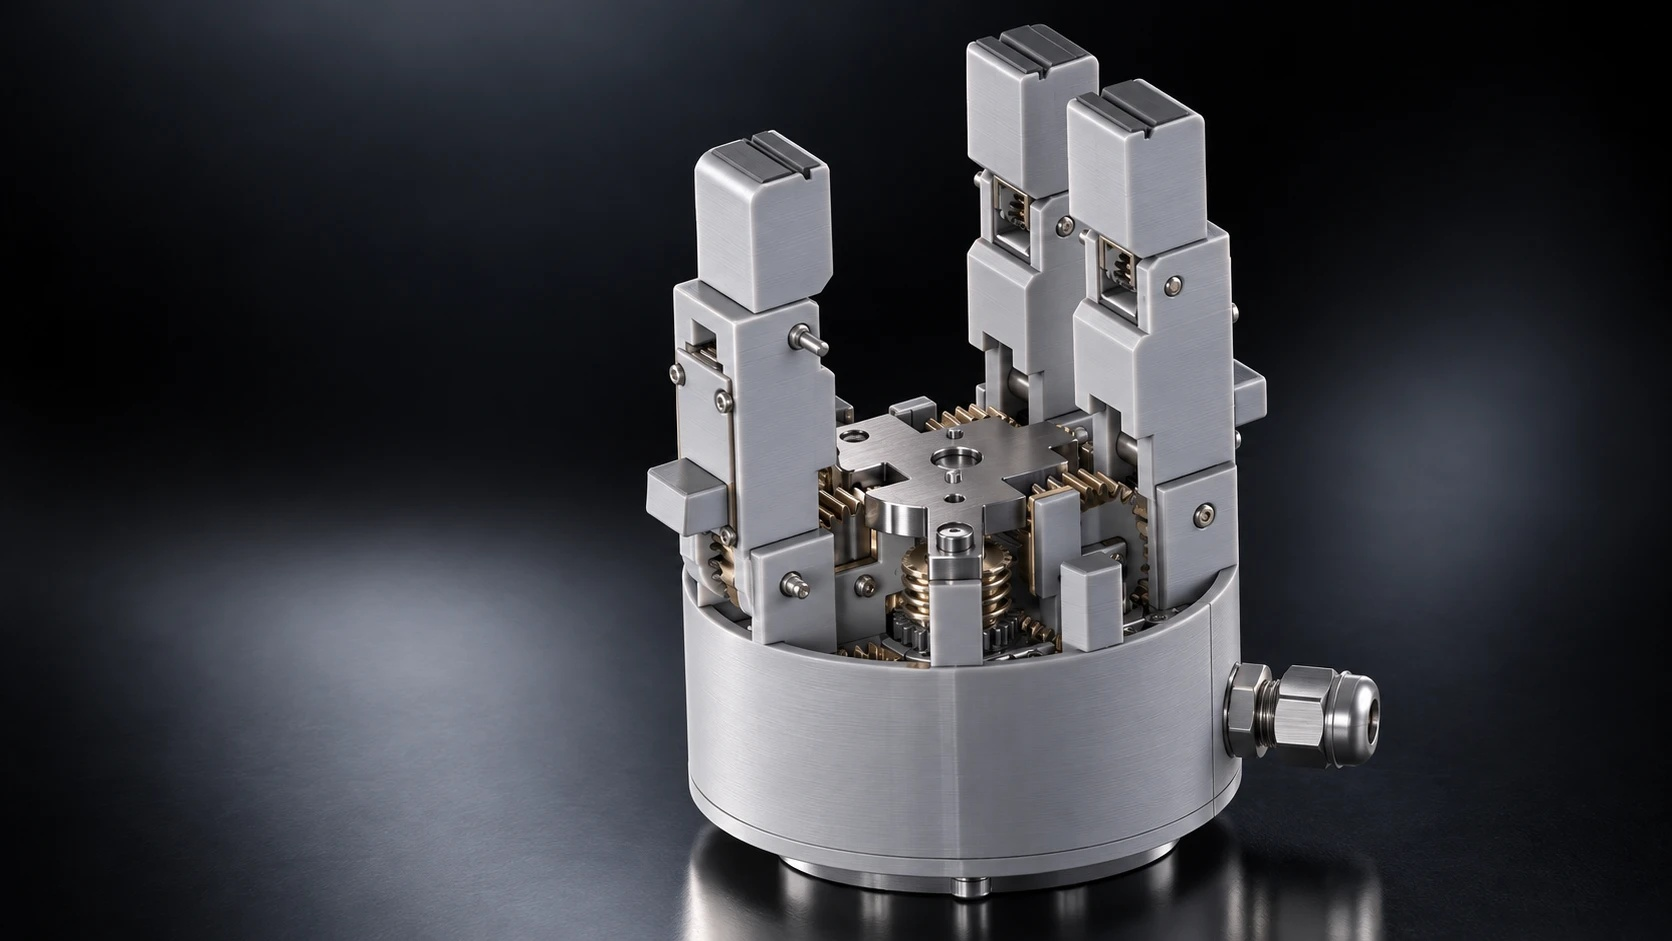
\includegraphics[width=0.85\textwidth]{gripper_hero_cad.jpg}\par
\vspace{2cm}
{\large Entrega Final\par}
\vspace{0.3cm}
{\large Octubre de 2026\par}
\end{titlepage}

\tableofcontents
\newpage

% ======================================================================
\section{Introducción}
El presente informe desarrolla el diseño de detalle de un gripper robótico antropomórfico de tres dedos para el robot colaborativo UR5e, a partir del plano de medidas GV24-MED-01 (versión V2.4) y del ensamble CAD del mecanismo. Cada dedo tiene dos falanges, proximal (L1) y distal (L2), articuladas en las juntas MCP y PIP.

La arquitectura emplea cuatro motores. Un motor central (servo) mueve un sinfín de módulo 1 que acciona, mediante un par de engranes z20, las tres ruedas z30 que a su vez mueven el piñón z12 de cada articulación MCP. Además, cada dedo tiene un motor N20 propio alojado en la falange proximal, que acciona la articulación PIP mediante un sinfín de módulo 0.5 y una rueda z16.

En el documento se desarrollan los cálculos estáticos en las vistas lateral, superior y frontal (punto 3.1), los cálculos cinemáticos de posición, velocidad y aceleración lineal y angular (punto 3.3) y los cálculos dinámicos con las estimaciones de potencia y consumo energético (punto 3.4). Los resultados analíticos se validan con dos modelos construidos en Working Model 2D.

% ======================================================================
\section{Objetivos}
\subsection{Objetivo general}
Determinar las fuerzas, torques, velocidades, aceleraciones y potencias del gripper de tres dedos V2.4 en sus configuraciones de agarre, y validar los resultados mediante simulación en Working Model 2D.

\subsection{Objetivos específicos}
\begin{itemize}
\item Identificar las transmisiones del mecanismo y su relación con los cuatro motores.
\item Calcular las fuerzas, torques y reacciones del sistema en las vistas lateral, superior y frontal para agarres tipo pinch y power.
\item Determinar los torques requeridos en las articulaciones MCP y PIP de cada dedo solo con las medidas del mecanismo, sin considerar la transmisión de engranajes.
\item Describir los desplazamientos, velocidades y aceleraciones lineales y angulares de las falanges durante el cierre.
\item Estimar la potencia y la energía consumidas en un ciclo de cierre y durante la retención del objeto.
\item Comparar el cálculo analítico con los resultados de Working Model 2D y reportar el error porcentual.
\end{itemize}

% ======================================================================
\section{Datos de entrada}
\subsection{Plano de medidas V2.4}
Los cálculos usan exclusivamente la geometría, las masas y las transmisiones del plano GV24-MED-01 (Figura \ref{fig:plano}). Los parámetros que el plano no define se tratan como variables y se identifican como \emph{dato faltante}.

\begin{figure}[H]
\centering
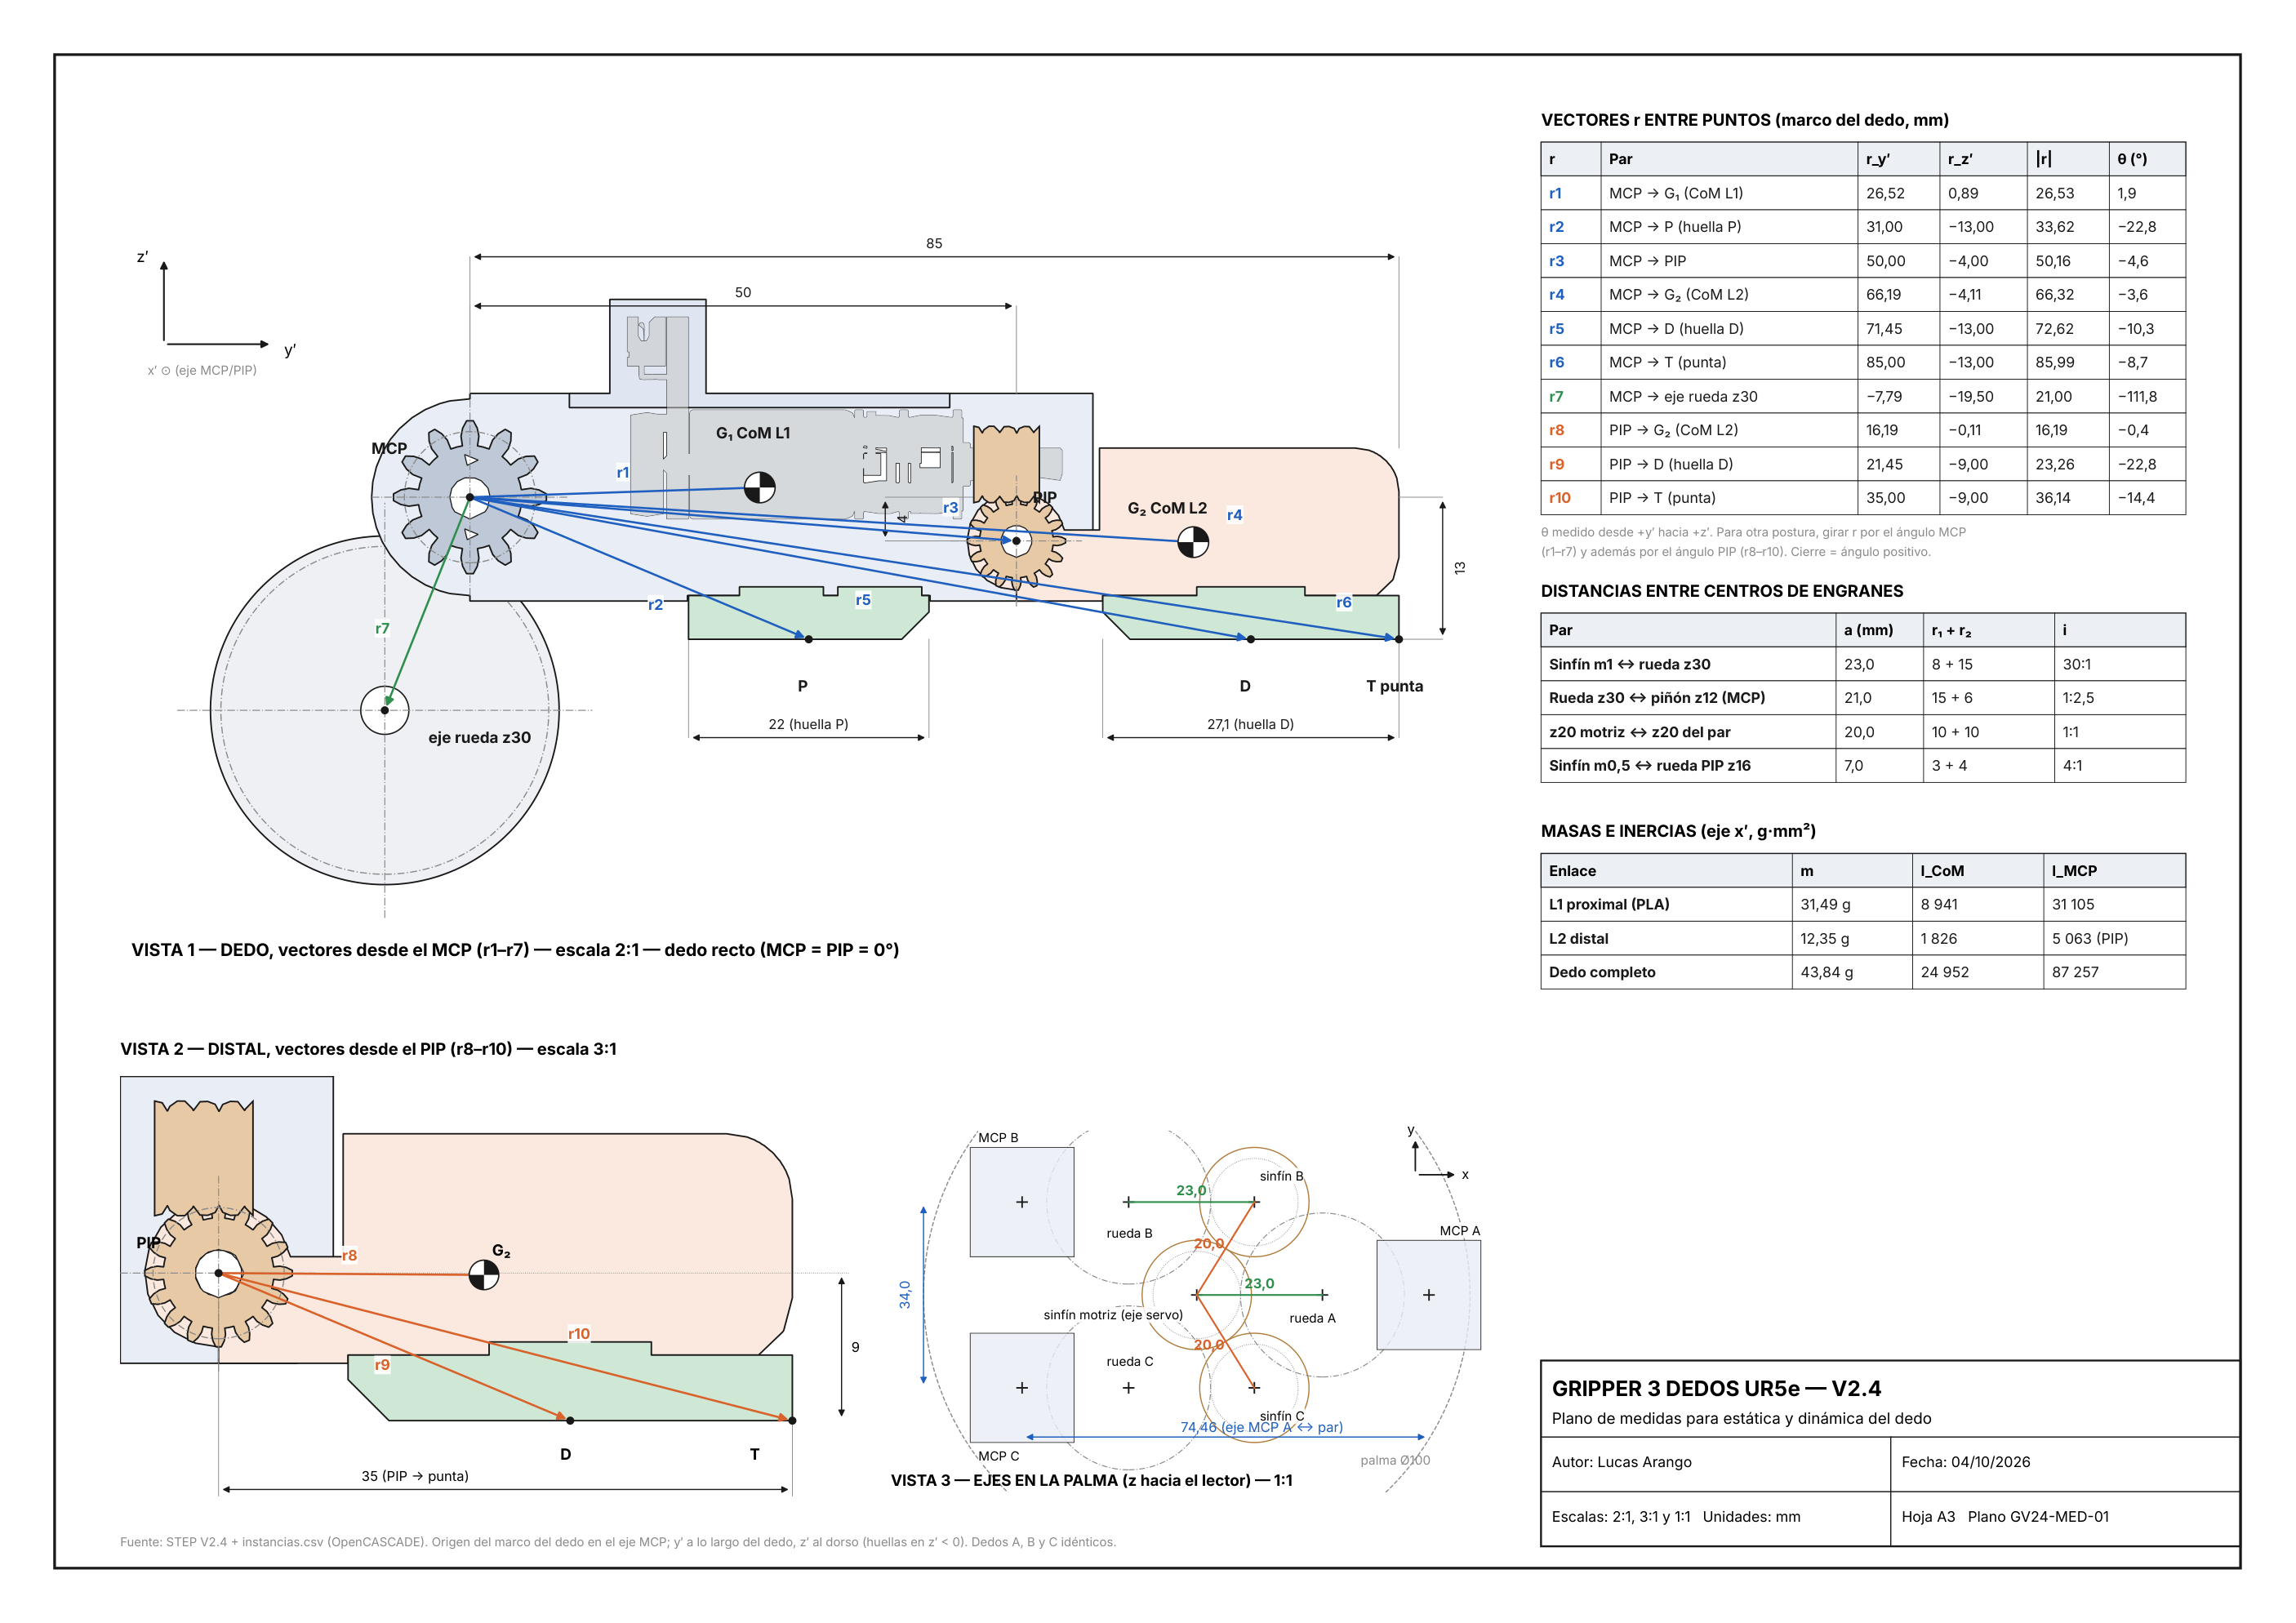
\includegraphics[width=\textwidth]{plano_v24.png}
\caption{Plano de medidas GV24-MED-01 del dedo y de la palma.}
\label{fig:plano}
\end{figure}

\begin{table}[H]
\centering
\begin{tabular}{|c|l|r|r|}
\hline
\textbf{Vector} & \textbf{Par} & \textbf{$r_{y'}$ [mm]} & \textbf{$r_{z'}$ [mm]} \\ \hline
r1 & MCP $\rightarrow$ G$_1$ (CoM L1) & 26.52 & 0.89 \\ \hline
r2 & MCP $\rightarrow$ P (huella P) & 31.00 & $-13.00$ \\ \hline
r3 & MCP $\rightarrow$ PIP & 50.00 & $-4.00$ \\ \hline
r4 & MCP $\rightarrow$ G$_2$ (CoM L2) & 66.19 & $-4.11$ \\ \hline
r5 & MCP $\rightarrow$ D (huella D) & 71.45 & $-13.00$ \\ \hline
r6 & MCP $\rightarrow$ T (punta) & 85.00 & $-13.00$ \\ \hline
r7 & MCP $\rightarrow$ eje rueda z30 & $-7.79$ & $-19.50$ \\ \hline
r8 & PIP $\rightarrow$ G$_2$ & 16.19 & $-0.11$ \\ \hline
r9 & PIP $\rightarrow$ D & 21.45 & $-9.00$ \\ \hline
r10 & PIP $\rightarrow$ T & 35.00 & $-9.00$ \\ \hline
\end{tabular}
\caption{Vectores de posición del plano V2.4 (dedo recto).}
\label{tab:vectores}
\end{table}

\begin{table}[H]
\centering
\begin{tabular}{|l|r|r|r|}
\hline
\textbf{Eslabón} & \textbf{Masa [g]} & \textbf{$I_{CoM}$ [g$\cdot$mm$^2$]} & \textbf{$I_{eje}$ [g$\cdot$mm$^2$]} \\ \hline
L1 proximal & 31.49 & 8\,941 & 31\,105 (MCP) \\ \hline
L2 distal & 12.35 & 1\,826 & 5\,063 (PIP) \\ \hline
Dedo completo & 43.84 & 24\,952 & 87\,257 (MCP) \\ \hline
\end{tabular}
\caption{Masas e inercias del plano V2.4.}
\label{tab:masas}
\end{table}

\subsection{Transmisiones y motores}
\begin{table}[H]
\centering
\begin{tabular}{|l|r|r|l|}
\hline
\textbf{Tren} & \textbf{$a$ [mm]} & \textbf{$i$} & \textbf{Motor y función} \\ \hline
Sinfín m1 $\leftrightarrow$ rueda z30 & 23.0 & 30:1 & Central $\rightarrow$ rueda z30 de cada dedo \\ \hline
z20 motriz $\leftrightarrow$ z20 & 20.0 & 1:1 & Central $\rightarrow$ sinfines B y C \\ \hline
Rueda z30 $\leftrightarrow$ piñón z12 & 21.0 & 1:2.5 & MCP de cada dedo \\ \hline
Sinfín m0.5 $\leftrightarrow$ rueda z16 & 7.0 & 4:1 & N20 de cada dedo $\rightarrow$ PIP \\ \hline
\end{tabular}
\caption{Transmisiones del plano y su asignación a los motores.}
\label{tab:trenes}
\end{table}

La relación total entre el motor central y cada MCP es $i_{MCP} = 30 \times \frac{12}{30} = 12$, igual en las tres ramas, por lo que en el modo central se cumple $\theta_{MCP,A} = \theta_{MCP,B} = \theta_{MCP,C}$. La relación entre cada motor N20 y su PIP es $i_{PIP} = 4$.

% ======================================================================
\section{Cálculos estáticos (3.1)}
\subsection{Descripción}
El análisis estático determina las fuerzas, torques y momentos en el gripper durante la sujeción de un objeto cilíndrico. Se estudian tres vistas: la vista lateral, que contiene el plano de flexión de cada dedo y las articulaciones MCP y PIP; la vista superior, que corresponde al plano de la palma y muestra el equilibrio entre los tres dedos y las fuerzas en los engranes; y la vista frontal, que contiene el eje del gripper y permite obtener la reacción transmitida a la brida del UR5e.

\subsection{Objetivo de cálculo}
\begin{itemize}
\item Determinar las posiciones de los puntos de contacto P, D y T y de los centros de masa para cada postura.
\item Calcular los torques requeridos en las articulaciones MCP y PIP y las reacciones en ambas juntas.
\item Calcular la fuerza normal mínima para sujetar objetos de 1 a 4 kg con $\mu$ de 0.3, 0.5 y 0.7.
\item Obtener los torques en las articulaciones MCP y PIP de cada dedo y el caso crítico de todo el barrido, sin considerar la transmisión de engranajes.
\end{itemize}

\subsection{Variables del modelo de cálculo}
\begin{table}[H]
\centering
\begin{tabular}{|l|l|}
\hline
\textbf{Variable} & \textbf{Descripción} \\ \hline
$\theta_{MCP}$, $\theta_{PIP}$ & Ángulos articulares de cierre (0°, 15°, 30°, 45°, 60° y 0°, 15°, 30°, 45°) \\ \hline
$m$, $W$ & Masa y peso del objeto (1 a 4 kg) \\ \hline
$\mu$ & Coeficiente de fricción en el contacto (0.3, 0.5, 0.7) \\ \hline
$N$, $F_t$ & Fuerza normal y tangencial de contacto por dedo \\ \hline
$\tau_{MCP}$, $\tau_{PIP}$ & Torques requeridos en las articulaciones \\ \hline
$R_{MCP}$, $R_{PIP}$ & Reacciones en las juntas \\ \hline
\end{tabular}
\caption{Variables del modelo estático.}
\label{tab:varest}
\end{table}

\subsection{Modelo de cálculo}
Se usa un marco fijo a la palma con origen en el eje MCP, con $y'$ a lo largo del dedo recto y $z'$ hacia el dorso. El ángulo de cierre es positivo de $+y'$ hacia $-z'$. Los vectores r1 a r7 se rotan con $\theta_{MCP}$ y r8 a r10 con $\theta_{MCP}+\theta_{PIP}$:
\eq{y = r_y\cos\theta + r_z\sin\theta \qquad z = -r_y\sin\theta + r_z\cos\theta}

El torque requerido en una articulación, positivo en el sentido de cierre, se obtiene con las coordenadas reales del punto de aplicación de cada fuerza:
\eq{\tau = \sum_i \left( y_i F_{z,i} - z_i F_{y,i} \right)}

Con los actuadores tratados como pares puros, las reacciones son:
\eq{R_{PIP} = -\left(F_{L2} + m_2 g\right) \qquad R_{MCP} = -\left(F_{c} + m_1 g + m_2 g\right)}

La condición de no deslizamiento define la fuerza normal mínima por dedo:
\eq{2\mu N \geq W \;\;(\text{pinch}) \qquad 3\mu N \geq W \;\;(\text{power})}

El análisis estático no considera el mecanismo ni la transmisión de engranajes: los resultados son las fuerzas y los torques en los puntos de interés del dedo (contactos P, D y T y articulaciones MCP y PIP), obtenidos solo con las medidas del plano.

\subsection{Valores del modelo de cálculo}
Se evalúan 5 ángulos MCP $\times$ 4 ángulos PIP, contactos en P, D y T, masas de 1, 2, 3 y 4 kg y $\mu$ de 0.3, 0.5 y 0.7. Se considera $g = 9.81$ m/s$^2$ con el gripper orientado hacia abajo, que es la condición de recogida del UR5e.

\begin{table}[H]
\centering
\small
\begin{adjustbox}{max width=\textwidth}
\begin{tabular}{|c|c|c|c|c|c|}
\hline
\textbf{$\theta_{MCP}/\theta_{PIP}$} & \textbf{P} & \textbf{D} & \textbf{T} & \textbf{G$_1$} & \textbf{G$_2$} \\ \hline
0° / 0° & (31.0, -13.0) & (71.5, -13.0) & (85.0, -13.0) & (26.5, 0.9) & (66.2, -4.1) \\ \hline
0° / 15° & (31.0, -13.0) & (68.4, -18.2) & (81.5, -21.8) & (26.5, 0.9) & (65.6, -8.3) \\ \hline
0° / 30° & (31.0, -13.0) & (64.1, -22.5) & (75.8, -29.3) & (26.5, 0.9) & (64.0, -12.2) \\ \hline
0° / 45° & (31.0, -13.0) & (58.8, -25.5) & (68.4, -35.1) & (26.5, 0.9) & (61.4, -15.5) \\ \hline
15° / 0° & (26.6, -20.6) & (65.7, -31.0) & (78.7, -34.6) & (25.8, -6.0) & (62.9, -21.1) \\ \hline
15° / 15° & (26.6, -20.6) & (61.3, -35.3) & (73.1, -42.1) & (25.8, -6.0) & (61.2, -25.0) \\ \hline
15° / 30° & (26.6, -20.6) & (56.1, -38.3) & (65.6, -47.9) & (25.8, -6.0) & (58.6, -28.3) \\ \hline
15° / 45° & (26.6, -20.6) & (50.2, -39.9) & (57.0, -51.6) & (25.8, -6.0) & (55.3, -30.9) \\ \hline
30° / 0° & (20.3, -26.8) & (55.4, -47.0) & (67.1, -53.8) & (23.4, -12.5) & (55.3, -36.7) \\ \hline
30° / 15° & (20.3, -26.8) & (50.1, -50.0) & (59.7, -59.6) & (23.4, -12.5) & (52.7, -40.0) \\ \hline
30° / 30° & (20.3, -26.8) & (44.2, -51.5) & (51.0, -63.3) & (23.4, -12.5) & (49.3, -42.5) \\ \hline
30° / 45° & (20.3, -26.8) & (38.2, -51.5) & (41.7, -64.6) & (23.4, -12.5) & (45.4, -44.1) \\ \hline
45° / 0° & (12.7, -31.1) & (41.3, -59.7) & (50.9, -69.3) & (19.4, -18.1) & (43.9, -49.7) \\ \hline
45° / 15° & (12.7, -31.1) & (35.5, -61.3) & (42.2, -73.0) & (19.4, -18.1) & (40.5, -52.3) \\ \hline
45° / 30° & (12.7, -31.1) & (29.4, -61.2) & (32.9, -74.3) & (19.4, -18.1) & (36.6, -53.9) \\ \hline
45° / 45° & (12.7, -31.1) & (23.5, -59.6) & (23.5, -73.2) & (19.4, -18.1) & (32.4, -54.4) \\ \hline
60° / 0° & (4.2, -33.3) & (24.5, -68.4) & (31.2, -80.1) & (14.0, -22.5) & (29.5, -59.4) \\ \hline
60° / 15° & (4.2, -33.3) & (18.4, -68.3) & (21.9, -81.4) & (14.0, -22.5) & (25.6, -61.0) \\ \hline
60° / 30° & (4.2, -33.3) & (12.5, -66.8) & (12.5, -80.3) & (14.0, -22.5) & (21.4, -61.5) \\ \hline
60° / 45° & (4.2, -33.3) & (7.3, -63.7) & (3.8, -76.8) & (14.0, -22.5) & (17.2, -60.9) \\ \hline
\end{tabular}
\end{adjustbox}
\caption{Posiciones $(y', z')$ en mm de los puntos característicos para las 20 posturas.}
\label{tab:posiciones}
\end{table}
\begin{table}[H]
\centering
\small
\begin{adjustbox}{max width=\textwidth}
\begin{tabular}{|c|r|r|r|r|r|r|}
\hline
\textbf{$\theta_{MCP}/\theta_{PIP}$} & \textbf{$\tau_{g,MCP}$} & \textbf{$\tau_{g,PIP}$} & \textbf{$\tau_{g,MCP}^{peor}$} & \textbf{$\tau_{g,PIP}^{peor}$} & \textbf{$R_{MCP}$} & \textbf{$R_{PIP}$} \\ \hline
0° / 0° & 0.22 & 0.01 & 16.21 & 1.96 & 0.430 & 0.121 \\ \hline
0° / 15° & 0.73 & 0.52 & 16.16 & 1.96 & 0.430 & 0.121 \\ \hline
0° / 30° & 1.20 & 0.99 & 15.99 & 1.96 & 0.430 & 0.121 \\ \hline
0° / 45° & 1.61 & 1.40 & 15.71 & 1.96 & 0.430 & 0.121 \\ \hline
15° / 0° & 4.41 & 0.52 & 16.21 & 1.96 & 0.430 & 0.121 \\ \hline
15° / 15° & 4.88 & 0.99 & 16.16 & 1.96 & 0.430 & 0.121 \\ \hline
15° / 30° & 5.29 & 1.40 & 15.99 & 1.96 & 0.430 & 0.121 \\ \hline
15° / 45° & 5.60 & 1.71 & 15.71 & 1.96 & 0.430 & 0.121 \\ \hline
30° / 0° & 8.30 & 0.99 & 16.21 & 1.96 & 0.430 & 0.121 \\ \hline
30° / 15° & 8.70 & 1.40 & 16.16 & 1.96 & 0.430 & 0.121 \\ \hline
30° / 30° & 9.01 & 1.71 & 15.99 & 1.96 & 0.430 & 0.121 \\ \hline
30° / 45° & 9.20 & 1.90 & 15.71 & 1.96 & 0.430 & 0.121 \\ \hline
45° / 0° & 11.62 & 1.40 & 16.21 & 1.96 & 0.430 & 0.121 \\ \hline
45° / 15° & 11.93 & 1.71 & 16.16 & 1.96 & 0.430 & 0.121 \\ \hline
45° / 30° & 12.12 & 1.90 & 15.99 & 1.96 & 0.430 & 0.121 \\ \hline
45° / 45° & 12.19 & 1.96 & 15.71 & 1.96 & 0.430 & 0.121 \\ \hline
60° / 0° & 14.15 & 1.71 & 16.21 & 1.96 & 0.430 & 0.121 \\ \hline
60° / 15° & 14.34 & 1.90 & 16.16 & 1.96 & 0.430 & 0.121 \\ \hline
60° / 30° & 14.41 & 1.96 & 15.99 & 1.96 & 0.430 & 0.121 \\ \hline
60° / 45° & 14.34 & 1.89 & 15.71 & 1.96 & 0.430 & 0.121 \\ \hline
\end{tabular}
\end{adjustbox}
\caption{Torques gravitacionales (mN$\cdot$m) y reacciones (N) del dedo sin carga, gripper hacia abajo.}
\label{tab:gravedad}
\end{table}

\subsection{Resultados vista lateral}
La Figura \ref{fig:lateral} muestra el diagrama de cuerpo libre del dedo A en un pinch de 4 kg con contacto en la punta. La normal de contacto genera el torque dominante: los efectos gravitacionales del propio dedo son menores al 0.5 \% del torque de agarre (Tabla \ref{tab:gravedad}).

\begin{figure}[H]
\centering
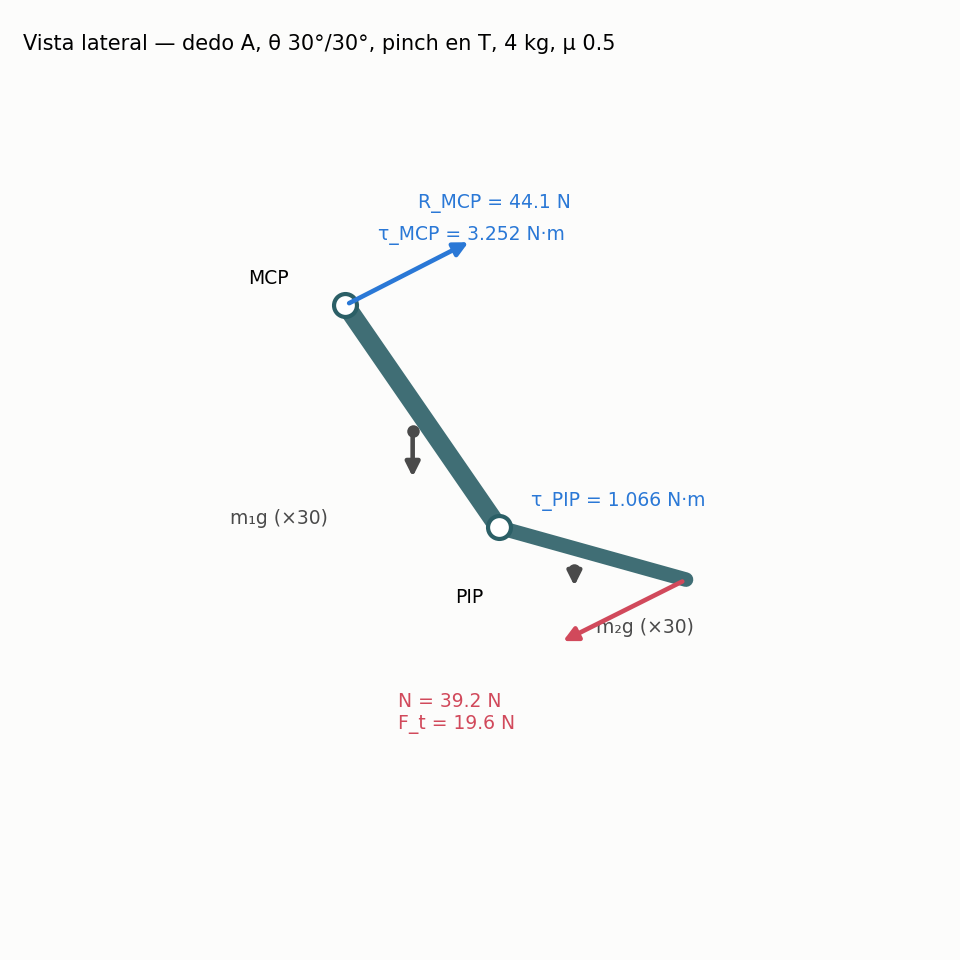
\includegraphics[width=0.62\textwidth]{D6_vista_lateral_DCL.png}
\caption{Diagrama de cuerpo libre en vista lateral del dedo A.}
\label{fig:lateral}
\end{figure}
\par\noindent\textbf{Análisis.} En un pinch de 4 kg en la punta, el torque en el MCP (3.252 N$\cdot$m) es unas tres veces el del PIP (1.066 N$\cdot$m), porque la normal en T actúa con un brazo mucho mayor respecto al MCP. El peso propio del dedo aporta menos del 0.5 \% del torque, así que el dimensionamiento lo fija la fuerza de agarre.




\begin{table}[H]
\centering

\begin{adjustbox}{max width=\textwidth}
\begin{tabular}{|c|r|r|r|r|r|r|r|}
\hline
\textbf{Masa [kg]} & \textbf{W [N]} & \textbf{Pinch 0.3} & \textbf{Pinch 0.5} & \textbf{Pinch 0.7} & \textbf{Power 0.3} & \textbf{Power 0.5} & \textbf{Power 0.7} \\ \hline
1 & 9.81 & 16.35 & 9.81 & 7.01 & 10.90 & 6.54 & 4.67 \\ \hline
2 & 19.62 & 32.70 & 19.62 & 14.01 & 21.80 & 13.08 & 9.34 \\ \hline
3 & 29.43 & 49.05 & 29.43 & 21.02 & 32.70 & 19.62 & 14.01 \\ \hline
4 & 39.24 & 65.40 & 39.24 & 28.03 & 43.60 & 26.16 & 18.69 \\ \hline
\end{tabular}
\end{adjustbox}
\caption{Fuerza normal mínima por dedo [N]: pinch $2\mu N \geq W$ y power $3\mu N \geq W$.}
\label{tab:nmin}
\end{table}
\begin{table}[H]
\centering
\small
\begin{adjustbox}{max width=\textwidth}
\begin{tabular}{|c|c|r|r|r|r|r|r|r|r|r|}
\hline
\textbf{Cont.} & \textbf{$\mu$} & \textbf{$N$ [N]} & \textbf{$\tau_{MCP}$} & \textbf{$\tau_{PIP}$} & \textbf{$R_{MCP}$} & \textbf{$R_{PIP}$} & \textbf{$T_c^{\eta=0.5}$} & \textbf{$T_c^{\eta=0.8}$} & \textbf{$T_A^{\eta=0.5}$} & \textbf{$T_A^{\eta=0.8}$} \\ \hline
P & 0.30 & 65.40 & 1.865 & 0.002 & 68.40 & 0.12 & 0.623 & 0.389 & 0.001 & 0.001 \\ \hline
P & 0.50 & 39.24 & 1.332 & 0.002 & 44.07 & 0.12 & 0.446 & 0.279 & 0.001 & 0.001 \\ \hline
P & 0.70 & 28.03 & 1.104 & 0.002 & 34.46 & 0.12 & 0.370 & 0.231 & 0.001 & 0.001 \\ \hline
D & 0.30 & 65.40 & 3.913 & 0.646 & 68.40 & 68.31 & 1.306 & 0.816 & 0.323 & 0.202 \\ \hline
D & 0.50 & 39.24 & 2.756 & 0.569 & 44.07 & 43.93 & 0.920 & 0.575 & 0.285 & 0.178 \\ \hline
D & 0.70 & 28.03 & 2.260 & 0.537 & 34.46 & 34.28 & 0.755 & 0.472 & 0.268 & 0.168 \\ \hline
T & 0.30 & 65.40 & 4.586 & 1.319 & 68.40 & 68.31 & 1.530 & 0.956 & 0.660 & 0.412 \\ \hline
T & 0.50 & 39.24 & 3.252 & 1.066 & 44.07 & 43.93 & 1.085 & 0.678 & 0.533 & 0.333 \\ \hline
T & 0.70 & 28.03 & 2.680 & 0.957 & 34.46 & 34.28 & 0.895 & 0.559 & 0.478 & 0.299 \\ \hline
\end{tabular}
\end{adjustbox}
\caption{Pinch de 4 kg con dedos A y B, $\theta = 30°/30°$. Torques en N$\cdot$m, fuerzas en N.}
\label{tab:pinch}
\end{table}
\begin{table}[H]
\centering
\small
\begin{adjustbox}{max width=\textwidth}
\begin{tabular}{|c|c|r|r|r|r|r|r|r|r|}
\hline
\textbf{Disp.} & \textbf{Cont.} & \textbf{$N_A$} & \textbf{$N_B$} & \textbf{$\tau_{MCP,A}$} & \textbf{$\tau_{MCP,B}$} & \textbf{$\tau_{PIP,A}$} & \textbf{$\tau_{PIP,B}$} & \textbf{$R_{MCP,A}$} & \textbf{$R_{PIP,A}$} \\ \hline
120° & P & 26.16 & 26.16 & 0.891 & 0.891 & 0.002 & 0.002 & 29.44 & 0.12 \\ \hline
Plano & P & 39.24 & 19.62 & 1.332 & 0.671 & 0.002 & 0.002 & 44.07 & 0.12 \\ \hline
120° & D & 26.16 & 26.16 & 1.840 & 1.840 & 0.380 & 0.380 & 29.44 & 29.30 \\ \hline
Plano & D & 39.24 & 19.62 & 2.756 & 1.382 & 0.569 & 0.286 & 44.07 & 43.93 \\ \hline
120° & T & 26.16 & 26.16 & 2.171 & 2.171 & 0.711 & 0.711 & 29.44 & 29.30 \\ \hline
Plano & T & 39.24 & 19.62 & 3.252 & 1.630 & 1.066 & 0.534 & 44.07 & 43.93 \\ \hline
120° & PD & 26.16 & 26.16 & 1.366 & 1.366 & 0.191 & 0.191 & 29.44 & 14.68 \\ \hline
Plano & PD & 39.24 & 19.62 & 2.044 & 1.027 & 0.286 & 0.144 & 44.07 & 21.99 \\ \hline
\end{tabular}
\end{adjustbox}
\caption{Power grasp de 4 kg, $\mu=0.5$, $\theta = 30°/30°$. Torques en las articulaciones en N$\cdot$m, fuerzas en N.}
\label{tab:power}
\end{table}
\begin{table}[H]
\centering
\small
\begin{adjustbox}{max width=\textwidth}
\begin{tabular}{|c|r|r|r|r|r|r|r|r|r|r|}
\hline
\textbf{Cont.} & \textbf{$N_A$} & \textbf{$N_B$} & \textbf{$N_C$} & \textbf{$\tau_{MCP,A}$} & \textbf{$\tau_{MCP,B}$} & \textbf{$\tau_{MCP,C}$} & \textbf{$T_c$} & \textbf{$T_A$} & \textbf{$T_B$} & \textbf{$T_C$} \\ \hline
P & 31.39 & 27.47 & 19.62 & 1.068 & 0.935 & 0.671 & 0.371 & 0.001 & 0.001 & 0.001 \\ \hline
D & 31.39 & 27.47 & 19.62 & 2.207 & 1.932 & 1.382 & 0.767 & 0.190 & 0.166 & 0.119 \\ \hline
T & 31.39 & 27.47 & 19.62 & 2.603 & 2.279 & 1.630 & 0.905 & 0.355 & 0.311 & 0.222 \\ \hline
PD & 31.39 & 27.47 & 19.62 & 1.637 & 1.434 & 1.027 & 0.569 & 0.095 & 0.084 & 0.060 \\ \hline
\end{tabular}
\end{adjustbox}
\caption{Carga desigual A 40 \%, B 35 \%, C 25 \% (4 kg, $\mu=0.5$, $\theta=30°/30°$, $\eta=0.6$).}
\label{tab:desigual}
\end{table}

\subsection{Resultados vista superior}
En el plano de la palma los tres dedos aplican sus fuerzas normales sobre el objeto. Según el plano V2.4, el dedo A se opone a los dedos B y C, que son paralelos y están separados 34 mm, por lo que el equilibrio horizontal exige $N_A = N_B + N_C$. Esta condición hace que el dedo A soporte el doble de carga que B o C (Figura \ref{fig:superior}). Las fuerzas de B y C generan momentos de $\pm 0.334$ N$\cdot$m alrededor del eje del objeto que se anulan entre sí.

\begin{figure}[H]
\centering
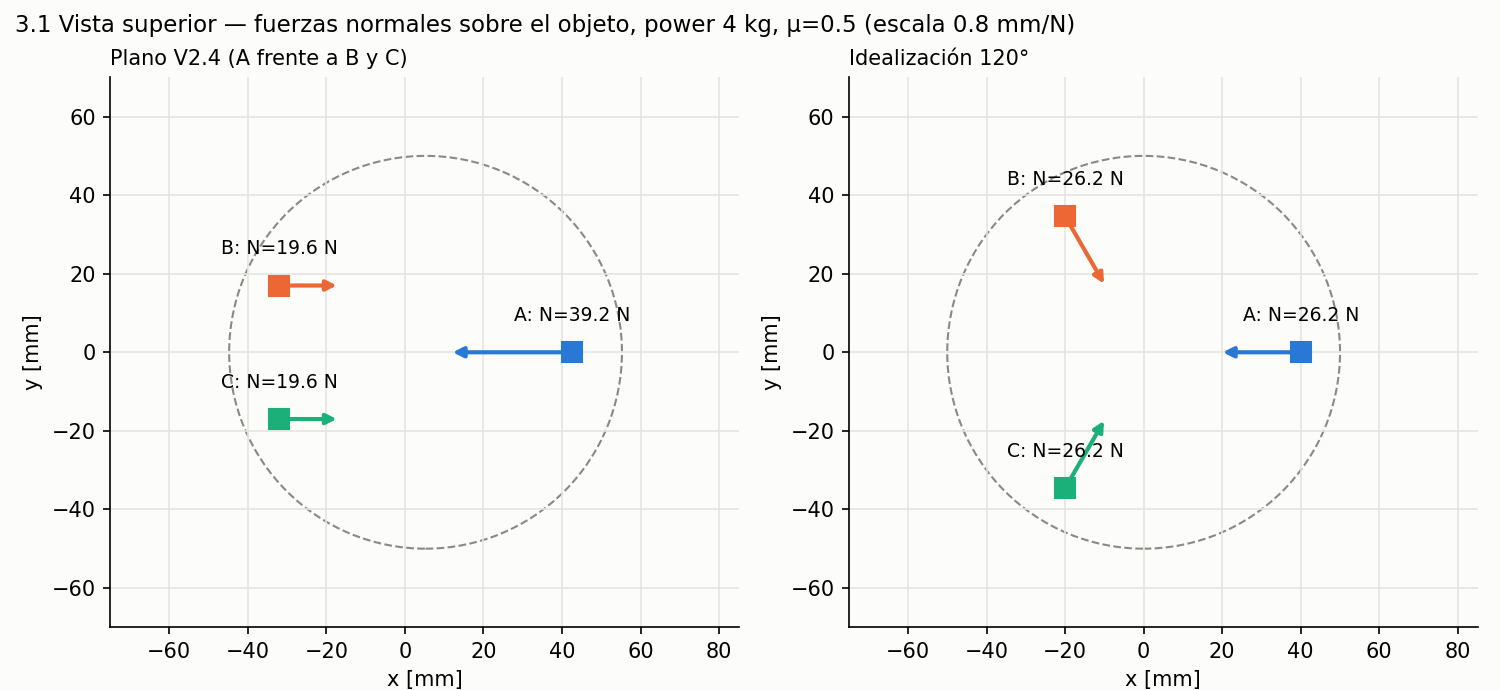
\includegraphics[width=\textwidth]{D5_vista_superior.png}
\caption{Fuerzas normales en vista superior según el plano y con la idealización a 120°.}
\label{fig:superior}
\end{figure}
\par\noindent\textbf{Análisis.} Con la disposición real del plano, el dedo A recibe 39.24 N, el doble que B y C (19.62 N cada uno); en la idealización a 120° los tres reciben 26.16 N. La suma de fuerzas es nula y los momentos de B y C ($\pm$0.334 N$\cdot$m) se cancelan, por lo que el objeto queda en equilibrio sin girar.




\begin{table}[H]
\centering

\begin{adjustbox}{max width=\textwidth}
\begin{tabular}{|c|r|r|r|r|r|r|}
\hline
\textbf{Dedo} & \textbf{$x$ [mm]} & \textbf{$y$ [mm]} & \textbf{$N$ [N]} & \textbf{$F_x$ [N]} & \textbf{$F_y$ [N]} & \textbf{$F_t$ [N]} \\ \hline
A & 42.49 & 0.00 & 39.24 & -39.24 & 0.00 & 19.62 \\ \hline
B & -31.96 & 17.00 & 19.62 & 19.62 & 0.00 & 9.81 \\ \hline
C & -31.96 & -17.00 & 19.62 & 19.62 & 0.00 & 9.81 \\ \hline
$\Sigma$ &  &  &  & 0.00 & 0.00 & 39.24 \\ \hline
\end{tabular}
\end{adjustbox}
\caption{Vista superior, power según plano, 4 kg, $\mu = 0.5$: fuerzas de los dedos sobre el objeto.}
\label{tab:superior}
\end{table}

\subsection{Resultados vista frontal}
En la vista frontal se obtiene la reacción en la brida del robot (Figura \ref{fig:frontal}). Con un objeto de 4 kg la brida soporta $F_z = 40.5$ N, que incluye el peso de los tres dedos, y un momento $M_y = 0.21$ N$\cdot$m debido a la excentricidad de 5.27 mm del eje del objeto. La masa de la palma, el servo y los motores N20 no está en el plano y se debe sumar a $F_z$.

\begin{figure}[H]
\centering
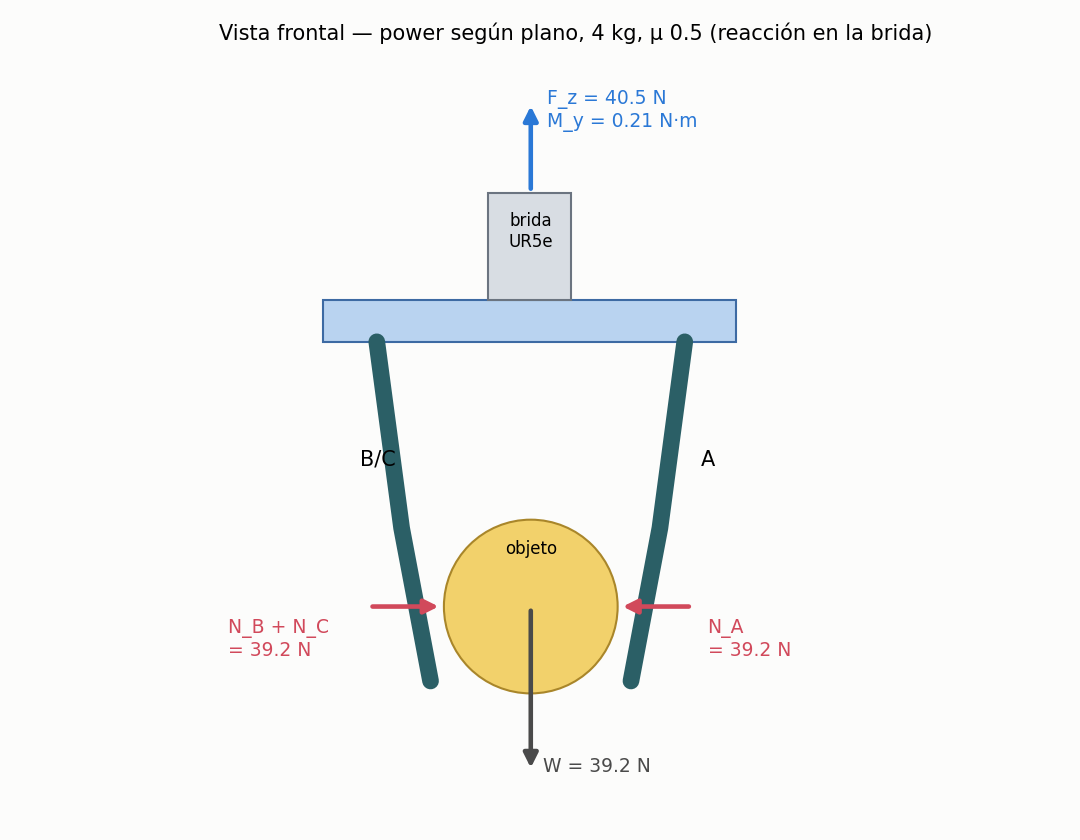
\includegraphics[width=0.62\textwidth]{D7_vista_frontal_DCL.png}
\caption{Diagrama de cuerpo libre en vista frontal del gripper con el objeto.}
\label{fig:frontal}
\end{figure}
\par\noindent\textbf{Análisis.} La brida soporta 40.5 N verticales: los 39.24 N del objeto más el peso de los dedos. El momento de 0.21 N$\cdot$m aparece porque el eje del objeto queda 5.27 mm desplazado del eje del gripper; es pequeño, pero crece con la masa, así que conviene centrar la pieza.




\subsection{Caso crítico}
\begin{table}[H]
\centering

\begin{adjustbox}{max width=\textwidth}
\begin{tabular}{|l|r|l|}
\hline
\textbf{Magnitud} & \textbf{Máximo} & \textbf{Configuración} \\ \hline
Torque MCP & 5.832 N$\cdot$m & pinch, T, 4 kg, $\mu$ 0.3, 15°/0° \\ \hline
Torque PIP & 2.466 N$\cdot$m & pinch, T, 4 kg, $\mu$ 0.3, 0°/0° \\ \hline
Fuerza de contacto $|F|$ & 68.280 N & pinch, P, 4 kg, $\mu$ 0.3, 0°/0° \\ \hline
Reacción MCP (par puro) & 68.404 N & pinch, P, 4 kg, $\mu$ 0.3, 0°/0° \\ \hline
Reacción PIP & 68.315 N & pinch, D, 4 kg, $\mu$ 0.3, 0°/0° \\ \hline
\end{tabular}
\end{adjustbox}
\caption{Caso crítico obtenido del barrido completo.}
\label{tab:critico}
\end{table}

% >>> graficas barrido
\subsection{Gráficas del barrido estático}
Las siguientes gráficas resumen el barrido estático completo. Debajo de cada una se comenta lo que muestran los datos.

\begin{figure}[H]
\centering
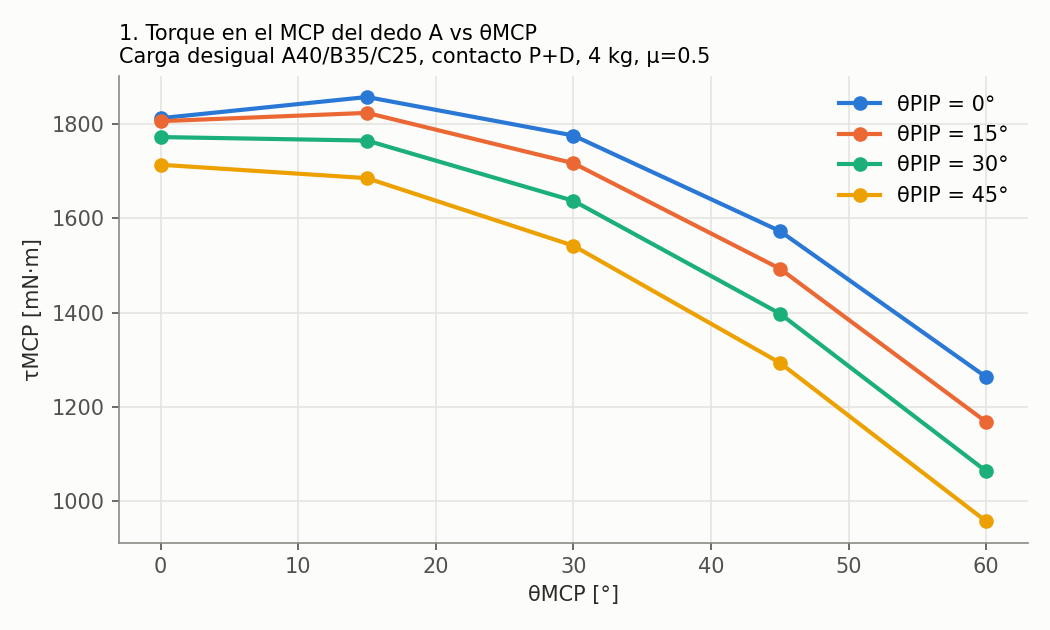
\includegraphics[width=0.8\textwidth]{01_tauMCP_A_vs_angulo.png}
\caption{Torque en el MCP del dedo A contra $\theta_{MCP}$ (carga desigual, contacto P+D, 4 kg, $\mu = 0.5$).}
\label{fig:g01}
\end{figure}
\par\noindent\textbf{Análisis.} El torque en el MCP del dedo A, que lleva el 40 \% de la carga, llega a 1.857 N$\cdot$m con el dedo casi recto ($\theta_{MCP}$ = 15°, $\theta_{PIP}$ = 0°) y baja a 0.957 N$\cdot$m en la postura 60°/45°. Al flexionar, los contactos se acercan al eje MCP y el brazo de la normal disminuye, así que el peor caso son los dedos casi rectos.


\begin{figure}[H]
\centering
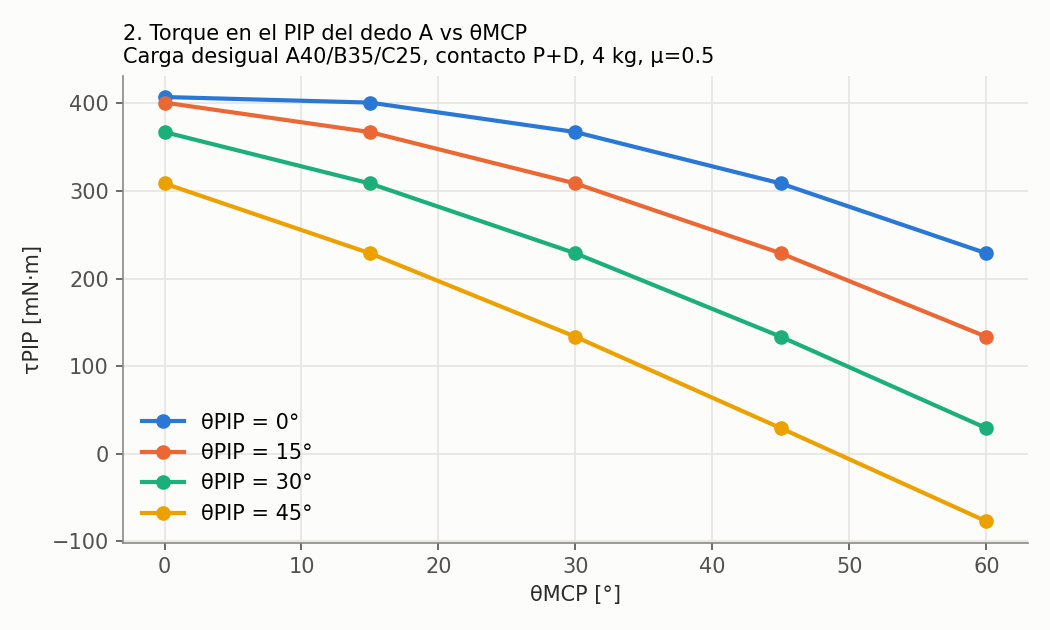
\includegraphics[width=0.8\textwidth]{02_tauPIP_A_vs_angulo.png}
\caption{Torque en el PIP del dedo A contra $\theta_{MCP}$.}
\label{fig:g02}
\end{figure}
\par\noindent\textbf{Análisis.} El torque en el PIP del dedo A llega a 0.407 N$\cdot$m con el dedo recto. Con $\theta_{MCP}$ = 60° y $\theta_{PIP}$ = 45° se vuelve negativo ($-$0.077 N$\cdot$m): la carga tiende a cerrar el PIP y la articulación debe frenar en lugar de empujar.


\begin{figure}[H]
\centering
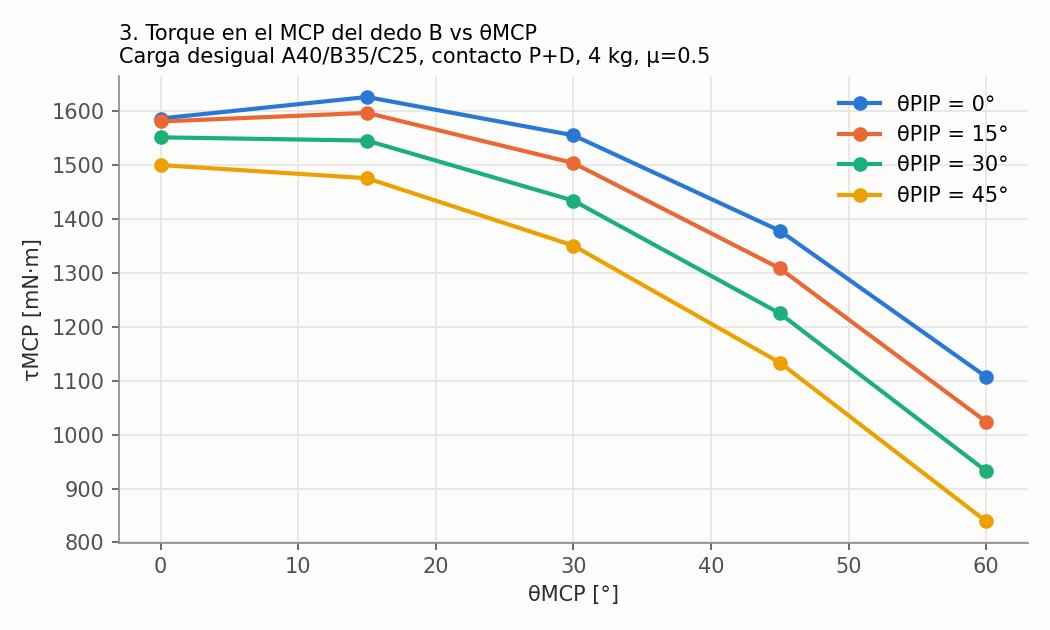
\includegraphics[width=0.8\textwidth]{03_tauMCP_B_vs_angulo.png}
\caption{Torque en el MCP del dedo B contra $\theta_{MCP}$.}
\label{fig:g03}
\end{figure}
\par\noindent\textbf{Análisis.} El dedo B sigue la misma tendencia que A con valores proporcionales a su 35 \% de la carga: de 1.626 N$\cdot$m con el dedo casi recto a 0.839 N$\cdot$m en la postura más cerrada.


\begin{figure}[H]
\centering
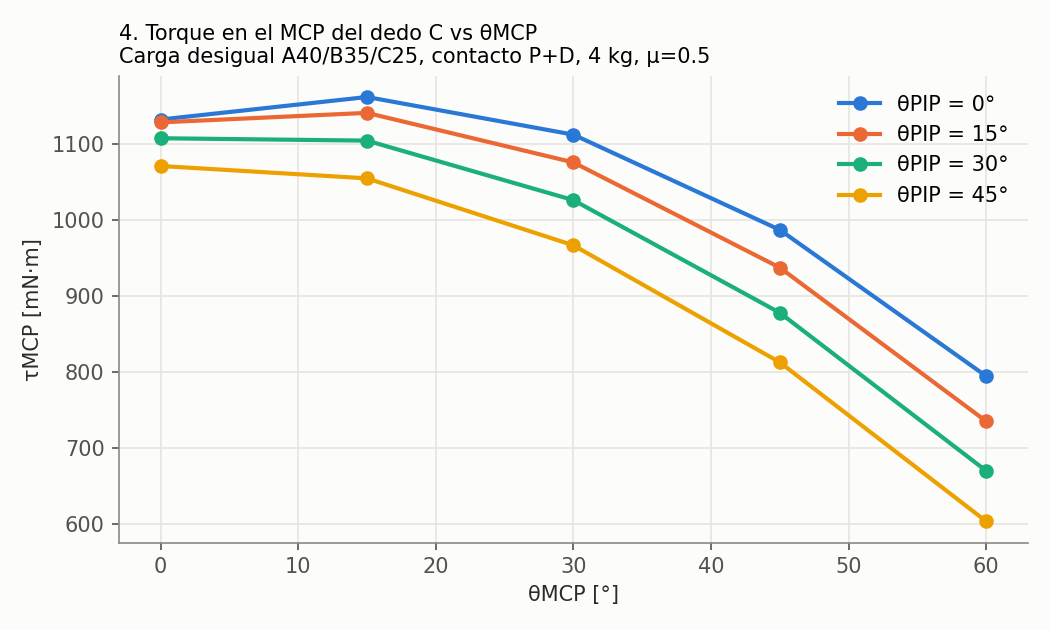
\includegraphics[width=0.8\textwidth]{04_tauMCP_C_vs_angulo.png}
\caption{Torque en el MCP del dedo C contra $\theta_{MCP}$.}
\label{fig:g04}
\end{figure}
\par\noindent\textbf{Análisis.} El dedo C, con el 25 \% de la carga, es el menos exigido (1.162 N$\cdot$m como máximo). Los torques de los tres dedos siguen exactamente la proporción del reparto, porque la geometría de los tres es la misma.


\begin{figure}[H]
\centering
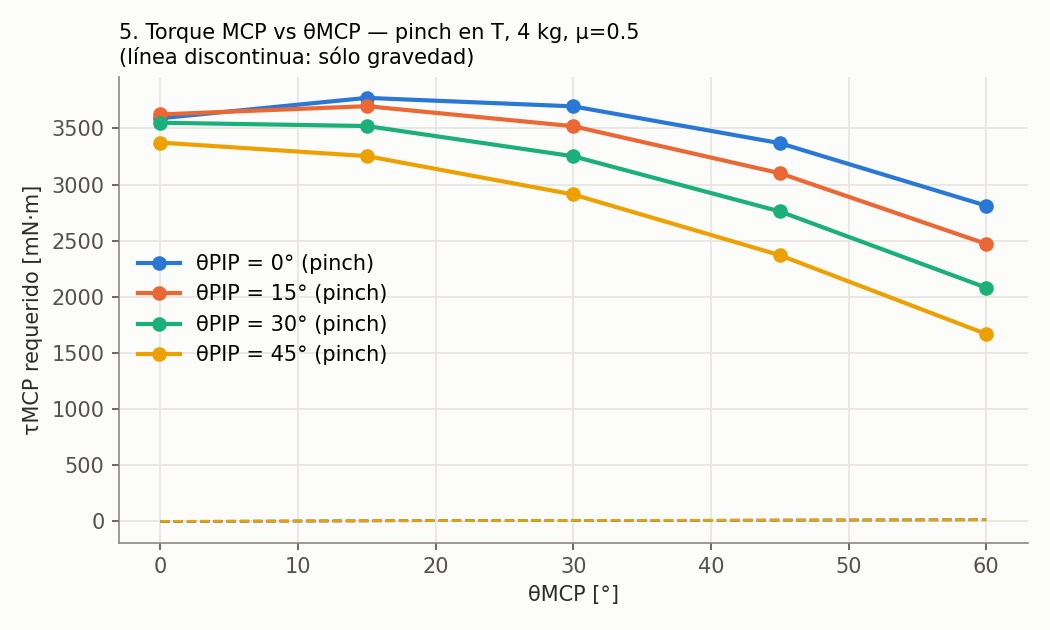
\includegraphics[width=0.8\textwidth]{05_tauMCP_vs_MCP.png}
\caption{Torque MCP requerido en pinch en la punta, 4 kg.}
\label{fig:g05}
\end{figure}
\par\noindent\textbf{Análisis.} En el pinch de 4 kg en la punta el torque MCP llega a 3.77 N$\cdot$m ($\theta_{MCP}$ = 15°, $\theta_{PIP}$ = 0°) y baja a 1.67 N$\cdot$m en la postura 60°/45°. La línea discontinua, que es solo la gravedad del dedo, queda por debajo de 15 mN$\cdot$m: menos del 0.5 \% del total.


\begin{figure}[H]
\centering
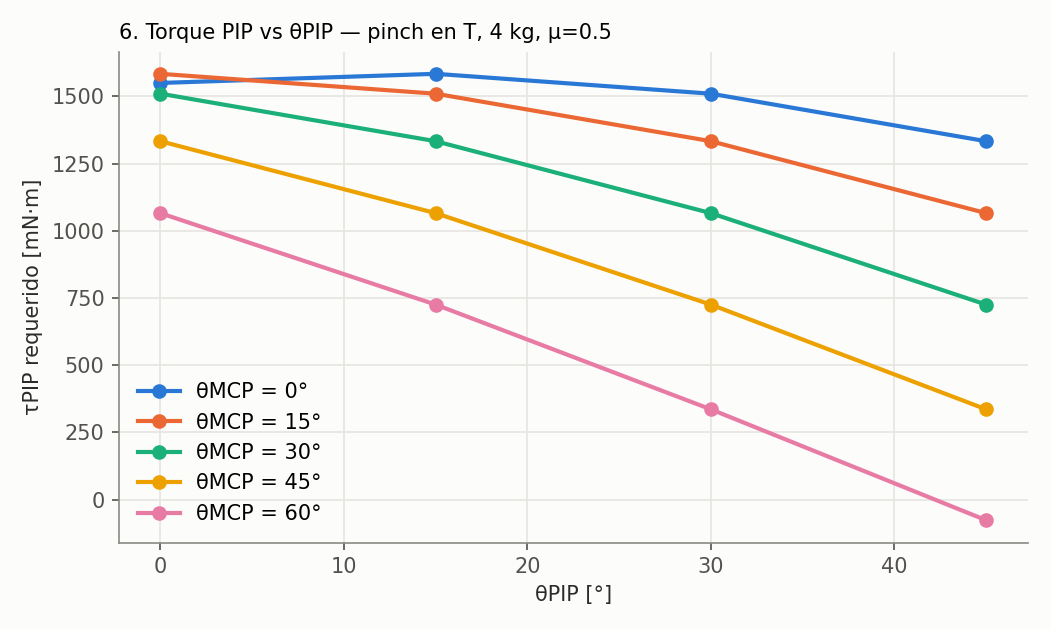
\includegraphics[width=0.8\textwidth]{06_tauPIP_vs_PIP.png}
\caption{Torque PIP requerido en pinch en la punta, 4 kg.}
\label{fig:g06}
\end{figure}
\par\noindent\textbf{Análisis.} El torque PIP baja casi linealmente al flexionar el PIP y se vuelve negativo con el MCP a 60°. El máximo, 1.58 N$\cdot$m, se da con el dedo casi recto; agarrar con el dedo más cerrado reduce mucho la carga del N20.


\begin{figure}[H]
\centering
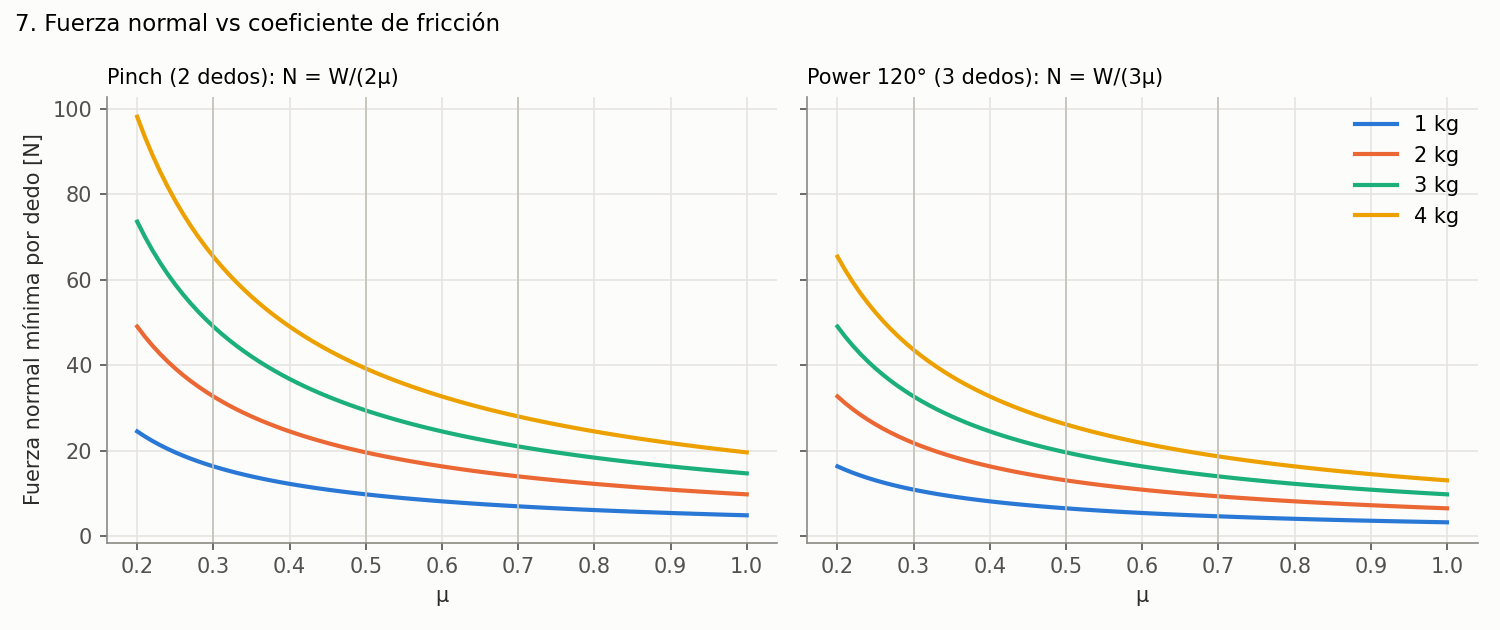
\includegraphics[width=1.0\textwidth]{07_N_vs_mu.png}
\caption{Fuerza normal mínima por dedo contra el coeficiente de fricción.}
\label{fig:g07}
\end{figure}
\par\noindent\textbf{Análisis.} La normal mínima es inversamente proporcional a $\mu$: pasar de $\mu$ = 0.3 a 0.7 la reduce a menos de la mitad (65.4 $\rightarrow$ 28.0 N en un pinch de 4 kg). El power a 120° necesita dos tercios de la normal del pinch porque reparte el peso entre tres dedos. Un recubrimiento de alta fricción en las yemas es la forma más directa de bajar todos los torques.


\begin{figure}[H]
\centering
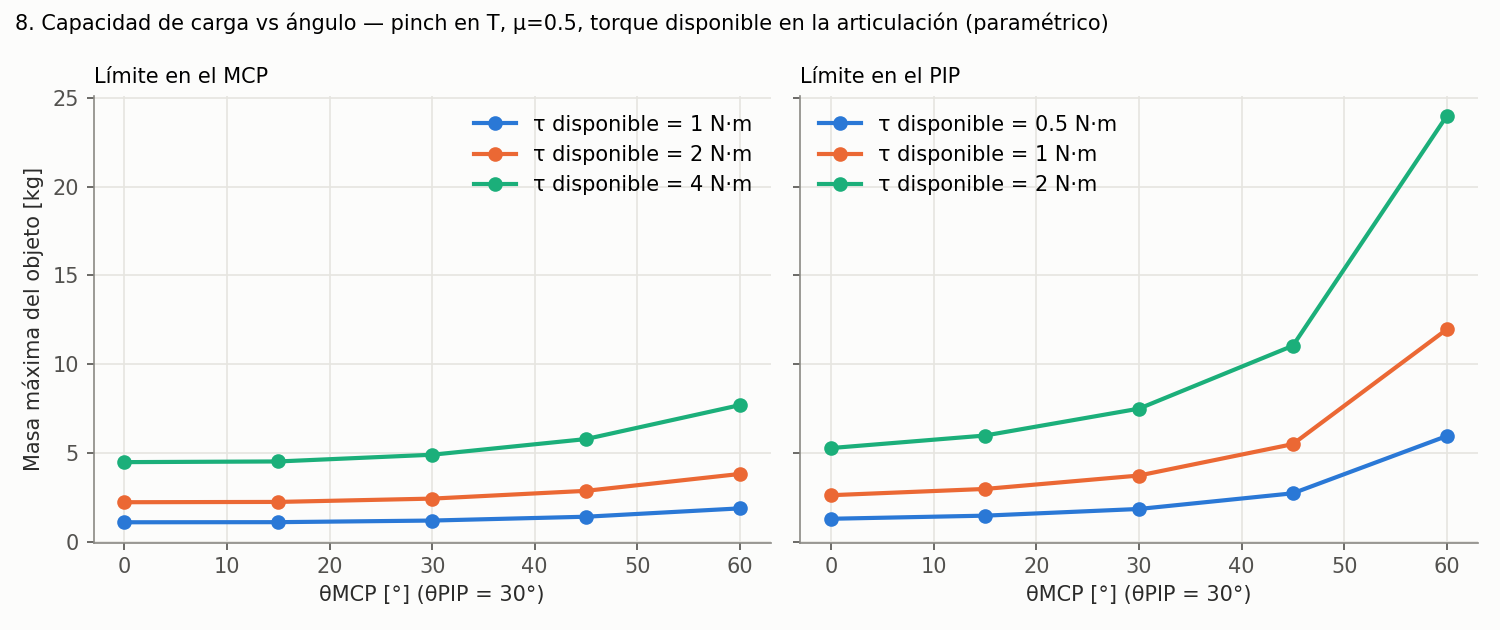
\includegraphics[width=1.0\textwidth]{08_capacidad_vs_angulo.png}
\caption{Masa máxima sostenible según el torque disponible en cada articulación.}
\label{fig:g08}
\end{figure}
\par\noindent\textbf{Análisis.} La capacidad aumenta al cerrar el MCP porque baja el torque requerido. El PIP limita más que el MCP: con 1 N$\cdot$m disponible en el PIP, un pinch en la punta con el dedo recto sostiene 2.65 kg, mientras que 2 N$\cdot$m en el MCP permiten 2.25 kg con el dedo recto y 3.84 kg con el MCP a 60°.


\begin{figure}[H]
\centering
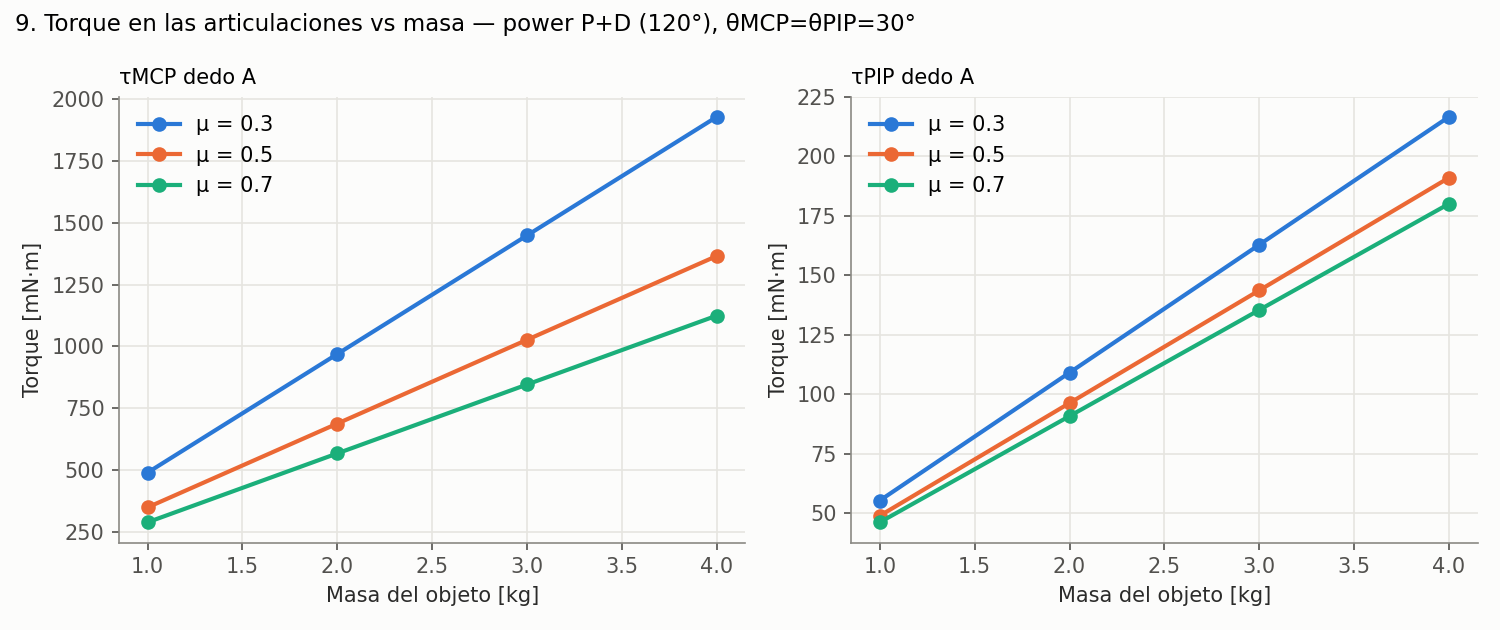
\includegraphics[width=1.0\textwidth]{09_torque_articular_vs_masa.png}
\caption{Torques en las articulaciones del dedo A contra la masa del objeto.}
\label{fig:g09}
\end{figure}
\par\noindent\textbf{Análisis.} Los torques crecen linealmente con la masa, como predice $N = W/(n\mu)$. La fricción pesa mucho más en el MCP (1.929 frente a 1.124 N$\cdot$m a 4 kg entre $\mu$ = 0.3 y 0.7) que en el PIP (0.217 frente a 0.180 N$\cdot$m), porque la normal actúa con un brazo mucho mayor respecto al MCP.


\begin{figure}[H]
\centering
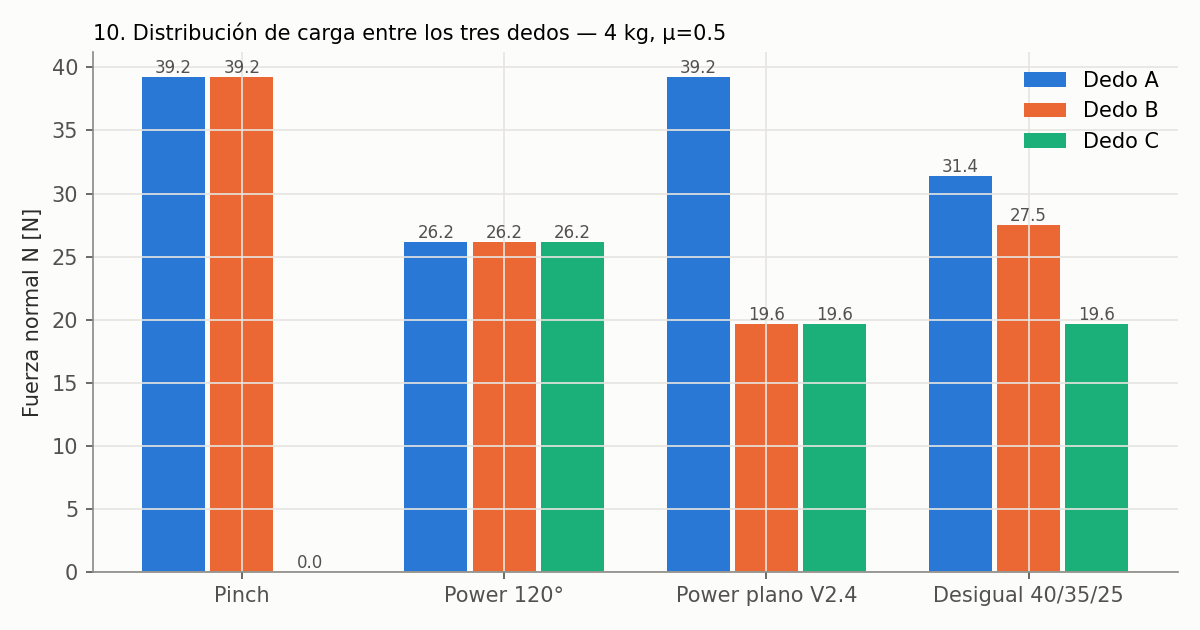
\includegraphics[width=0.85\textwidth]{10_distribucion_carga.png}
\caption{Distribución de la fuerza normal entre los tres dedos, 4 kg.}
\label{fig:g10}
\end{figure}
\par\noindent\textbf{Análisis.} La disposición del plano V2.4 hace que el dedo A cargue el doble que B y C (39.2 frente a 19.6 N), igual que en el pinch. El power a 120° es el reparto más equilibrado (26.2 N por dedo); por eso el dedo A y su N20 son los que deben dimensionarse para el peor caso.


% <<< graficas barrido
\subsection{Análisis de resultados estáticos}
\begin{itemize}
\item El contacto en la punta con dedos rectos y $\mu = 0.3$ es la condición más exigente: 5.832 N$\cdot$m en el MCP y 2.466 N$\cdot$m en el PIP con 4 kg. Agarrar en P o en P+D reduce el torque PIP hasta diez veces y el torque MCP a la mitad.
\item La normal de contacto aporta más del 90 \% de cada torque; el peso propio del dedo, menos del 0.5 \%.
\item Las reacciones en las articulaciones llegan a 68.4 N en el MCP y 68.3 N en el PIP, y son las cargas de entrada para el análisis de resistencia de materiales.
\item Los torques en las articulaciones son la base para seleccionar los actuadores; la relación de transmisión y su eficiencia se aplican después, en la etapa de selección.
\end{itemize}

% >>> caso 3.5 kg mu 0.3
\subsection{Caso de diseño 2: objeto de 3.5 kg y $\mu = 0.3$}
Los resultados anteriores usan como referencia un objeto de 4 kg con $\mu = 0.5$. En esta sección se repite el análisis con el caso de diseño actualizado, un objeto de 3.5 kg y un coeficiente de fricción de 0.3. Como en todo el análisis estático, no se considera el mecanismo ni la transmisión de engranajes: solo las medidas del dedo para obtener fuerzas y torques en cada punto de interés. Se sigue la metodología de análisis estático del curso: cuerpo rígido, diagrama de cuerpo libre con el tipo de apoyo de cada unión, equilibrio del sistema completo y de cada subensamble, escenarios críticos, y cargas internas por el método de las secciones.

\subsubsection{Metodología}
\begin{itemize}
\item \textbf{Cuerpo rígido.} Las falanges se consideran indeformables; el efecto del material se evalúa después en resistencia de materiales.
\item \textbf{Apoyos.} El MCP y el PIP son pasadores lisos con un actuador que fija el giro, por lo que cada uno aporta dos componentes de fuerza y un par (equivalente a un soporte fijo en 2D). El contacto con el objeto aporta una fuerza normal y una de fricción.
\item \textbf{Equilibrio por subensambles.} Se resuelve primero la falange distal, luego la proximal y por último la palma y la brida del UR5e. Las fuerzas en cada unión pasan de un subensamble al siguiente por acción-reacción:
\eq{\sum F_x = 0 \qquad \sum F_y = 0 \qquad \sum M_O = 0}
\item \textbf{Escenarios críticos.} Pinch en la punta, power a 120°, power con la disposición del plano y carga desigual, en 20 posturas y 3 puntos de contacto.
\item \textbf{Cargas internas.} En cada sección $s$ de una falange se suman las cargas que quedan del lado de la punta:
\eq{N(s) = \sum \vec F\cdot\hat u \qquad V(s) = \sum \vec F\cdot\hat n \qquad M(s) = \sum (\vec r_i - \vec r_s)\times\vec F_i}
\end{itemize}

La normal mínima $N = W/(n\mu)$ escala con $m/\mu$: frente al caso de referencia el factor es $(3.5/0.3)/(4/0.5) = 1.458$, es decir, la normal sube un 46 \% aunque la masa baje. La fricción que sostiene el peso, $F_t = W/n$, depende solo de la masa y baja un 12.5 \%. Como la normal domina el torque, los torques en las articulaciones suben entre un 23 y un 36 \% según la postura y el contacto.

\subsubsection{Resultados por caso}
\begin{table}[H]
\centering
\small
\begin{tabular}{|l|c|c|c|}
\hline
\rowcolor{head}\textbf{Caso (15°/15°)} & \textbf{N por dedo [N]} & \textbf{$\tau_{MCP}$ A / B / C [N$\cdot$m]} & \textbf{$\tau_{PIP}$ A / B / C [N$\cdot$m]} \\ \hline
Pinch (T) & 57.2 / 57.2 / 0 & 4.909 / 4.909 / 0.005 & 1.912 / 1.912 / 0.001 \\ \hline
Power 120° (D) & 38.2 / 38.2 / 38.2 & 2.749 / 2.749 / 2.749 & 0.750 / 0.750 / 0.750 \\ \hline
Power plano (D) & 57.2 / 28.6 / 28.6 & 4.121 / 2.063 / 2.063 & 1.124 / 0.563 / 0.563 \\ \hline
Desigual 40/35/25 (T) & 45.8 / 40.1 / 28.6 & 3.928 / 3.438 / 2.457 & 1.530 / 1.339 / 0.957 \\ \hline
\end{tabular}
\caption{Estática con 3.5 kg y $\mu = 0.3$ en la postura 15°/15°: fuerza normal y torques en las articulaciones de cada dedo. Con 4 kg y $\mu = 0.5$ el pinch daba 3.698 / 1.510 N$\cdot$m.}
\label{tab:caso35}
\end{table}

\begin{table}[H]
\centering
\small
\begin{tabular}{|l|c|c|}
\hline
\rowcolor{head}\textbf{Magnitud} & \textbf{4 kg, $\mu = 0.5$} & \textbf{3.5 kg, $\mu = 0.3$} \\ \hline
Normal por dedo en pinch & 39.2 N & 57.2 N \\ \hline
Peor torque en el MCP (pinch en T, 15°/0°) & 3.772 N$\cdot$m & 5.104 N$\cdot$m \\ \hline
Peor torque en el PIP (pinch en T, dedo recto) & 1.584 N$\cdot$m & 2.157 N$\cdot$m \\ \hline
Peor reacción en el MCP (pinch en P) & 44.1 N & 59.9 N \\ \hline
Vista superior: $N_A = N_B + N_C$ & 39.2 = 19.6 + 19.6 N & 57.2 = 28.6 + 28.6 N \\ \hline
Vista frontal: brida del UR5e & $F_z$ = 40.5 N, $M_y$ = 0.21 N$\cdot$m & $F_z$ = 35.6 N, $M_y$ = 0.18 N$\cdot$m \\ \hline
\end{tabular}
\caption{Comparación entre los dos casos de diseño.}
\label{tab:comp35}
\end{table}

\begin{figure}[H]
\centering
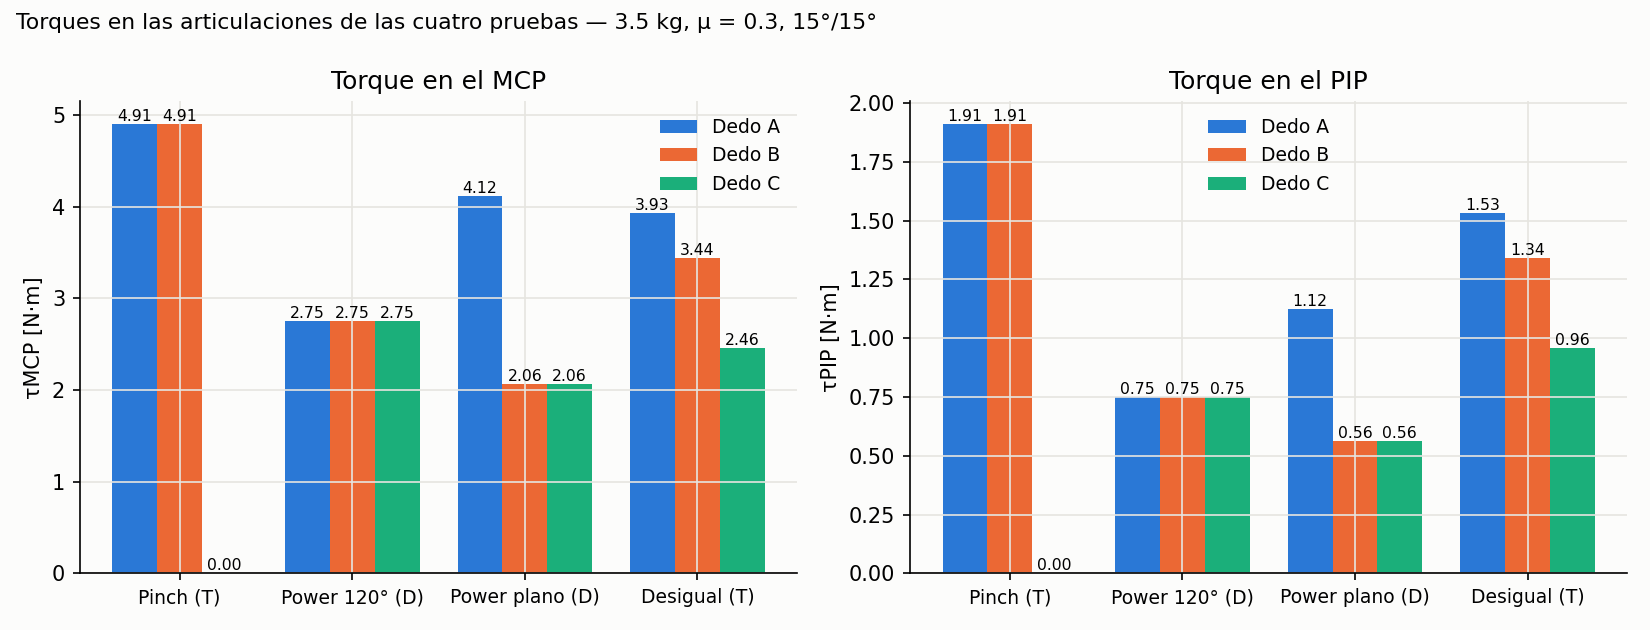
\includegraphics[width=\textwidth]{J3_torques_pruebas.png}
\caption{Torques en las articulaciones de cada dedo en las cuatro pruebas (3.5 kg, $\mu = 0.3$, 15°/15°).}
\label{fig:e1}
\end{figure}
\par\noindent\textbf{Análisis.} El pinch es el caso más exigente: 4.909 N$\cdot$m en el MCP y 1.912 N$\cdot$m en el PIP de los dedos A y B. El power a 120° reparte la carga por igual (2.749 / 0.750 N$\cdot$m por dedo), y en el power plano el dedo A carga el doble que B y C.

\begin{figure}[H]
\centering
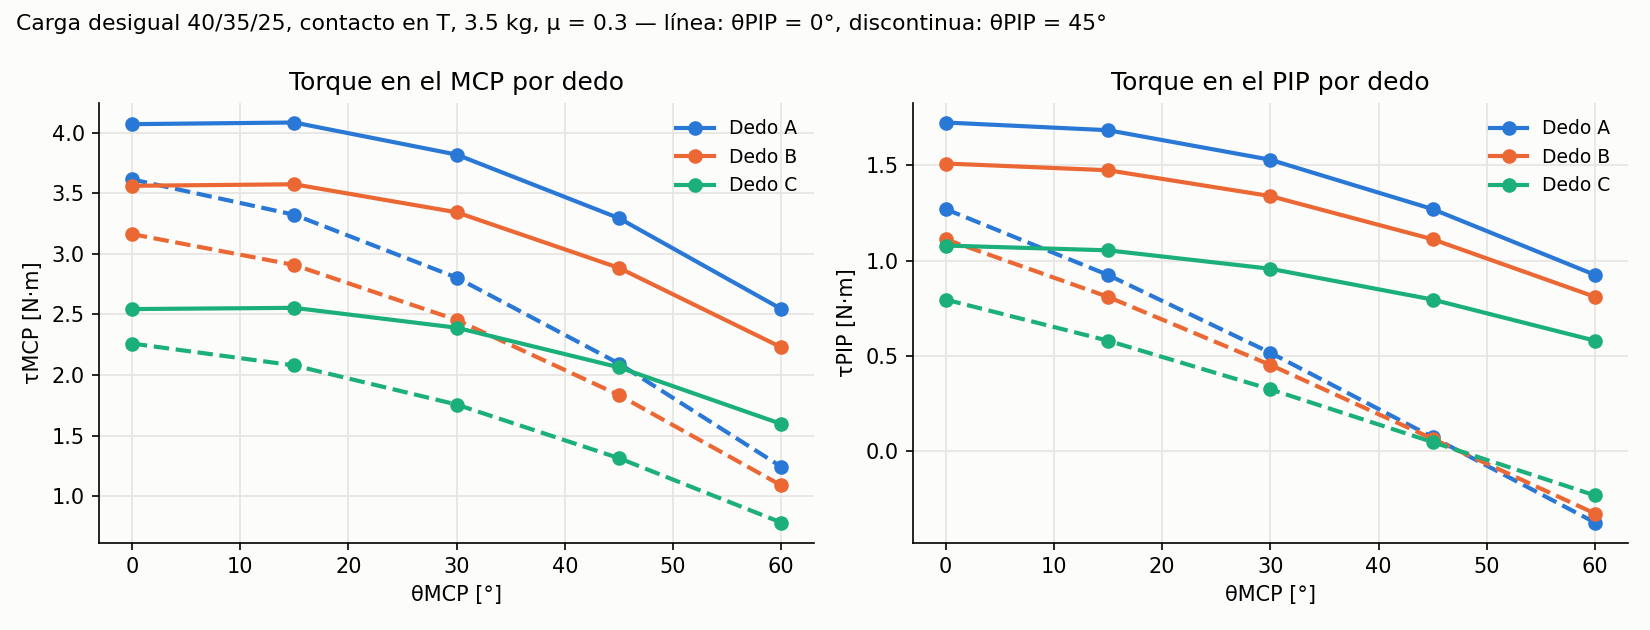
\includegraphics[width=\textwidth]{J1_torques_por_dedo.png}
\caption{Torques en el MCP y el PIP de cada dedo contra $\theta_{MCP}$ (carga desigual, contacto en T, 3.5 kg, $\mu = 0.3$).}
\label{fig:e2}
\end{figure}
\par\noindent\textbf{Análisis.} Los torques siguen el reparto de la carga y bajan al cerrar el dedo. Frente a 4 kg con $\mu = 0.5$ suben entre un 23 y un 33 \% en la postura 15°/15° (el MCP del pinch pasa de 3.698 a 4.909 N$\cdot$m): menos que el 46 \% de la normal, porque la fricción tangencial baja con la masa.

\subsubsection{Vistas lateral, superior y frontal}
\begin{figure}[H]
\centering
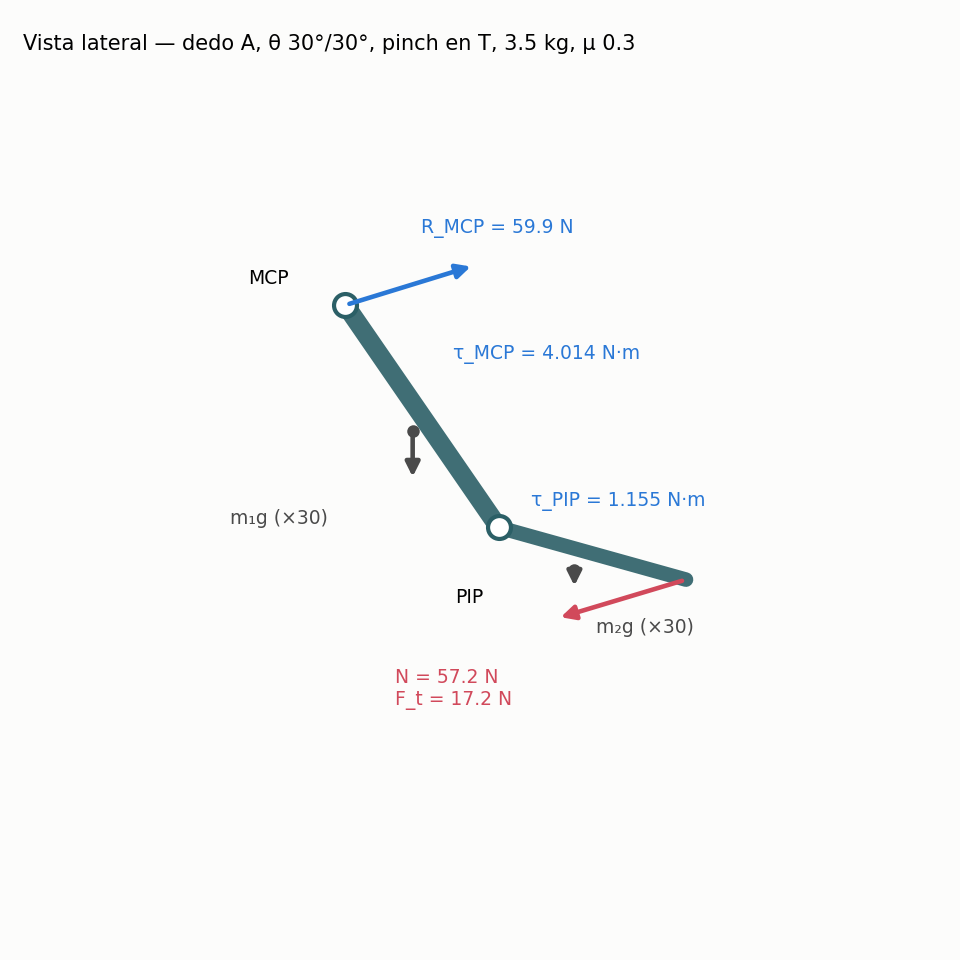
\includegraphics[width=0.55\textwidth]{D6_vista_lateral_DCL_35kg.png}
\caption{Diagrama de cuerpo libre en vista lateral del dedo A, 3.5 kg y $\mu = 0.3$.}
\label{fig:lateral35}
\end{figure}
\par\noindent\textbf{Análisis.} En un pinch de 3.5 kg en la punta con $\mu = 0.3$ la normal es $N = W/(2\mu) = 57.2$ N y la fricción $F_t = W/2 = 17.2$ N. El torque en el MCP es 4.014 N$\cdot$m y en el PIP 1.155 N$\cdot$m, con una reacción de 59.9 N en el MCP.

En la vista superior (Figura \ref{fig:superior35}) el dedo A está a 74.46 mm del par B--C, cuyos contactos están separados 34 mm. Con el origen en el contacto de A, B en $(74.46,\,17)$ mm, C en $(74.46,\,-17)$ mm y el centro del objeto a mitad de la distancia, las ecuaciones de equilibrio son:
\eq{\sum F_x = 0:\; N_A = N_B + N_C \qquad \sum M_z = 0:\; 17\,N_B - 17\,N_C = 0 \;\Rightarrow\; N_B = N_C}
Fuera del plano, la fricción de los tres contactos sostiene el peso:
\eq{\sum F_z = 0:\; f_A + f_B + f_C = W = 34.34 \text{ N} \qquad \sum M_x = 0:\; f_B = f_C}
\eq{\sum M_y = 0:\; 74.46\,(f_B + f_C) = 37.23\,W}
de donde $f_A = 17.17$ N y $f_B = f_C = 8.58$ N: el peso se reparte 50 / 25 / 25 \%. Con la condición de no deslizamiento $f_i \leq \mu N_i$, la fuerza de agarre mínima en cada dedo es:
\eq{N_A = \frac{f_A}{\mu} = \frac{W}{2\mu} = 57.2 \text{ N} \qquad N_B = N_C = \frac{W}{4\mu} = 28.6 \text{ N}}
lo que cumple $N_A = N_B + N_C$. La fuerza de agarre total es 114.5 N; con un factor de seguridad de 1.5 serían 85.9 N en A y 42.9 N en B y C.

\begin{figure}[H]
\centering
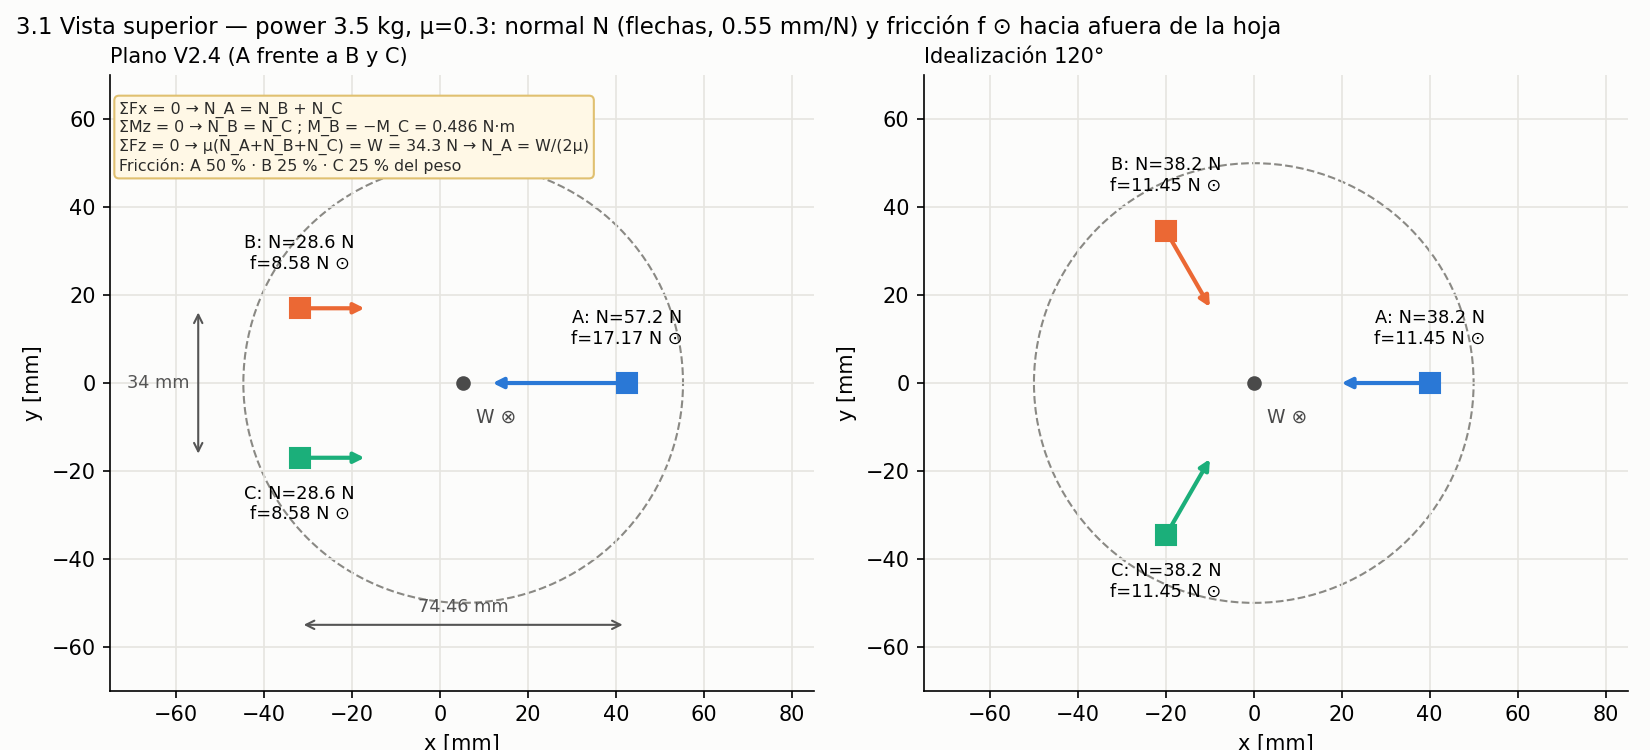
\includegraphics[width=\textwidth]{D5_vista_superior_35kg.png}
\caption{Vista superior con 3.5 kg y $\mu = 0.3$: normales en el plano y fricción hacia afuera de la hoja.}
\label{fig:superior35}
\end{figure}

\begin{table}[H]
\centering
\begin{tabular}{|l|c|c|c|}
\hline
\rowcolor{head}\textbf{Fuerza o momento} & \textbf{Dedo A} & \textbf{Dedo B} & \textbf{Dedo C} \\ \hline
Normal $N$ (fuerza de agarre) & 57.2 N & 28.6 N & 28.6 N \\ \hline
Fricción $f$ (hacia afuera de la hoja) & 17.17 N & 8.58 N & 8.58 N \\ \hline
Parte del peso & 50 \% & 25 \% & 25 \% \\ \hline
Momento de $N$ respecto al eje del objeto & 0 & +0.486 N$\cdot$m & $-$0.486 N$\cdot$m \\ \hline
Momento de $f$ respecto al eje $y$ del objeto & 0.639 N$\cdot$m & \multicolumn{2}{c|}{0.639 N$\cdot$m (B + C)} \\ \hline
\end{tabular}
\caption{Fuerzas y momentos de la vista superior con 3.5 kg y $\mu = 0.3$.}
\label{tab:superior35}
\end{table}
\par\noindent\textbf{Análisis.} Los momentos de B y C respecto al eje del objeto (±0.486 N$\cdot$m) se anulan solo si los dos dedos aprietan igual; cualquier diferencia hace girar el objeto en el plano de la palma. Los momentos de la fricción de A y del par B--C (0.639 N$\cdot$m cada uno) también se equilibran. Si el centro del objeto no queda a mitad de los 74.46 mm, el reparto 50 / 25 / 25 \% cambia y con él las fuerzas de agarre.

\begin{figure}[H]
\centering
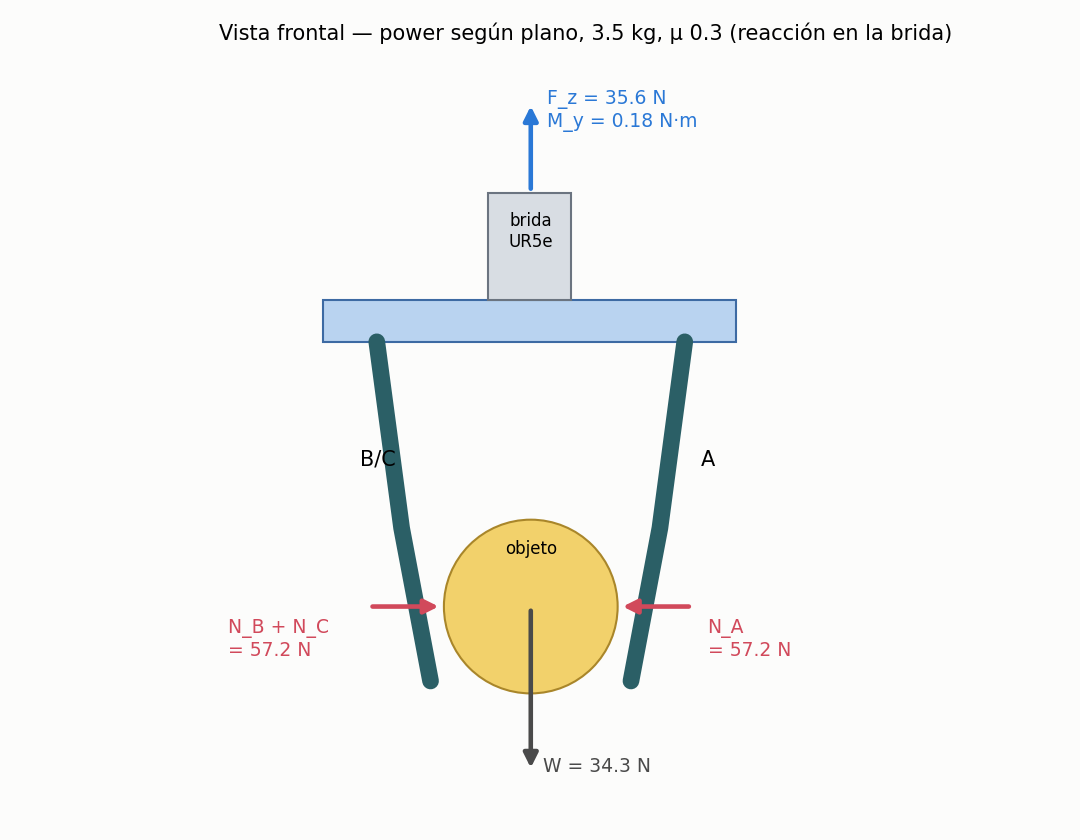
\includegraphics[width=0.62\textwidth]{D7_vista_frontal_DCL_35kg.png}
\caption{Diagrama de cuerpo libre en vista frontal con 3.5 kg y $\mu = 0.3$.}
\label{fig:frontal35}
\end{figure}
\par\noindent\textbf{Análisis.} La brida del UR5e soporta $F_z = 35.6$ N (los 34.3 N del objeto más el peso de los dedos) y un momento $M_y = 0.18$ N$\cdot$m por la excentricidad de 5.27 mm del eje del objeto respecto al eje del gripper.

\subsubsection{Estática del dedo por tipo de agarre}
Los tres dedos son iguales, así que se analiza un solo dedo en vista lateral con las cargas de cada uno obtenidas en la vista superior: el dedo solo (A) recibe $N = W/(2\mu) = 57.23$ N y $f = W/2 = 17.17$ N, y cada dedo del par (B o C) la mitad, $N = 28.61$ N y $f = 8.58$ N. El análisis no considera el mecanismo ni la transmisión de engranajes: solo usa las medidas del dedo recto para obtener las fuerzas y los torques en cada punto de interés (P, D, PIP y MCP).

Con el origen en el MCP, $y'$ a lo largo del dedo y $z'$ hacia el dorso, las medidas usadas son:
\eq{r_2 = \overrightarrow{MCP\,P} = (31,\,-13) \qquad r_3 = \overrightarrow{MCP\,PIP} = (50,\,-4) \qquad r_9 = \overrightarrow{PIP\,D} = (21.45,\,-9) \text{ mm}}
de modo que el contacto D queda en $r_3 + r_9 = (71.45,\,-13)$ mm desde el MCP. La normal empuja el dedo hacia el dorso ($+z'$) y la fricción actúa a lo largo del dedo hacia la punta ($+y'$). El momento de cada fuerza y el equilibrio de cada falange son:
\eq{M = y\,F_z - z\,F_y \qquad \vec R = -\sum \vec F}
\eq{\sum M_{PIP} = 0 \Rightarrow \tau_{PIP} = M_D^{PIP} \qquad \sum M_{MCP} = 0 \Rightarrow \tau_{MCP} = M_P^{MCP} + M_D^{MCP}}
En el pinch toda la carga va en D; en el power se reparte 50 / 50 entre P y D.

\begin{figure}[H]
\centering
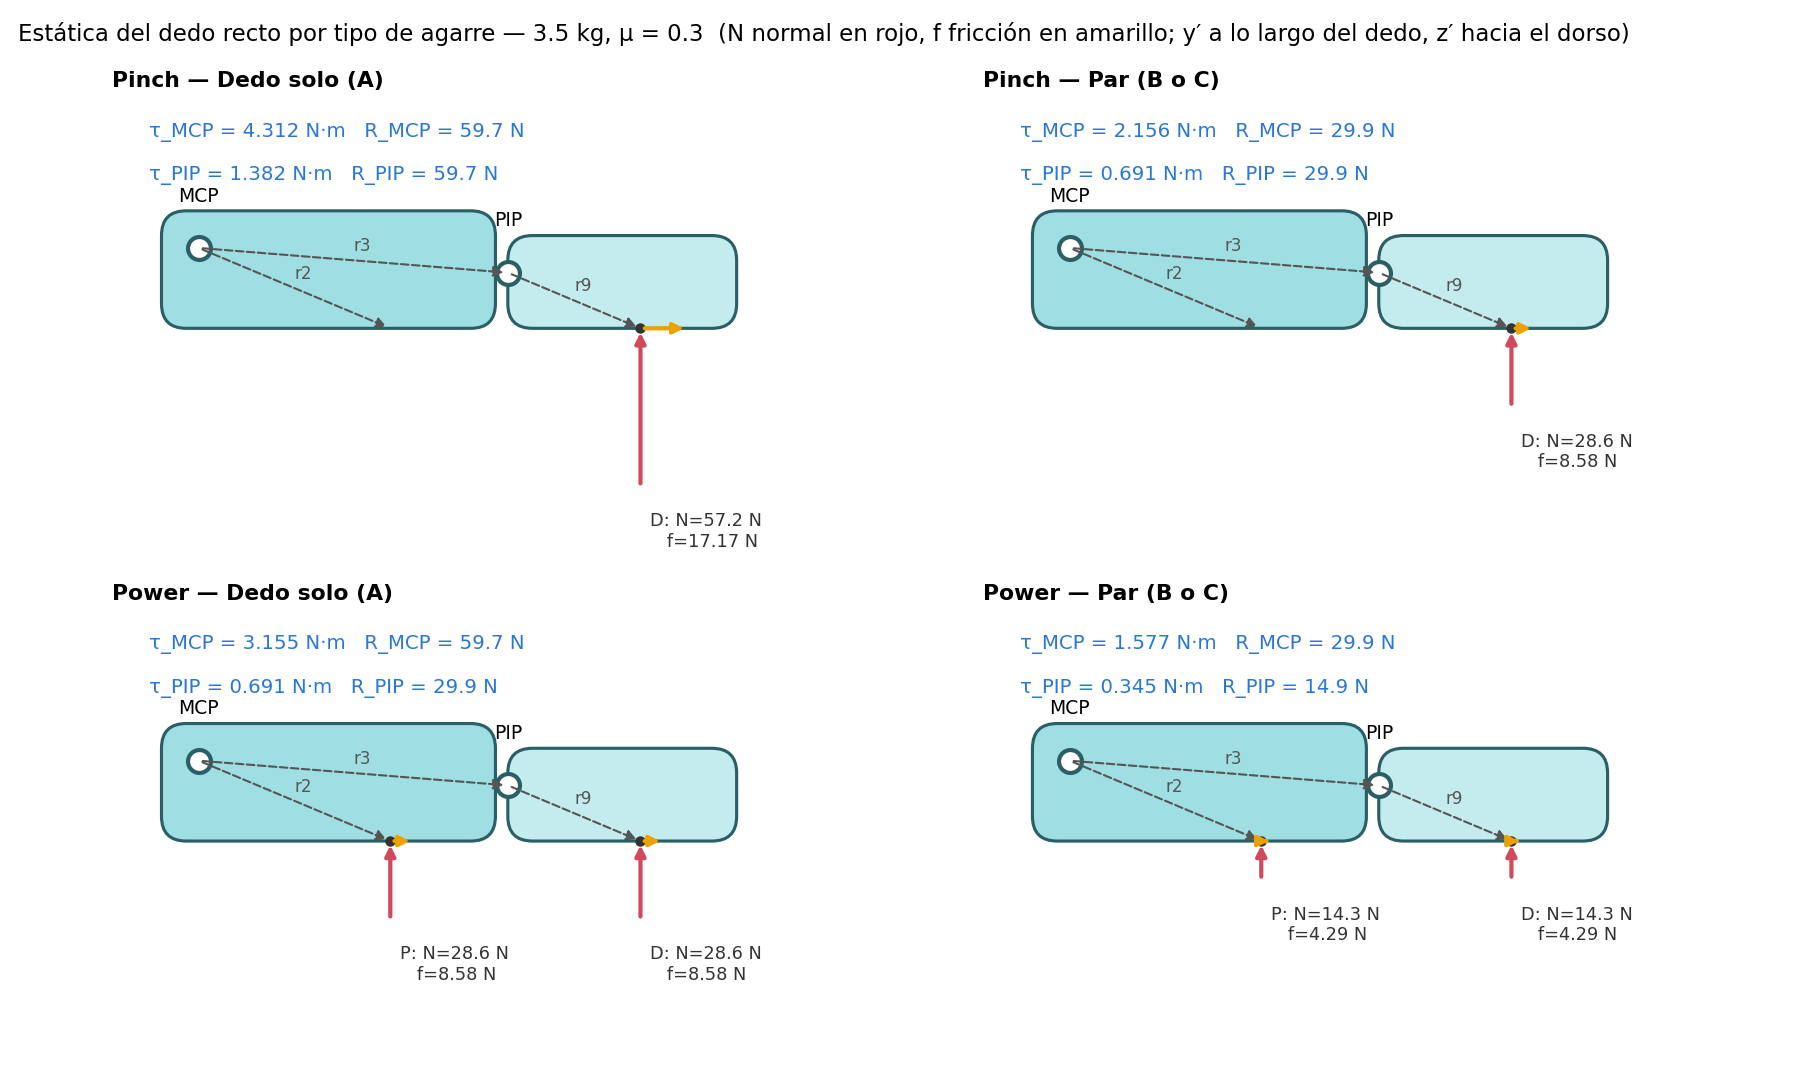
\includegraphics[width=\textwidth]{E5_dedo_agarres.png}
\caption{Diagrama de cuerpo libre del dedo recto en los cuatro casos de agarre (3.5 kg, $\mu = 0.3$).}
\label{fig:e5}
\end{figure}

\begin{table}[H]
\centering
\small
\begin{tabular}{|l|c|c|c|c|c|c|}
\hline
\rowcolor{head}\textbf{Caso} & \textbf{Carga en P} & \textbf{Carga en D} & \textbf{$\tau_{PIP}$ [N$\cdot$m]} & \textbf{$\tau_{MCP}$ [N$\cdot$m]} & \textbf{$R_{PIP}$} & \textbf{$R_{MCP}$} \\ \hline
Pinch, dedo solo & -- & 57.2 / 17.2 N & \textbf{1.382} & \textbf{4.312} & 59.7 N & 59.7 N \\ \hline
Pinch, par & -- & 28.6 / 8.6 N & 0.691 & 2.156 & 29.9 N & 29.9 N \\ \hline
Power, dedo solo & 28.6 / 8.6 N & 28.6 / 8.6 N & 0.691 & 3.155 & 29.9 N & 59.7 N \\ \hline
Power, par & 14.3 / 4.3 N & 14.3 / 4.3 N & 0.345 & 1.577 & 14.9 N & 29.9 N \\ \hline
\end{tabular}
\caption{Fuerzas (normal / fricción) y torques en las articulaciones del dedo recto, sin transmisión.}
\label{tab:dedo35}
\end{table}

En el pinch del dedo solo, por ejemplo, $\tau_{PIP} = 21.45(57.23) + 9(17.17) = 1.228 + 0.155 = 1.382$ N$\cdot$m y $\tau_{MCP} = 71.45(57.23) + 13(17.17) = 4.089 + 0.223 = 4.312$ N$\cdot$m. En el power del dedo solo el contacto P aporta $31(28.61) + 13(8.58) = 0.999$ N$\cdot$m al MCP y el contacto D $2.156$ N$\cdot$m, para un total de 3.155 N$\cdot$m.

\par\noindent\textbf{Análisis.} El caso que dimensiona es el pinch del dedo solo: 4.312 N$\cdot$m en el MCP y 1.382 N$\cdot$m en el PIP, con reacciones de 59.7 N en ambas articulaciones. La normal aporta más del 90 \% de cada torque; la fricción solo actúa con el brazo vertical de 9 a 13 mm. Pasar al power acerca parte de la carga al MCP y reduce el torque del MCP un 27 \% y el del PIP un 50 \%. Los dedos del par necesitan la mitad que el dedo solo en todos los casos. Estos torques en las articulaciones son la base para seleccionar los actuadores.

\subsubsection{Cargas internas}
\begin{figure}[H]
\centering
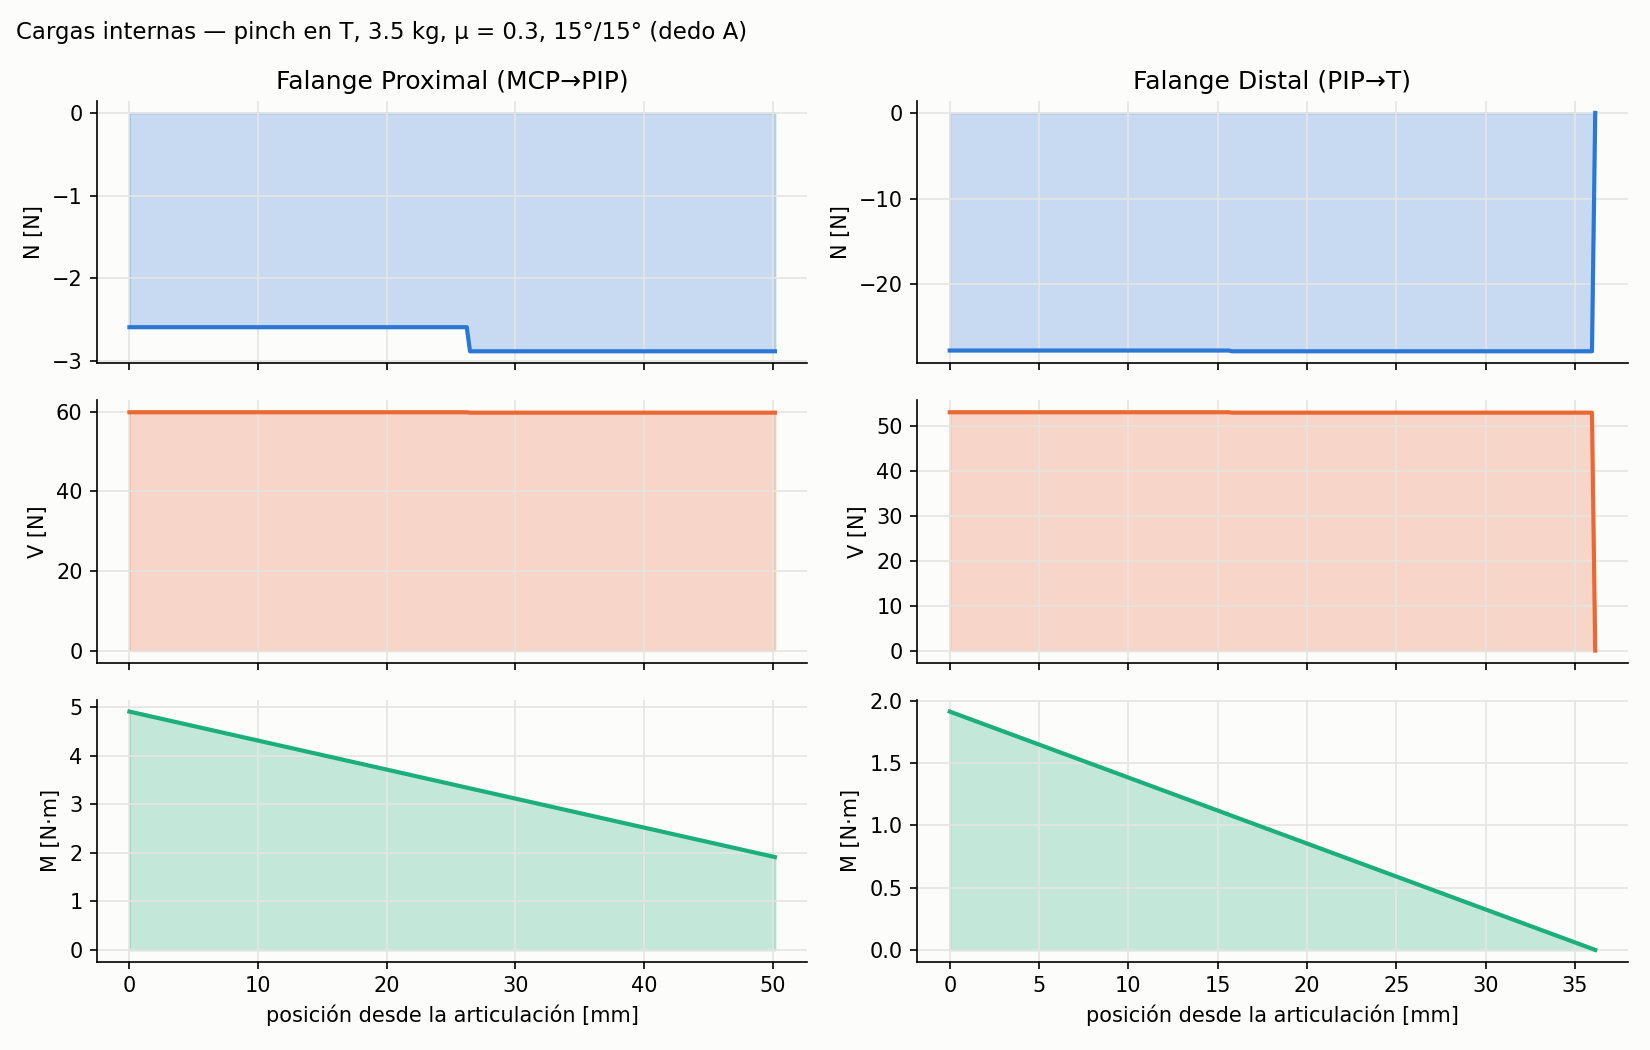
\includegraphics[width=\textwidth]{E3_cargas_internas.png}
\caption{Fuerza normal, cortante y momento flector a lo largo de cada falange (pinch en la punta, dedo A).}
\label{fig:e3}
\end{figure}
\par\noindent\textbf{Análisis.} Cada falange trabaja como una viga empotrada en su articulación y cargada en el contacto. El momento flector crece linealmente hacia la articulación: 4.91 N$\cdot$m en la raíz de la falange proximal y 1.91 N$\cdot$m en la raíz de la distal, iguales a $\tau_{MCP}$ y $\tau_{PIP}$, lo que verifica el equilibrio. La cortante es casi constante (59.8 N y 53.0 N) y la normal es de compresión (2.9 N y 27.8 N). La sección crítica es la raíz de la falange proximal y estas cargas son la entrada del análisis de resistencia de materiales.

\begin{figure}[H]
\centering
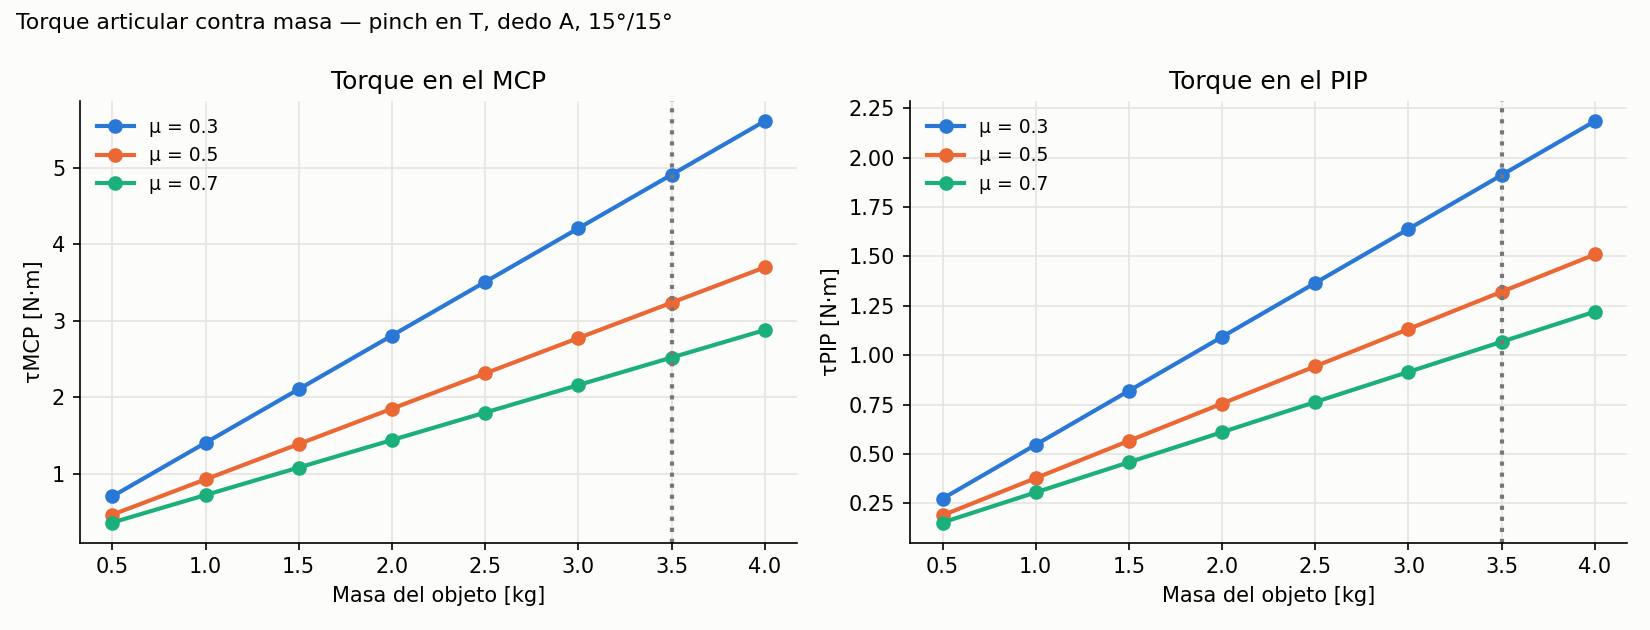
\includegraphics[width=\textwidth]{J2_torque_vs_masa.png}
\caption{Torques en el MCP y el PIP del dedo A contra la masa del objeto, para $\mu$ = 0.3, 0.5 y 0.7 (pinch en T, 15°/15°).}
\label{fig:e4}
\end{figure}
\par\noindent\textbf{Análisis.} Los torques crecen linealmente con la masa. Con 3.5 kg el MCP del dedo A necesita 4.91 N$\cdot$m con $\mu = 0.3$ y 3.23 N$\cdot$m con $\mu = 0.5$: aumentar la fricción de las yemas es la forma más directa de reducir todos los torques.

\subsubsection{Validación en Working Model 2D}
El modelo estático de Working Model se ejecutó con los deslizadores en 3.5 kg y $\mu = 0.3$ y se repitió el barrido de 180 configuraciones (3 casos $\times$ 3 contactos $\times$ 20 posturas). La diferencia máxima con el cálculo analítico fue de 0.034 \% y la media de 0.006 \%.

\begin{figure}[H]
\centering
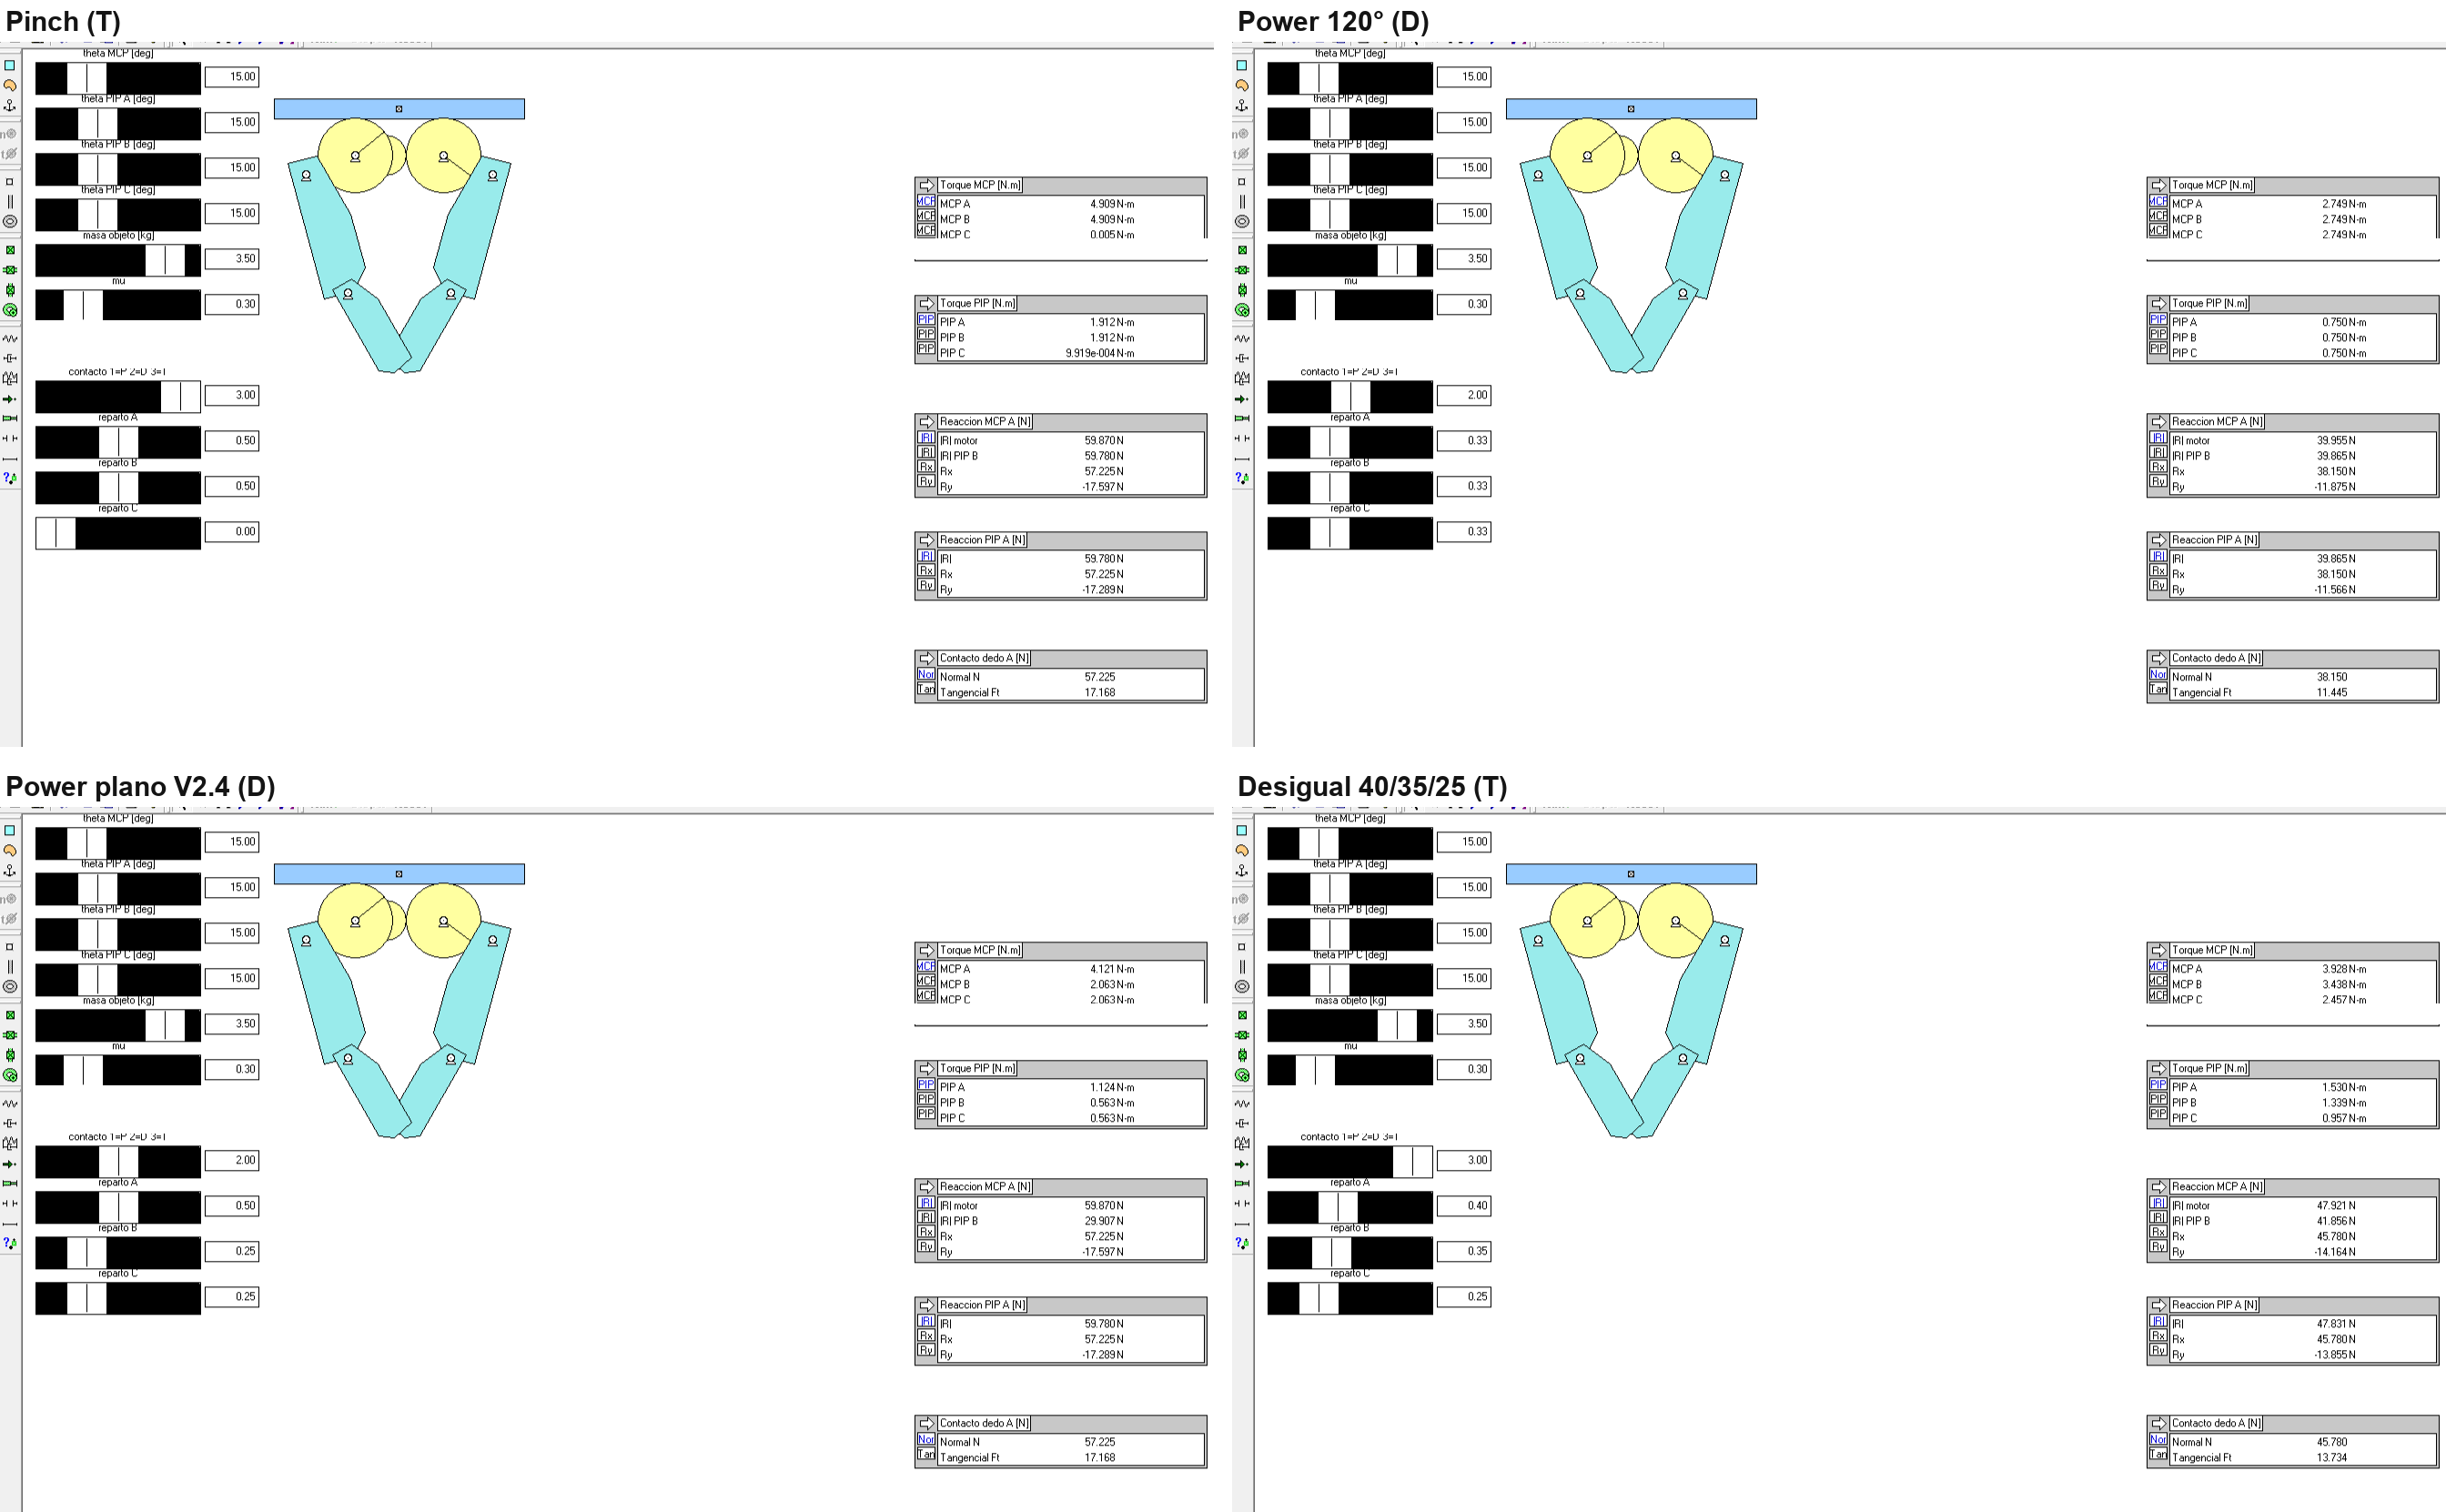
\includegraphics[width=\textwidth]{wm_pruebas_35kg_mu03.png}
\caption{Pruebas en Working Model 2D con 3.5 kg, $\mu = 0.3$ y postura 15°/15°.}
\label{fig:wm35}
\end{figure}
\par\noindent\textbf{Análisis.} Los medidores de Working Model reproducen los valores de la Tabla \ref{tab:caso35}: en el pinch los medidores marcan 4.909 N$\cdot$m en el MCP, 1.912 N$\cdot$m en el PIP y 57.2 N de normal; en el power plano el dedo A recibe 57.2 N y B y C 28.6 N cada uno.

\subsubsection{Análisis del caso de diseño 2}
\begin{itemize}
\item Bajar la fricción de 0.5 a 0.3 pesa más que bajar la masa de 4 a 3.5 kg: la normal de contacto sube un 46 \% y los torques en las articulaciones entre un 23 y un 36 \%.
\item El caso crítico es el pinch en la punta con el dedo casi recto: 5.104 N$\cdot$m en el MCP y 2.157 N$\cdot$m en el PIP.
\item En la estática del dedo recto con contacto en D, el dedo solo necesita 4.312 N$\cdot$m en el MCP y 1.382 N$\cdot$m en el PIP; cada dedo del par, la mitad.
\item La raíz de la falange proximal soporta 4.91 N$\cdot$m de flexión y 59.8 N de cortante; estos valores definen el dimensionamiento estructural.
\end{itemize}
% <<< caso 3.5 kg mu 0.3

% ======================================================================
\section{Cálculos cinemáticos (3.3)}
\subsection{Descripción}
El análisis cinemático describe los desplazamientos, velocidades y aceleraciones lineales y angulares de las falanges durante el cierre. Como el plano no define la velocidad del servo ni la del N20, el cierre se modela con una ley de movimiento cicloidal de duración $t_c$, que parte y termina con velocidad y aceleración nulas, y se reporta cómo escalan los resultados con $t_c$.

\subsection{Objetivo de cálculo}
\begin{itemize}
\item Determinar la evolución de $\theta$, $\omega$ y $\alpha$ de cada articulación y de la falange distal.
\item Calcular el desplazamiento, la velocidad y la aceleración lineal de los puntos de contacto P, D y T, del eje PIP y de los centros de masa.
\item Obtener las velocidades requeridas en los ejes de los motores y en los engranes.
\end{itemize}

\subsection{Modelo de cálculo}
La ley cicloidal para un recorrido $h$ en un tiempo $t_c$ es:
\eq{\theta(t) = h\left(\frac{t}{t_c} - \frac{1}{2\pi}\sin\frac{2\pi t}{t_c}\right) \qquad \omega(t) = \frac{h}{t_c}\left(1-\cos\frac{2\pi t}{t_c}\right) \qquad \alpha(t) = \frac{2\pi h}{t_c^2}\sin\frac{2\pi t}{t_c}}

La velocidad de cualquier punto se obtiene con el Jacobiano del dedo y la aceleración derivando nuevamente:
\eq{\dot{\mathbf{x}}_T = \mathbf{J}(\theta)\,\dot{\boldsymbol\theta} \qquad \ddot{\mathbf{x}}_T = \mathbf{J}(\theta)\,\ddot{\boldsymbol\theta} + \dot{\mathbf{J}}(\theta)\,\dot{\boldsymbol\theta}}

Las velocidades de los motores se obtienen con las relaciones de transmisión: $\omega_{sinfín} = 12\,\omega_{MCP}$ y $\omega_{N20} = 4\,\omega_{PIP}$.

La Figura \ref{fig:diagcin} muestra las variables cinemáticas sobre el dedo en un instante del cierre: los ángulos articulares, las velocidades y aceleraciones angulares y los vectores de velocidad de P, D y T y de aceleración de la punta.

\begin{figure}[H]
\centering
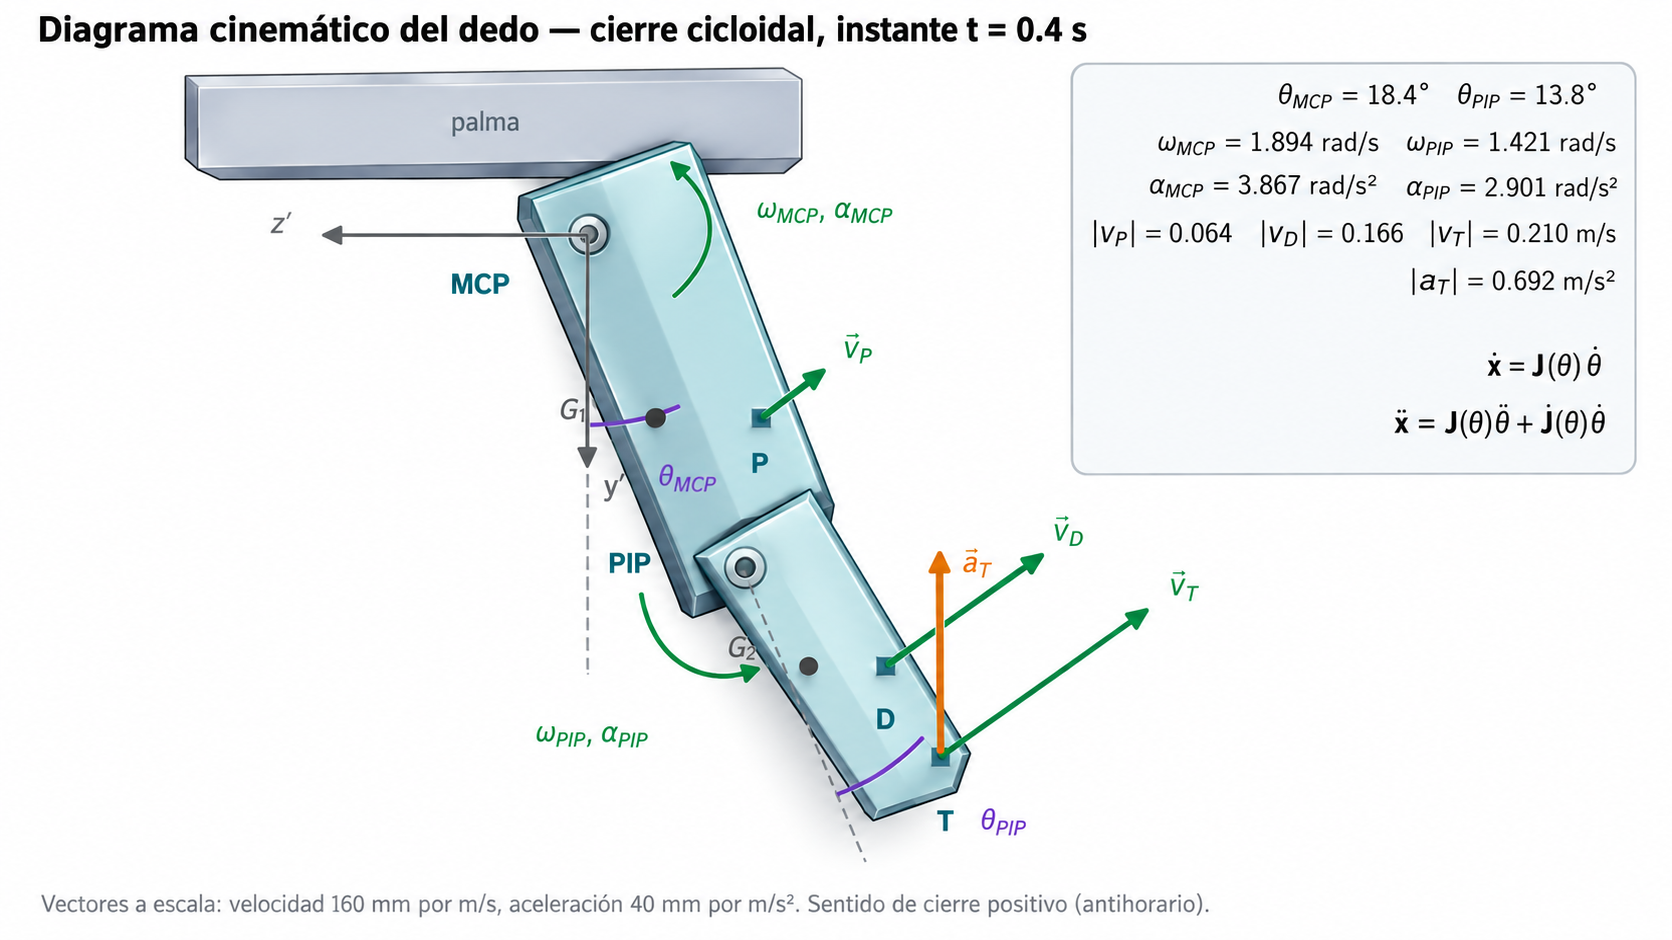
\includegraphics[width=\textwidth]{D9_diagrama_cinematico_chatgpt.png}
\caption{Diagrama cinemático del dedo en $t = 0.4$ s del cierre cicloidal. Diagrama generado con el modelo y mejorado gráficamente con IA; los valores se verificaron contra el cálculo.}
\label{fig:diagcin}
\end{figure}
\par\noindent\textbf{Análisis.} En t = 0.4 s el dedo ha cerrado 18.4° en el MCP y 13.8° en el PIP, y las dos articulaciones giran en el sentido de cierre (1.894 y 1.421 rad/s) mientras todavía aceleran (3.867 y 2.901 rad/s$^2$). La velocidad crece con la distancia a las articulaciones: 0.064 m/s en P, 0.166 m/s en D y 0.210 m/s en la punta. La aceleración de la punta (0.692 m/s$^2$) apunta hacia la palma porque suma las componentes tangenciales ($\alpha r$) y centrípetas ($\omega^2 r$) de los dos giros.


\subsection{Valores del modelo de cálculo}
Se considera un cierre de $0°$ a $60°$ en el MCP y de $0°$ a $45°$ en el PIP en $t_c = 1$ s (dato faltante: velocidad real de los motores).

\subsection{Resultados}
\begin{figure}[H]
\centering
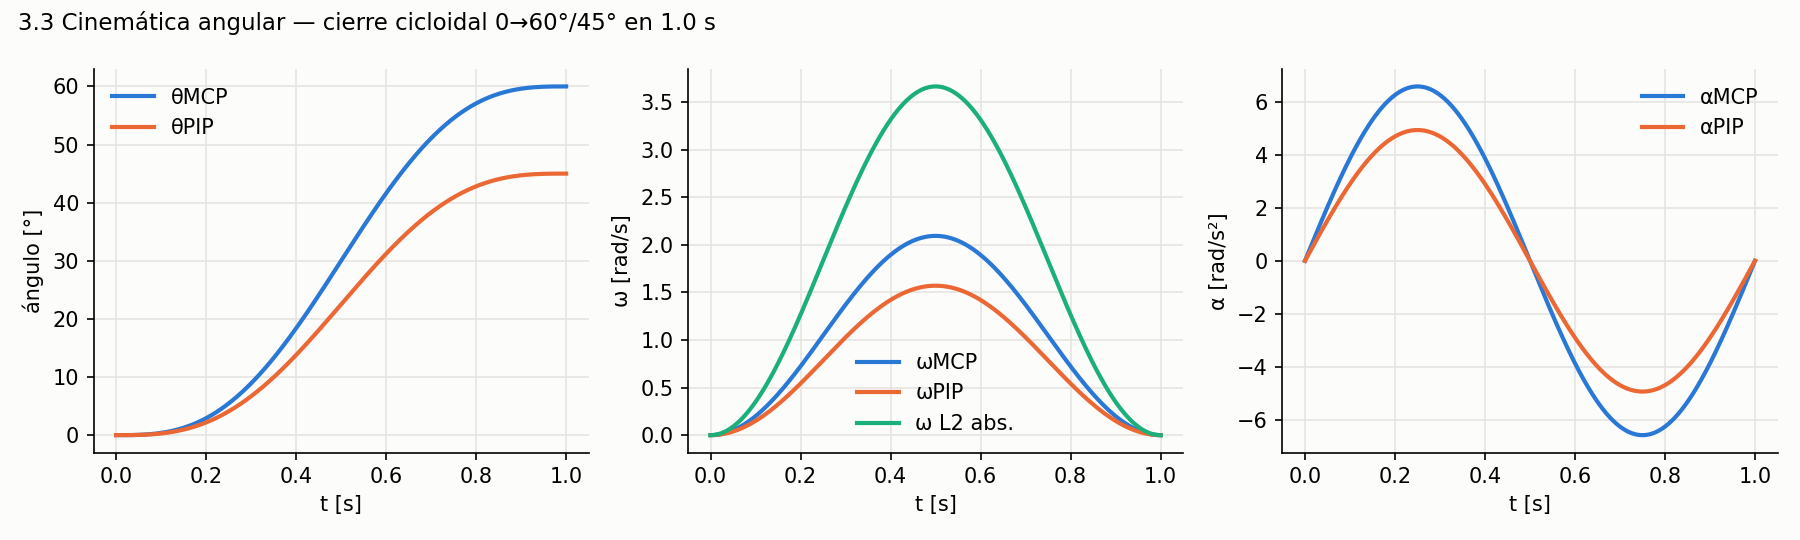
\includegraphics[width=\textwidth]{D1_cinematica_angular.png}
\caption{Posición, velocidad y aceleración angular durante el cierre.}
\label{fig:cinang}
\end{figure}
\par\noindent\textbf{Análisis.} El perfil cicloidal arranca y termina con velocidad y aceleración nulas, lo que evita impactos en los engranes. La velocidad máxima ocurre a mitad del cierre (2.094 rad/s en el MCP y 1.571 rad/s en el PIP) y las aceleraciones máximas a un cuarto y a tres cuartos del recorrido (6.58 y 4.94 rad/s$^2$). La falange distal suma ambos giros y alcanza 3.67 rad/s.




\begin{figure}[H]
\centering
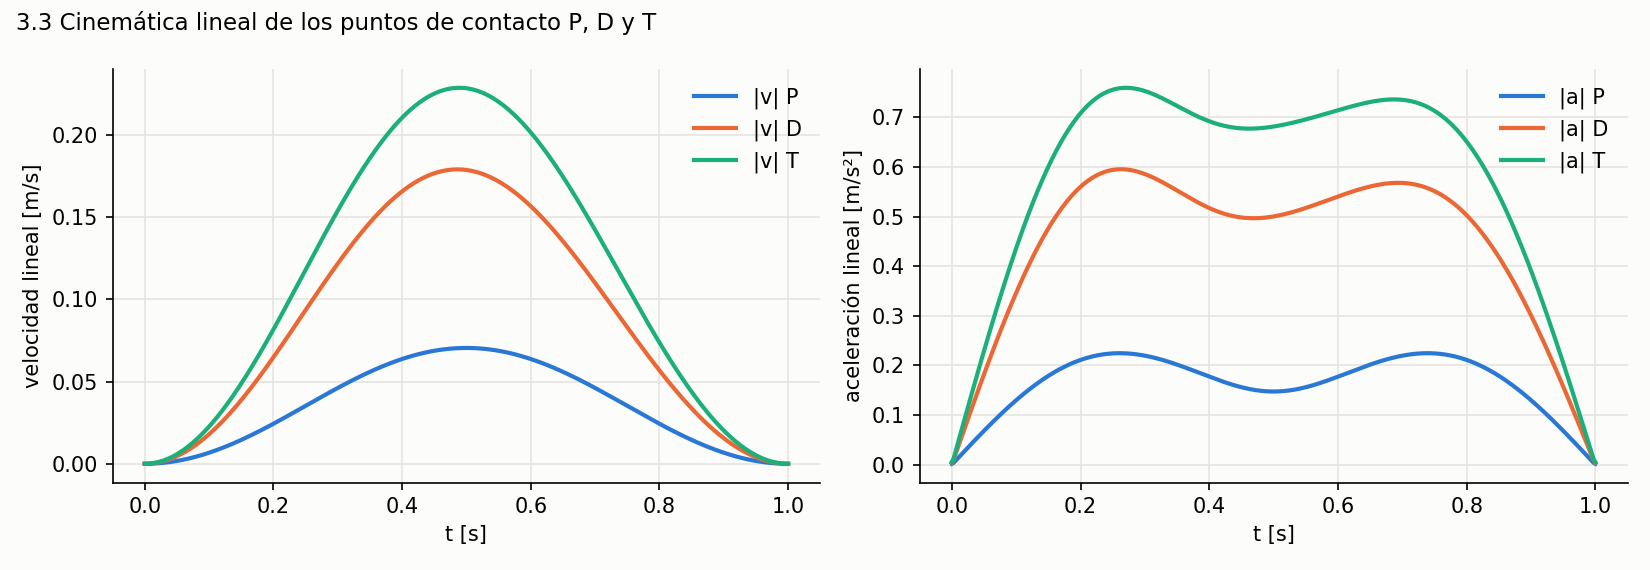
\includegraphics[width=\textwidth]{D2_cinematica_lineal.png}
\caption{Velocidad y aceleración lineal de los puntos de contacto.}
\label{fig:cinlin}
\end{figure}
\par\noindent\textbf{Análisis.} La punta T es el punto más rápido (0.229 m/s y 0.760 m/s$^2$) porque es el más alejado de las articulaciones; D llega a 0.179 m/s y P a 0.070 m/s. Las curvas tienen la misma forma de campana que el perfil angular, así que las velocidades escalan con $1/t_c$ y las aceleraciones con $1/t_c^2$.




\begin{figure}[H]
\centering
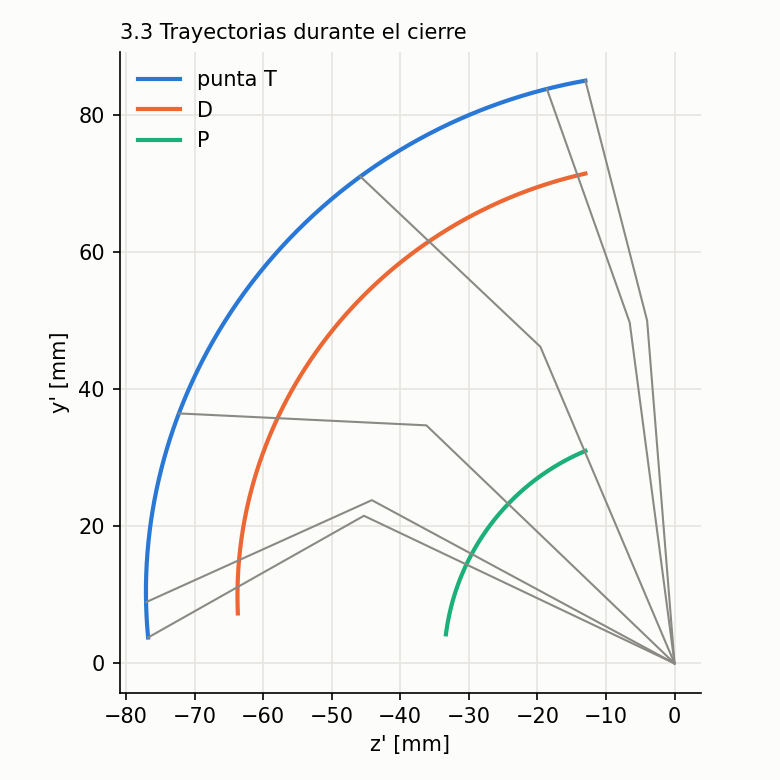
\includegraphics[width=0.55\textwidth]{D3_trayectorias.png}
\caption{Trayectorias de P, D y T y posturas intermedias del dedo.}
\label{fig:tray}
\end{figure}
\par\noindent\textbf{Análisis.} Las posturas intermedias muestran cómo se enrolla el dedo: la falange distal gira 105° en total frente a 60° de la proximal. Por eso la punta recorre 113.4 mm, más del triple que el contacto P (35.2 mm), y es la que primero toca objetos pequeños.




La Tabla \ref{tab:desplaz} resume los desplazamientos lineales: posición inicial y final de cada punto en el marco del dedo, componentes del desplazamiento, cuerda $|\Delta r|$ y longitud del recorrido curvo. La Tabla \ref{tab:desplazang} da los desplazamientos angulares de las falanges y del tren de transmisión.

\begin{table}[H]
\centering

\begin{adjustbox}{max width=\textwidth}
\begin{tabular}{|l|c|c|r|r|r|r|r|r|}
\hline
\textbf{Punto} & \textbf{Inicial $(y', z')$ [mm]} & \textbf{Final $(y', z')$ [mm]} & \textbf{$\Delta y'$ [mm]} & \textbf{$\Delta z'$ [mm]} & \textbf{$|\Delta r|$ [mm]} & \textbf{Recorrido [mm]} & \textbf{$|v|$ máx. [m/s]} & \textbf{$|a|$ máx. [m/s$^2$]} \\ \hline
P (falange proximal) & (31.0, -13.0) & (4.2, -33.3) & -26.8 & -20.3 & 33.6 & 35.2 & 0.070 & 0.225 \\ \hline
Eje PIP & (50.0, -4.0) & (21.5, -45.3) & -28.5 & -41.3 & 50.2 & 52.5 & 0.105 & 0.335 \\ \hline
D (falange distal) & (71.5, -13.0) & (7.3, -63.7) & -64.2 & -50.7 & 81.8 & 88.7 & 0.179 & 0.595 \\ \hline
T (punta) & (85.0, -13.0) & (3.8, -76.8) & -81.2 & -63.8 & 103.3 & 113.4 & 0.229 & 0.760 \\ \hline
$G_1$ (c.m. proximal) & (26.5, 0.9) & (14.0, -22.5) & -12.5 & -23.4 & 26.5 & 27.8 & 0.056 & 0.177 \\ \hline
$G_2$ (c.m. distal) & (66.2, -4.1) & (17.2, -60.9) & -49.0 & -56.8 & 75.0 & 80.8 & 0.163 & 0.530 \\ \hline
\end{tabular}
\end{adjustbox}
\caption{Desplazamientos lineales de los puntos del dedo en el cierre $0 \rightarrow 60°/45°$ ($t_c = 1$ s).}
\label{tab:desplaz}
\end{table}
\begin{table}[H]
\centering

\begin{adjustbox}{max width=\textwidth}
\begin{tabular}{|l|r|r|r|}
\hline
\textbf{Elemento} & \textbf{$\Delta\theta$ [°]} & \textbf{$\omega$ máx. [rad/s]} & \textbf{$\alpha$ máx. [rad/s$^2$]} \\ \hline
Falange proximal (MCP) & 60.0 & 2.094 & 6.580 \\ \hline
Falange distal relativa (PIP) & 45.0 & 1.571 & 4.935 \\ \hline
Falange distal absoluta & 105.0 & 3.665 & 11.515 \\ \hline
Rueda z30 & 24.0 & 0.838 & 2.632 \\ \hline
Eje del sinfín central & 720.0 (2.0 vueltas) & 25.133 & 78.957 \\ \hline
Sinfín del N20 & 180.0 (0.5 vueltas) & 6.283 & 19.739 \\ \hline
\end{tabular}
\end{adjustbox}
\caption{Desplazamientos, velocidades y aceleraciones angulares de las falanges y del tren de transmisión.}
\label{tab:desplazang}
\end{table}
\begin{table}[H]
\centering

\begin{adjustbox}{max width=\textwidth}
\begin{tabular}{|l|r|c|}
\hline
\textbf{Magnitud} & \textbf{Valor} & \textbf{Unidad} \\ \hline
$\omega_{MCP}$ máx. & 2.094 & rad/s \\ \hline
$\omega_{PIP}$ máx. & 1.571 & rad/s \\ \hline
$\alpha_{MCP}$ máx. & 6.580 & rad/s$^2$ \\ \hline
$\alpha_{PIP}$ máx. & 4.935 & rad/s$^2$ \\ \hline
$|v_T|$ máx. & 0.229 & m/s \\ \hline
$|a_T|$ máx. & 0.760 & m/s$^2$ \\ \hline
$|v_D|$ máx. & 0.179 & m/s \\ \hline
$|v_P|$ máx. & 0.070 & m/s \\ \hline
Velocidad del eje sinfín & 240.0 & rpm \\ \hline
Velocidad del sinfín N20 & 60.0 & rpm \\ \hline
Velocidad en el diámetro primitivo z30 & 0.079 & m/s \\ \hline
\end{tabular}
\end{adjustbox}
\caption{Valores máximos del cierre cicloidal $0 \rightarrow 60°/45°$ en $t_c = 1$ s.}
\label{tab:cinem}
\end{table}
\begin{table}[H]
\centering

\begin{adjustbox}{max width=\textwidth}
\begin{tabular}{|c|r|r|r|r|r|r|}
\hline
\textbf{$t_c$ [s]} & \textbf{$\omega_{MCP}$ [rad/s]} & \textbf{$\alpha_{MCP}$ [rad/s$^2$]} & \textbf{$|v_T|$ [m/s]} & \textbf{$|a_T|$ [m/s$^2$]} & \textbf{Sinfín [rpm]} & \textbf{N20 [rpm]} \\ \hline
0.5 & 4.189 & 26.319 & 0.457 & 3.037 & 480.0 & 120.0 \\ \hline
1.0 & 2.094 & 6.580 & 0.228 & 0.759 & 240.0 & 60.0 \\ \hline
2.0 & 1.047 & 1.645 & 0.114 & 0.190 & 120.0 & 30.0 \\ \hline
\end{tabular}
\end{adjustbox}
\caption{Escalado de la cinemática con el tiempo de cierre.}
\label{tab:escala}
\end{table}

\subsection{Análisis de resultados cinemáticos}
\begin{itemize}
\item La punta recorre 113.4 mm (cuerda de 103.3 mm) durante el cierre; el contacto P recorre 35.2 mm. La falange distal gira 105° en total.
\item La punta alcanza 0.23 m/s y 0.76 m/s$^2$ con un cierre de 1 s. Las velocidades escalan con $1/t_c$ y las aceleraciones con $1/t_c^2$.
\item Para cerrar en 1 s, el eje del sinfín central debe girar a 240 rpm y el sinfín del N20 a 60 rpm, valores que deben compararse con las curvas de los motores.
\item La falange distal gira con $\omega_{MCP}+\omega_{PIP}$ y alcanza 3.67 rad/s, la mayor velocidad angular del dedo.
\end{itemize}

% ======================================================================
\section{Cálculos dinámicos (3.4)}
\subsection{Descripción}
El análisis dinámico incorpora las fuerzas inerciales del dedo durante el cierre y estima la potencia y la energía consumidas por los motores. Se usa la formulación de Lagrange para un mecanismo de dos eslabones con las masas e inercias del plano.

\subsection{Objetivo de cálculo}
\begin{itemize}
\item Calcular los torques inerciales y gravitacionales durante el cierre.
\item Estimar la potencia mecánica en cada articulación y en los ejes de los motores.
\item Calcular la energía por ciclo completo (cierre, retención y apertura) y la condición de retención del objeto.
\end{itemize}

\subsection{Modelo de cálculo}
La matriz de masa del dedo se construye con los Jacobianos de los centros de masa:
\eq{\mathbf{M}(\theta) = m_1\mathbf{J}_{G1}^T\mathbf{J}_{G1} + I_1\begin{bmatrix}1&0\\0&0\end{bmatrix} + m_2\mathbf{J}_{G2}^T\mathbf{J}_{G2} + I_2\begin{bmatrix}1&1\\1&1\end{bmatrix}}
y los torques articulares resultan de las ecuaciones de Lagrange:
\eq{\boldsymbol\tau = \mathbf{M}\ddot{\boldsymbol\theta} + \dot{\mathbf{M}}\dot{\boldsymbol\theta} - \frac{1}{2}\frac{\partial\left(\dot{\boldsymbol\theta}^T\mathbf{M}\dot{\boldsymbol\theta}\right)}{\partial\boldsymbol\theta} + \frac{\partial V}{\partial\boldsymbol\theta}}
La potencia en cada articulación y en los motores es:
\eq{P_j = \tau_j\,\omega_j \qquad P_{servo} = \frac{\sum P_{MCP}}{\eta} \qquad P_{N20} = \frac{P_{PIP}}{\eta}}
y la energía por ciclo se valida con el balance $\int P\,dt = \Delta E_c + \Delta E_p$.

La Figura \ref{fig:dcldin} muestra el diagrama de cuerpo libre dinámico de cada falange con el principio de d'Alembert: pesos $m_i g$, fuerzas de inercia $-m_i\vec a_{Gi}$, momentos de inercia $-I_i\alpha_i$, reacciones en las articulaciones y torques motores.

\begin{figure}[H]
\centering
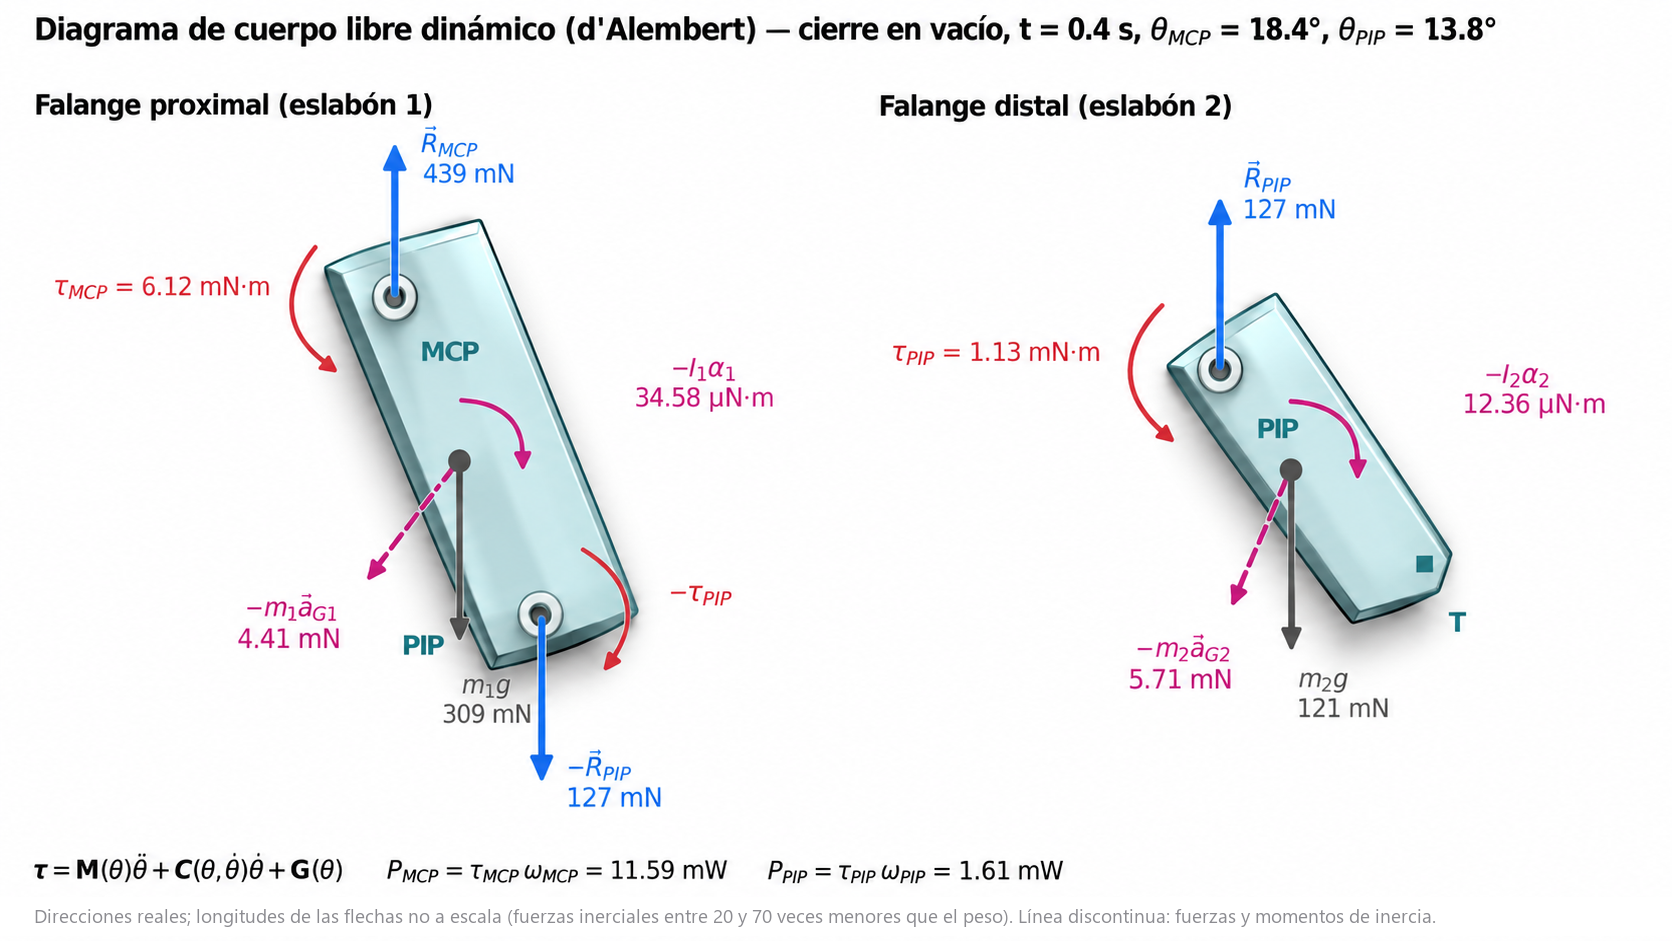
\includegraphics[width=\textwidth]{D10_DCL_dinamico_chatgpt.png}
\caption{Diagrama de cuerpo libre dinámico de las falanges en $t = 0.4$ s del cierre en vacío. Diagrama generado con el modelo y mejorado gráficamente con IA; los valores se verificaron contra el cálculo.}
\label{fig:dcldin}
\end{figure}
\par\noindent\textbf{Análisis.} Las fuerzas de inercia (4.41 y 5.71 mN) son entre 20 y 70 veces menores que los pesos de las falanges (309 y 121 mN), así que las reacciones $R_{MCP}$ = 439 mN y $R_{PIP}$ = 127 mN equivalen prácticamente al peso de lo que cuelga de cada articulación. Los torques motores (6.12 mN$\cdot$m en el MCP y 1.13 mN$\cdot$m en el PIP) equilibran sobre todo la gravedad, y la potencia instantánea es P = $\tau\omega$ = 11.59 mW en el MCP y 1.61 mW en el PIP.


\subsection{Resultados}
\begin{figure}[H]
\centering
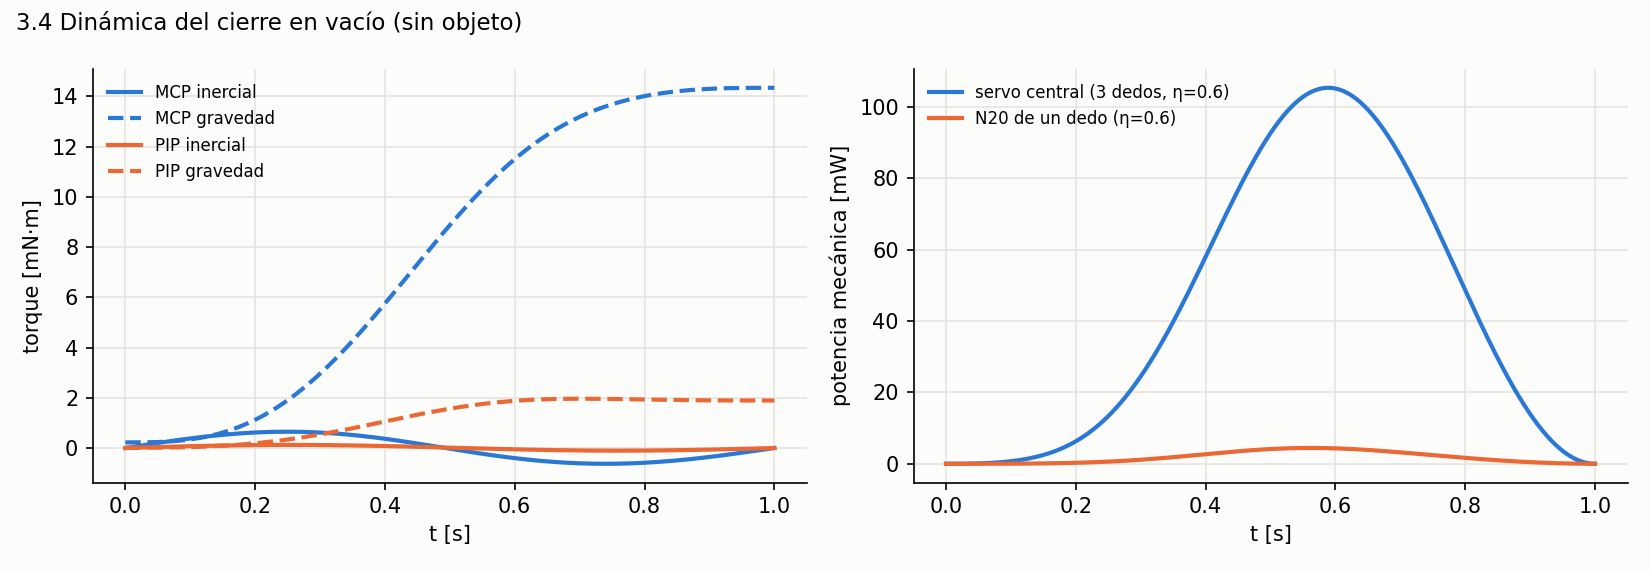
\includegraphics[width=\textwidth]{D4_dinamica_potencia.png}
\caption{Torques inerciales y gravitacionales y potencia de los motores durante el cierre.}
\label{fig:din}
\end{figure}
\par\noindent\textbf{Análisis.} Los torques inerciales no pasan de 0.65 mN$\cdot$m en el MCP y 0.12 mN$\cdot$m en el PIP, mientras que el torque total con la gravedad del dedo llega a 14.3 y 1.9 mN$\cdot$m. La potencia del servo tiene forma de campana con máximo de 105 mW cerca de t = 0.6 s, y la del N20 apenas llega a 4.4 mW: mover el dedo en vacío es barato frente a sostener una carga.




\begin{table}[H]
\centering

\begin{adjustbox}{max width=\textwidth}
\begin{tabular}{|l|r|c|}
\hline
\textbf{Magnitud} & \textbf{Valor} & \textbf{Unidad} \\ \hline
$\tau_{MCP}$ inercial máx. & 0.649 & mN$\cdot$m \\ \hline
$\tau_{PIP}$ inercial máx. & 0.124 & mN$\cdot$m \\ \hline
$\tau_{MCP}$ total máx. (inercia + gravedad) & 14.337 & mN$\cdot$m \\ \hline
$\tau_{PIP}$ total máx. & 1.891 & mN$\cdot$m \\ \hline
Potencia MCP por dedo máx. & 21.06 & mW \\ \hline
Potencia PIP por dedo máx. & 2.66 & mW \\ \hline
Potencia en el eje del servo (3 dedos, $\eta=0.6$) & 105.29 & mW \\ \hline
Potencia en el eje del N20 ($\eta=0.6$) & 4.43 & mW \\ \hline
Trabajo MCP por ciclo & 8.716 & mJ \\ \hline
Trabajo PIP por ciclo & 1.073 & mJ \\ \hline
$\Delta E_c + \Delta E_p$ & 9.789 & mJ \\ \hline
Error del balance energético & 1.2e-14 & J \\ \hline
\end{tabular}
\end{adjustbox}
\caption{Dinámica del cierre en vacío de un dedo ($t_c = 1$ s).}
\label{tab:dinamica}
\end{table}

\subsection{Energía por ciclo completo}
En la apertura la gravedad ayuda y el trabajo articular es negativo. Como el sinfín central es autobloqueante, el servo debe vencer su fricción aun así; la energía se estima con $E = |W|\tan(\phi-\lambda)/\tan\lambda$, con $\lambda = 3.6°$ y $\mu_d = 0.10$ de referencia. El sinfín PIP es reversible y la apertura del PIP no consume energía del N20.

\begin{table}[H]
\centering

\begin{adjustbox}{max width=\textwidth}
\begin{tabular}{|l|l|r|r|l|}
\hline
\textbf{Fase} & \textbf{Motor} & \textbf{Energía [mJ]} & \textbf{Potencia máx. [mW]} & \textbf{Observación} \\ \hline
Cierre & Servo (3 dedos) & 43.579 & 105.29 & Eleva los dedos ($\eta = 0.6$) \\ \hline
Cierre & N20 (por dedo) & 1.788 & 4.43 & $\eta = 0.6$ \\ \hline
Retención & Servo & 0 & 0 & Sinfín autobloqueante \\ \hline
Retención & N20 (por dedo) & $I^2 R\,t_h$ & $I^2R$ & $T = 0.444$ N$\cdot$m, eléctrica en Tabla \ref{tab:consumo} \\ \hline
Apertura & Servo (3 dedos) & 15.591 & 37.67 & Vence el autobloqueo: $|W|\,\tan(\phi-\lambda)/\tan\lambda$, factor 0.596 \\ \hline
Apertura & N20 (por dedo) & 0 & 0 & Sinfín reversible: la gravedad abre \\ \hline
\textbf{Ciclo} & \textbf{Servo} & \textbf{59.170} &  & Mecánica en el eje \\ \hline
\textbf{Ciclo} & \textbf{3 N20} & \textbf{5.365} &  & Más la retención eléctrica \\ \hline
\end{tabular}
\end{adjustbox}
\caption{Potencia y energía mecánica en los ejes de los motores en un ciclo cierre -- retención -- apertura en vacío ($t_c = 1$ s).}
\label{tab:ciclo}
\end{table}

\subsection{Consumo durante la retención}
Una vez cerrado, el sinfín central autobloqueante sostiene los MCP sin consumo. El PIP, en cambio, necesita par continuo: en un pinch de 4 kg en la punta ($\theta = 30°/30°$) el N20 de cada dedo debe entregar $T = 1.066/(4 \times 0.6) = 0.444$ N$\cdot$m de forma permanente. La potencia eléctrica de retención es $P = I^2 R$ con $I = T/K_t$, que depende de la constante de par $K_t$ y la resistencia $R$ del motor. Como el plano no especifica los motores, en la sección siguiente se estima con datos típicos de catálogo.

\subsection{Consumo eléctrico con motores típicos}
El plano no define el modelo de los motores, por lo que se usan valores típicos de catálogo (Tabla \ref{tab:motores}). Para el motor central se toma un servo digital de 20 kg$\cdot$cm (clase DS3218) en versión de rotación continua, ya que el sinfín central debe girar varias vueltas; para cada dedo, un micromotorreductor N20 de 6 V con reductora 298:1. Estos valores son supuestos y deben reemplazarse por los de la hoja de datos del motor elegido.

\begin{table}[H]
\centering

\begin{adjustbox}{max width=\textwidth}
\begin{tabular}{|l|r|r|c|}
\hline
\textbf{Parámetro} & \textbf{Servo central} & \textbf{N20 (cada dedo)} & \textbf{Unidad} \\ \hline
Tensión nominal $V$ & 6.80 & 6.00 & V \\ \hline
Velocidad en vacío $\omega_0$ & 111.0 & 100.0 & rpm \\ \hline
Par de bloqueo $T_{st}$ & 1.960 & 0.390 & N$\cdot$m \\ \hline
Corriente de bloqueo $I_{st}$ & 2.50 & 1.60 & A \\ \hline
Corriente en vacío $I_0$ & 0.15 & 0.10 & A \\ \hline
Corriente en reposo (electrónica) & 0.005 & 0.000 & A \\ \hline
Resistencia $R = V/I_{st}$ & 2.72 & 3.75 & $\Omega$ \\ \hline
Constante de par $K_t$ (eje de salida) & 0.834 & 0.260 & N$\cdot$m/A \\ \hline
Constante de f.c.e.m. $K_e$ (eje de salida) & 0.550 & 0.537 & V$\cdot$s/rad \\ \hline
Par continuo recomendado (30 \% $T_{st}$) & 0.588 & 0.117 & N$\cdot$m \\ \hline
\end{tabular}
\end{adjustbox}
\caption{Datos típicos de catálogo usados para el consumo eléctrico (supuestos, no están en el plano).}
\label{tab:motores}
\end{table}

Cada motor se representa con el modelo lineal de motor DC referido a su eje de salida:
\eq{I = I_0 + \frac{T}{K_t} \qquad V_m = I R + K_e\,\omega \qquad P_{el} = V_m\, I \qquad R = \frac{V}{I_{st}} \qquad K_t = \frac{T_{st}}{I_{st}-I_0}}
donde $T$ es el par en el eje del motor obtenido en las secciones anteriores ($T_c = \sum\tau_{MCP}/(12\eta)$, $T_i = \tau_{PIP}/(4\eta)$) y $\omega$ su velocidad. Con el motor detenido (apriete y retención) la potencia es $I^2R$; se conserva $I_0$, lo que es conservador. Se supone un driver PWM ideal que entrega solo la tensión $V_m$ necesaria.

El ciclo evaluado es: cierre hasta $\theta_{MCP} = \theta_{PIP} = 30°$ en 1.5 s (perfil cicloidal), apriete de 0.3 s hasta el par de agarre, retención de 5 s y apertura en 1.5 s. Con el cierre en 1.5 s el sinfín central necesita 80 rpm y el sinfín del N20 26.7 rpm, por debajo de las velocidades disponibles (110.8 y 99.8 rpm), así que ambos motores alcanzan el perfil. Durante la retención el sinfín central se autobloquea y el servo solo consume la corriente de reposo de su electrónica; el N20, en cambio, debe sostener el par del PIP de forma continua.

\begin{figure}[H]
\centering
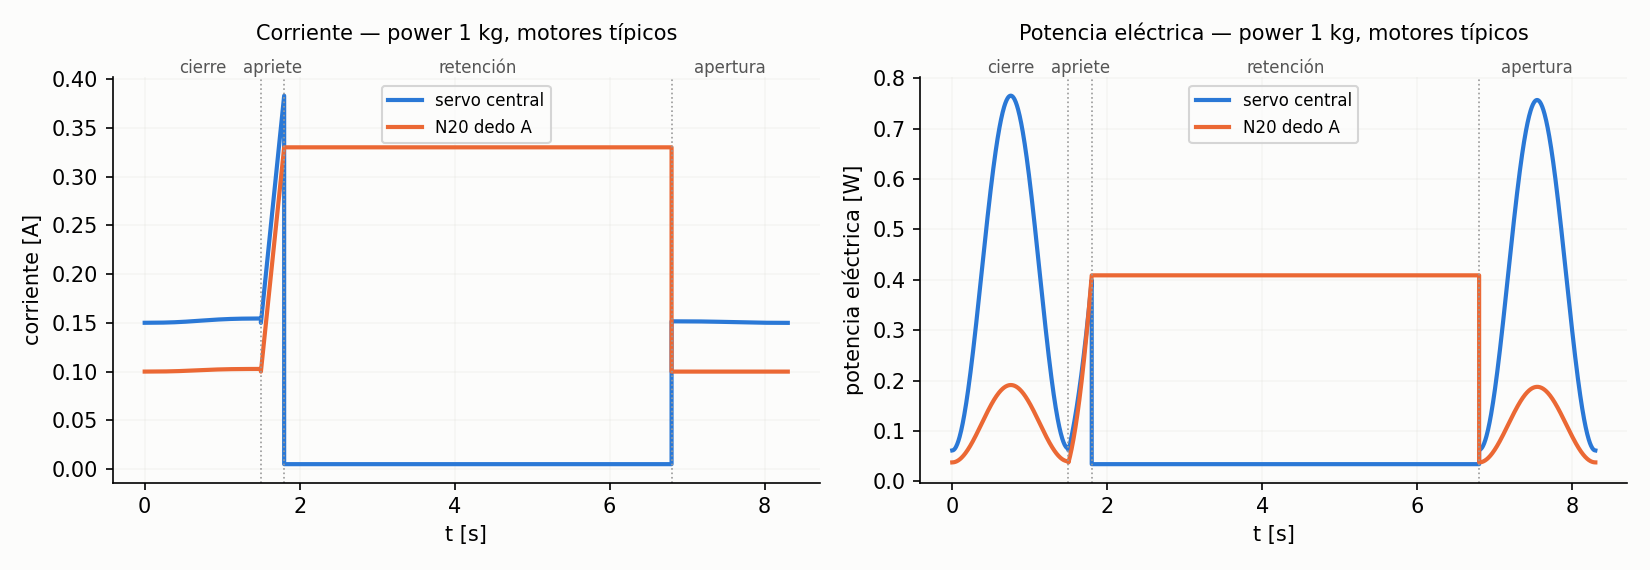
\includegraphics[width=\textwidth]{D8_consumo_electrico.png}
\caption{Corriente y potencia eléctrica del servo central y del N20 del dedo A durante un ciclo (power 1 kg).}
\label{fig:consumo}
\end{figure}
\par\noindent\textbf{Análisis.} Durante el movimiento el servo consume unos 0.15 A y el N20 0.10 A, casi solo su corriente en vacío. En el apriete la corriente sube a 0.38 A en el servo y 0.33 A en el N20. En la retención el servo baja a 5 mA porque el sinfín se autobloquea, mientras que el N20 mantiene 0.33 A durante los 5 s: esa fase representa 2.04 J de los 2.44 J que gasta el N20 en el ciclo.




La Tabla \ref{tab:resumenconsumo} resume el resultado principal: la energía por ciclo, la potencia media y si el N20 típico puede sostener el agarre.

\begin{table}[H]
\centering
\renewcommand{\arraystretch}{1.5}
\begin{tabular}{|l|r|r|>{\raggedright\arraybackslash}p{6.8cm}|}
\hline
\rowcolor{head}\textbf{Caso} & \textbf{Energía por ciclo} & \textbf{Potencia media} & \textbf{N20 típico (298:1)} \\ \hline
Power 1 kg & 6.4 J & 0.77 W & \textcolor{ok}{\checkmark\ Continuo} \\ \hline
Power 4 kg & 34.4 J & 4.14 W & \textcolor{warn}{$\triangle$\ Solo picos cortos} \\ \hline
Pinch 1 kg & 13.5 J & 1.62 W & \textcolor{ok}{\checkmark\ Continuo} \\ \hline
Pinch 4 kg & 128 J & 15.45 W & \textcolor{bad}{$\times$\ No viable: necesita 0.444 N$\cdot$m, por encima de su par de bloqueo de 0.39 N$\cdot$m} \\ \hline
\end{tabular}
\caption{\textbf{Resumen de consumo eléctrico y viabilidad del motor de dedo.} Ciclo de 8.3 s (cierre, apriete, retención de 5 s y apertura), motores típicos de catálogo.}
\label{tab:resumenconsumo}
\end{table}

\begin{table}[H]
\centering

\begin{adjustbox}{max width=\textwidth}
\begin{tabular}{|l|r|r|r|r|r|r|r|}
\hline
\textbf{Fase} & \textbf{Duración [s]} & \textbf{$I_{servo}$ máx. [A]} & \textbf{$P_{servo}$ máx. [W]} & \textbf{$E_{servo}$ [J]} & \textbf{$I_{N20}$ máx. [A]} & \textbf{$P_{N20}$ máx. [W]} & \textbf{$E_{N20}$ [J]} \\ \hline
Cierre & 1.50 & 0.155 & 0.766 & 0.621 & 0.103 & 0.191 & 0.172 \\ \hline
Apriete & 0.30 & 0.383 & 0.399 & 0.062 & 0.330 & 0.409 & 0.057 \\ \hline
Retención & 5.00 & 0.005 & 0.034 & 0.170 & 0.330 & 0.409 & 2.044 \\ \hline
Apertura & 1.50 & 0.152 & 0.757 & 0.614 & 0.100 & 0.188 & 0.169 \\ \hline
\end{tabular}
\end{adjustbox}
\caption{Consumo por fase en el caso power 1 kg (N20 del dedo más cargado).}
\label{tab:fases}
\end{table}
\begin{table}[H]
\centering

\begin{adjustbox}{max width=\textwidth}
\begin{tabular}{|l|r|r|c|r|r|r|c|r|r|r|r|}
\hline
\textbf{Caso} & \textbf{$T_c$ [N$\cdot$m]} & \textbf{$I_{servo}$ [A]} & \textbf{Servo} & \textbf{$T_{N20}$ [N$\cdot$m]} & \textbf{$I_{N20}$ [A]} & \textbf{$P_{ret}$ [W]} & \textbf{N20} & \textbf{$E_{servo}$ [J]} & \textbf{$E_{3\,N20}$ [J]} & \textbf{$E_{ciclo}$ [J]} & \textbf{$\bar P$ [W]} \\ \hline
Power 1 kg (D) & 0.195 & 0.38 & Continuo & 0.060 & 0.33 & 0.41 & Continuo & 1.47 & 4.94 & 6.41 & 0.77 \\ \hline
Power 4 kg (D) & 0.767 & 1.07 & Solo pico & 0.237 & 1.01 & 3.85 & Solo pico & 1.77 & 32.62 & 34.39 & 4.14 \\ \hline
Pinch 1 kg (T) & 0.229 & 0.42 & Continuo & 0.112 & 0.53 & 1.05 & Continuo & 1.48 & 11.98 & 13.46 & 1.62 \\ \hline
Pinch 4 kg (T) & 0.905 & 1.23 & Solo pico & 0.444 & 1.81 & 12.25 & \textbf{Excede} & 1.88 & 126.36 & 128.23 & 15.45 \\ \hline
\end{tabular}
\end{adjustbox}
\caption{Consumo eléctrico por ciclo con motores típicos: cierre 1.5 s, apriete 0.3 s, retención 5 s y apertura 1.5 s, agarre a 30°/30°, $\mu = 0.5$, $\eta = 0.6$. $I_{N20}$ y $P_{ret}$ corresponden al dedo más cargado.}
\label{tab:consumo}
\end{table}

En la Tabla \ref{tab:consumo}, ``Continuo'' indica que el par no supera el 30 \% del par de bloqueo, ``Solo pico'' que lo supera pero queda por debajo del bloqueo, y ``Excede'' que el motor típico no puede entregarlo. Para el servo, ``Solo pico'' es aceptable porque el par de agarre solo se mantiene durante el apriete (0.3 s) y luego el sinfín autobloqueante lo sostiene.

\subsection{Análisis de resultados dinámicos}
\begin{itemize}
\item Los torques inerciales son menores a 1 mN$\cdot$m y no condicionan la selección de los motores; el dimensionamiento lo fija la carga estática del agarre.
\item Un ciclo completo en vacío requiere 59.2 mJ en el eje del servo y 5.4 mJ entre los tres N20.
\item El cierre en vacío requiere 9.8 mJ por dedo y una potencia máxima de 105 mW en el eje del servo con $\eta = 0.6$.
\item El balance energético cierra con error de $10^{-14}$ J, lo que valida la formulación dinámica.
\item Con motores típicos, un ciclo de 8.3 s con 1 kg en power consume 6.4 J (0.77 W en promedio); con 4 kg sube a 34.4 J (4.1 W). El servo aporta menos de 1.9 J por ciclo en todos los casos porque el sinfín autobloqueante le permite apagarse durante la retención.
\item Entre el 77 \% y el 99 \% de la energía del ciclo la consumen los N20 al retener el PIP. En un pinch de 4 kg en la punta el N20 típico tendría que dar 0.444 N$\cdot$m, por encima de su par de bloqueo (0.39 N$\cdot$m), así que ese caso no es viable con un N20 298:1.
\item El mayor consumo energético del sistema proviene de la retención en el PIP, por lo que se recomienda un tren autobloqueante o un freno en esa articulación: eliminaría casi todo el consumo de retención.
\end{itemize}

% ======================================================================
\section{Simulación en Working Model 2D}
\subsection{Modelo estático}
Se construyó un modelo de Working Model 2D en vista lateral con los tres dedos y la palma. Cada articulación fija su ángulo con un actuador de posición, que mide el torque necesario en esa articulación, y las fuerzas de contacto se aplican en P, D o T. Un barrido automático recorrió 180 configuraciones.

\begin{figure}[H]
\centering
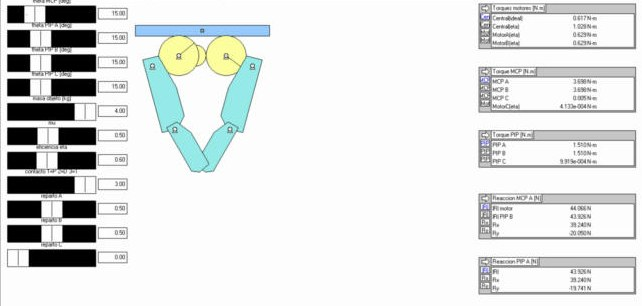
\includegraphics[width=0.8\textwidth]{wm_estatica.jpg}
\caption{Modelo estático en Working Model 2D.}
\label{fig:wmest}
\end{figure}
\par\noindent\textbf{Análisis.} El modelo reproduce el dedo con sus articulaciones motorizadas, los contactos P, D y T y los medidores de torque y reacción en el MCP y el PIP. En el barrido de 180 configuraciones la diferencia máxima con el cálculo analítico fue 0.034 \%, lo que confirma la geometría del plano y la convención de signos.




\begin{table}[H]
\centering

\begin{adjustbox}{max width=\textwidth}
\begin{tabular}{|l|r|r|c|}
\hline
\textbf{Magnitud} & \textbf{Error máx. [\%]} & \textbf{Error medio [\%]} & \textbf{Casos $>5$ \%} \\ \hline
Torque motor central & 0.0009 & 0.0002 & 0 \\ \hline
Torque motor A & 0.0279 & 0.0067 & 0 \\ \hline
Torque motor B & 0.0279 & 0.0067 & 0 \\ \hline
Torque motor C & 0.0279 & 0.0112 & 0 \\ \hline
$\tau_{MCP}$ dedo A & 0.0009 & 0.0002 & 0 \\ \hline
$\tau_{MCP}$ dedo B & 0.0009 & 0.0002 & 0 \\ \hline
$\tau_{MCP}$ dedo C & 0.0341 & 0.0110 & 0 \\ \hline
$\tau_{PIP}$ dedo A & 0.0341 & 0.0104 & 0 \\ \hline
$\tau_{PIP}$ dedo B & 0.0341 & 0.0104 & 0 \\ \hline
$\tau_{PIP}$ dedo C & 0.0341 & 0.0172 & 0 \\ \hline
Reacción MCP dedo A & 0.0002 & 0.0002 & 0 \\ \hline
Reacción PIP dedo A & 0.0341 & 0.0114 & 0 \\ \hline
Reacción PIP dedo B & 0.0341 & 0.0114 & 0 \\ \hline
Fuerza normal dedo A & 0.0000 & 0.0000 & 0 \\ \hline
Fuerza tangencial dedo A & 0.0000 & 0.0000 & 0 \\ \hline
\end{tabular}
\end{adjustbox}
\caption{Comparación analítico vs Working Model 2D en 180 configuraciones.}
\label{tab:wm}
\end{table}

\subsection{Pruebas de agarre en el modelo estático}
El modelo estático se evaluó en cuatro pruebas con un objeto de 4 kg, $\mu = 0.5$ y $\theta_{MCP} = \theta_{PIP} = 15^\circ$. Las figuras muestran la ventana de Working Model en cada prueba, con los controles a la izquierda y los medidores a la derecha. La Tabla~\ref{tab:pruebaswm} resume los valores leídos.

\begin{table}[H]
\centering
\caption{Resultados de las pruebas en Working Model 2D (dedos A / B / C).}
\label{tab:pruebaswm}
\begin{adjustbox}{max width=\textwidth}
\begin{tabular}{|l|c|c|c|}
\hline
\textbf{Prueba} & \textbf{$N$ [N]} & \textbf{$\tau_{MCP}$ [N$\cdot$m]} & \textbf{$\tau_{PIP}$ [N$\cdot$m]} \\ \hline
Pinch (T) & 39.24 / 39.24 / 0 & 3.698 / 3.698 / 0.005 & 1.510 / 1.510 / 0.001 \\ \hline
Power 120° (D) & 26.16 / 26.16 / 26.16 & 2.072 / 2.072 / 2.072 & 0.611 / 0.611 / 0.611 \\ \hline
Power plano (D) & 39.24 / 19.62 / 19.62 & 3.105 / 1.555 / 1.555 & 0.917 / 0.459 / 0.459 \\ \hline
Desigual (T) & 31.39 / 27.47 / 19.62 & 2.960 / 2.590 / 1.852 & 1.208 / 1.057 / 0.756 \\ \hline
\end{tabular}
\end{adjustbox}
\end{table}

\begin{figure}[H]
\centering
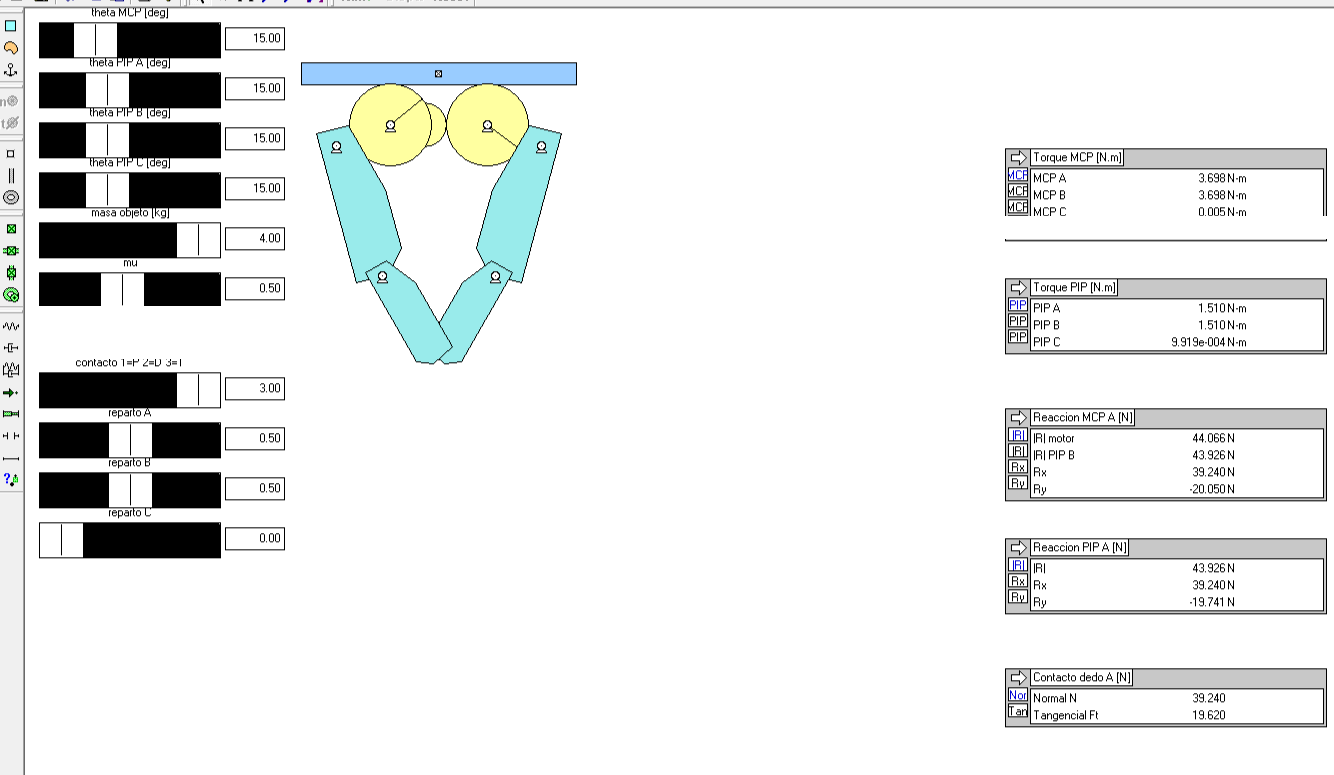
\includegraphics[width=0.9\textwidth]{wm_prueba_pinch_sin_motores.png}
\caption{Prueba Pinch en Working Model 2D (contacto en T, reparto 50/50/0).}
\label{fig:wmpinch}
\end{figure}
\par\noindent\textbf{Análisis.} Los dedos A y B se reparten la carga por igual (39.24 N y 3.698 N$\cdot$m en cada MCP) y C queda prácticamente sin carga (0.005 N$\cdot$m, solo por su peso). Es la prueba más exigente para las articulaciones: 3.698 N$\cdot$m en el MCP y 1.510 N$\cdot$m en el PIP de A y B.




\begin{figure}[H]
\centering
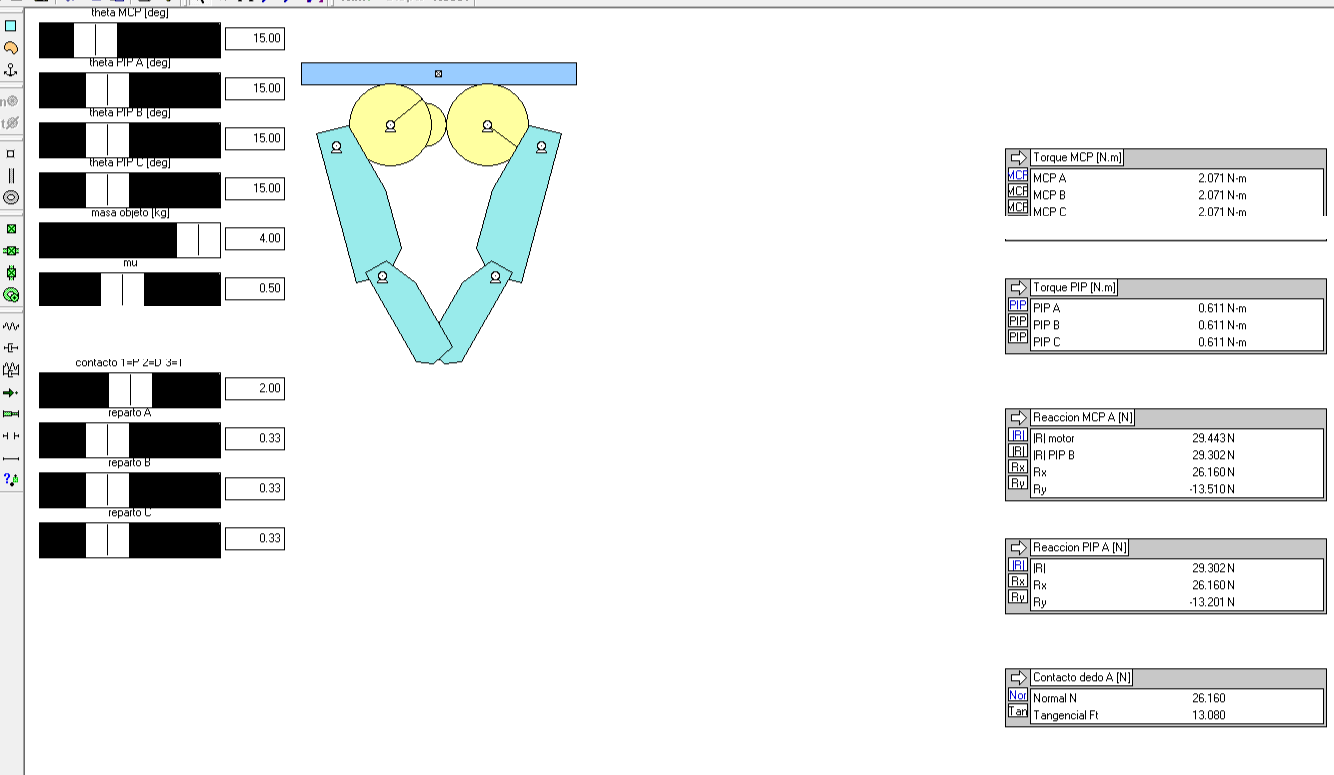
\includegraphics[width=0.9\textwidth]{wm_prueba_power120_sin_motores.png}
\caption{Prueba Power 120° en Working Model 2D (contacto en D, reparto igual).}
\label{fig:wmpower120}
\end{figure}
\par\noindent\textbf{Análisis.} Con los dedos a 120° la carga se reparte por igual: 26.16 N y 2.072 N$\cdot$m en cada MCP. Es la prueba más favorable: el PIP más cargado necesita solo 0.611 N$\cdot$m, el menor máximo de las cuatro pruebas.




\begin{figure}[H]
\centering
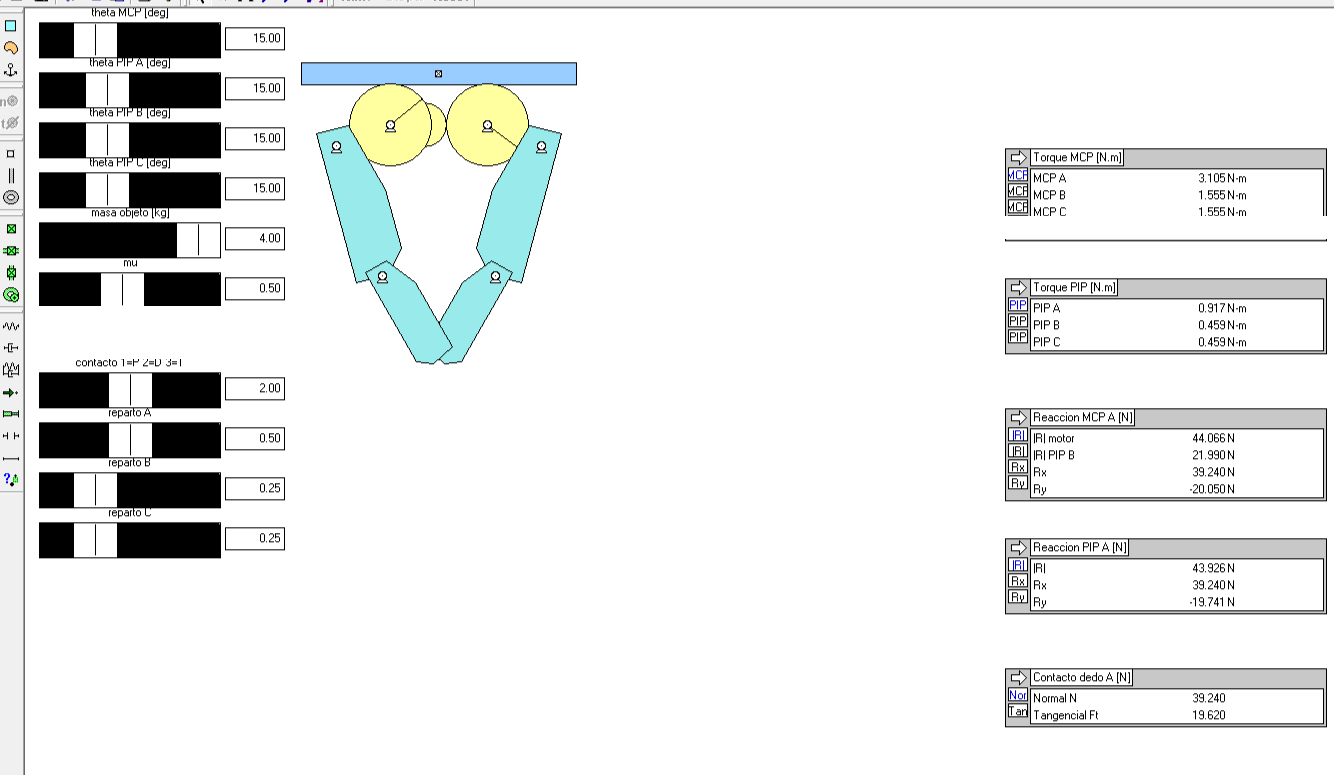
\includegraphics[width=0.9\textwidth]{wm_prueba_plano_sin_motores.png}
\caption{Prueba Power plano V2.4 en Working Model 2D (contacto en D, reparto 50/25/25).}
\label{fig:wmplano}
\end{figure}
\par\noindent\textbf{Análisis.} Con la disposición real, A se opone a B y C y debe hacer el doble de fuerza (39.24 N frente a 19.62 N). La suma de torques MCP es la misma que en el power a 120° (6.214 N$\cdot$m), pero se concentra en A: 3.105 N$\cdot$m en su MCP y 0.917 N$\cdot$m en su PIP.




\begin{figure}[H]
\centering
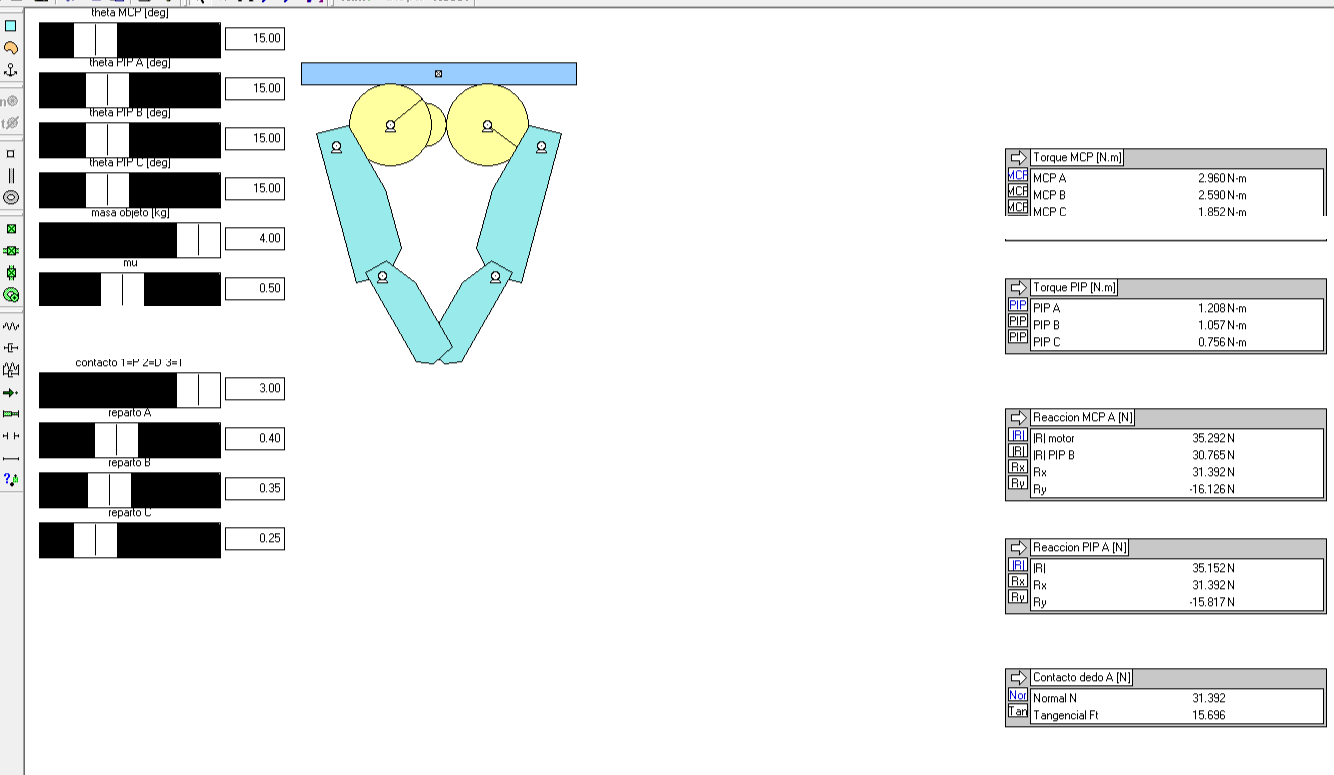
\includegraphics[width=0.9\textwidth]{wm_prueba_desigual_sin_motores.png}
\caption{Prueba Carga desigual en Working Model 2D (contacto en T, reparto 40/35/25).}
\label{fig:wmdesigual}
\end{figure}
\par\noindent\textbf{Análisis.} Con el reparto 40/35/25 los torques siguen exactamente la proporción de la carga (2.960, 2.590 y 1.852 N$\cdot$m en los MCP). La suma de torques MCP (7.402 N$\cdot$m) es la misma del pinch, porque la carga total y el punto de contacto son los mismos.




\subsection{Modelo dinámico}
El modelo dinámico se acciona por torque. El tren central se representa con engranes 1/30 y 2.5, cada dedo tiene un piñón z12 unido a la falange por la rigidez torsional del engrane y el objeto es un cilindro de 46 mm con fricción. Con 1 kg y $\mu = 0.5$ el objeto cae para $T_c \leq 0.20$ N$\cdot$m y queda sostenido para $T_c \geq 0.25$ N$\cdot$m. Con $T_c = 1.0$ N$\cdot$m el torque en cada MCP converge a 3.589 N$\cdot$m, frente a 3.6 N$\cdot$m teóricos.

\begin{figure}[H]
\centering
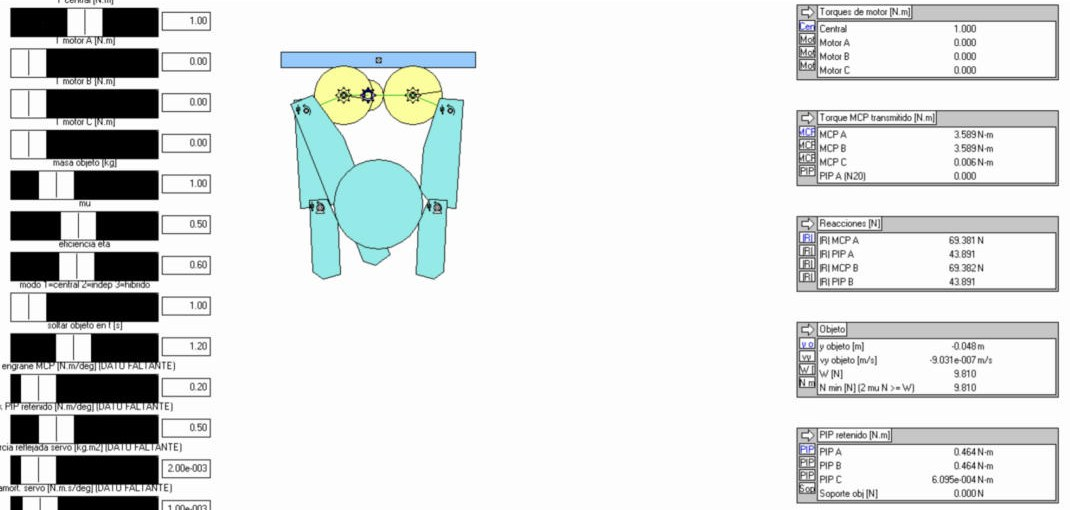
\includegraphics[width=0.85\textwidth]{wm_agarre.jpg}
\caption{Modelo dinámico sosteniendo un objeto de 1 kg.}
\label{fig:wmdin}
\end{figure}
\par\noindent\textbf{Análisis.} Con 1 kg y $\mu$ = 0.5 el objeto se sostiene a partir de $T_c$ = 0.25 N$\cdot$m y cae con 0.20 N$\cdot$m, lo que acota el par mínimo del servo para esa carga. Con $T_c$ = 1.0 N$\cdot$m el torque en cada MCP converge a 3.589 N$\cdot$m frente a 3.6 N$\cdot$m teóricos, una diferencia de 0.3 \%.




% ======================================================================
\section{Conclusiones}
\begin{itemize}
\item El análisis estático en las tres vistas permitió determinar las fuerzas de contacto, los torques articulares, y las reacciones para todas las combinaciones de postura, contacto, masa y fricción, sin considerar la transmisión de engranajes. El caso crítico corresponde al pinch de punta con dedos rectos y fricción baja.
\item La disposición del plano V2.4, con el dedo A opuesto a los dedos B y C, hace que el dedo A soporte el doble de fuerza normal que cada uno de los otros dos en un agarre de potencia.
\item El análisis cinemático entregó las posiciones, velocidades y aceleraciones lineales y angulares de las falanges, y las velocidades requeridas en los motores para un tiempo de cierre dado.
\item El análisis dinámico mostró que los efectos inerciales son despreciables frente a las cargas de agarre y que el mayor consumo de energía se produce en la retención del PIP.
\item Con el caso de diseño 2 (3.5 kg y $\mu = 0.3$) la normal sube un 46 \% y los torques en las articulaciones alrededor de un 35 \% respecto a 4 kg con $\mu = 0.5$: el caso crítico pide 5.104 N$\cdot$m en el MCP y 2.157 N$\cdot$m en el PIP, y la raíz de la falange proximal soporta 4.91 N$\cdot$m de flexión.
\item La simulación en Working Model 2D validó el cálculo analítico con un error máximo de 0.034 \% en 180 configuraciones y reprodujo el comportamiento de agarre de los tres modos de accionamiento.
\item Con motores típicos, el consumo eléctrico por ciclo va de 6.4 J (power 1 kg) a 128 J (pinch 4 kg), y la retención del PIP con los N20 es la que lo determina. El N20 típico 298:1 sostiene de forma continua los agarres de 1 kg, solo admite picos cortos en el power de 4 kg y no puede sostener el pinch de 4 kg en la punta (Tabla \ref{tab:resumenconsumo2}).
\end{itemize}

\begin{table}[H]
\centering
\renewcommand{\arraystretch}{1.5}
\begin{tabular}{|l|r|r|>{\raggedright\arraybackslash}p{6.8cm}|}
\hline
\rowcolor{head}\textbf{Caso} & \textbf{Energía por ciclo} & \textbf{Potencia media} & \textbf{N20 típico (298:1)} \\ \hline
Power 1 kg & 6.4 J & 0.77 W & \textcolor{ok}{\checkmark\ Continuo} \\ \hline
Power 4 kg & 34.4 J & 4.14 W & \textcolor{warn}{$\triangle$\ Solo picos cortos} \\ \hline
Pinch 1 kg & 13.5 J & 1.62 W & \textcolor{ok}{\checkmark\ Continuo} \\ \hline
Pinch 4 kg & 128 J & 15.45 W & \textcolor{bad}{$\times$\ No viable: necesita 0.444 N$\cdot$m, por encima de su par de bloqueo de 0.39 N$\cdot$m} \\ \hline
\end{tabular}
\caption{\textbf{Resumen de consumo eléctrico y viabilidad del motor de dedo.} Ciclo de 8.3 s (cierre, apriete, retención de 5 s y apertura), motores típicos de catálogo.}
\label{tab:resumenconsumo2}
\end{table}

% ======================================================================
\appendix
\section{Datos faltantes del plano}
Los siguientes parámetros no están en el plano V2.4 y se trataron como variables: curva par--velocidad y par máximo del servo y del N20, reducción interna del N20, fricción entre dientes de los sinfines, ángulo de presión de los engranes, mano de los sinfines B y C, eficiencia del par z20, espesor y masa de la palma, diámetro del objeto, rigidez torsional de los trenes e inercia y amortiguamiento equivalentes de los motores.

\end{document}
